\fancyhead[L]{\hyperref[chapter:quantification]{\textsc{Quantification}}}
\chapter{Quantification}\label{chapter:quantification}
\localtableofcontents
\addcontentsline{lot}{chapter}{Quantification}
\addcontentsline{lof}{chapter}{Quantification}
\addcontentsline{tof}{chapter}{Quantification}
\fancyhead[L]{\hyperref[chapter:quantification]{\textsc{Quantification}}}

\clearpage

\breaksection{Introduction}

In the FutuRaM project, scenario elements are categorised based on their influence and relevance to the secondary raw material (SRM) system. This categorisation aids in refining the focus of the scenarios and ensuring they are relevant, manageable, and useful.

Following the process detailed in \autoref{chapter:methodology}, the resultant scenario elements were classified in preparation for quantification. These elements are listed in \autoref{tab:elements-4}.

\begin{description}[style=nextline]
    \item[Internal Elements:](\autoref{sec:quantification_internal_rec} and \autoref{sec:quantification_internal_cei})
    These are directly within the scope of FutuRaM and significantly impact the waste management system. They are integral to the models and scenarios. For example, changes in waste composition and recovery methods fall under this category. These elements are thoroughly researched and modeled as they are central to understanding and projecting the SRM system's future.
    \item[External Elements:](\autoref{sec:quantification_external})
    Elements deemed external are still relevant to the scenarios but are not as directly related as the internal elements. External elements are set as the background of the three scenarios, allowing a better focus on the main variables of importance to FutuRaM. These elements do not vary across the three different scenarios but they do change over time. These elements include demographics, economic growth, and the renewable energy transition.
    \item[Outside Elements:](\autoref{sec:quantification_external})
    These are factors outside the scope and influence of the waste management system and are not included in the scenario storylines or directly in the models. They may be considered in sensitivity analysis but are not primary drivers in the scenario development. For instance, resource supply constraints are external factors that could impact the waste management system but are too unpredictable and complex to model directly within the scenarios. Their inclusion could introduce significant uncertainty and make the models less interpretable and actionable. These elements are, however, considered important, and their possible impacts on the SRM system will be explored in exercises of sensitivity analysis and optimisation. 
  \end{description}

The rationale behind this categorisation is to maintain focus and clarity in the scenario modeling. Including too many complex and indirectly related elements can convolute the scenarios, making them overly complex and less useful for practical decision-making and policy analysis. By concentrating on integral elements --- or those that can be controlled or influenced by associated policy decisions --- FutuRaM ensures that its scenarios are both manageable and directly relevant to its objectives of exploring different futures of the SRM system. This approach strikes a balance between realism and practicality, ensuring the scenarios are both meaningful and actionable.


\subsection{Quantification and Implementation of scenario elements in the models}

\subsubsection{External drivers}

For each external driver in the scenarios, the values are defined globally and each waste stream will interpret this into their models using a "top-down" approach. This will require the development of correlations between the scenario driver and the parameter in the waste stream model. The resolution of this will be different for each scenario driver and each waste stream. 

\subsubsection{Internal elements}

For the internal elements in the scenarios, a global value can often not be defined. For these elements, the waste stream models will define the values for each scenario using a "bottom-up" approach. This will require the estimation of future trends for each parameter and scenario for the product/waste groupings in each waste stream. Then, a global value can be calculated by taking a weighted average for each of the groups. 

The outcome of these estimations will be a range of values for each time series, for each parameter in each waste stream for each scenario.

\autoref{fig:quantification_diagram} depicts a schema for the interconnection between the models for the quantification and implementation of the scenario elements. 

\begin{landscape}
  \begin{figure}[h]
    \centering
    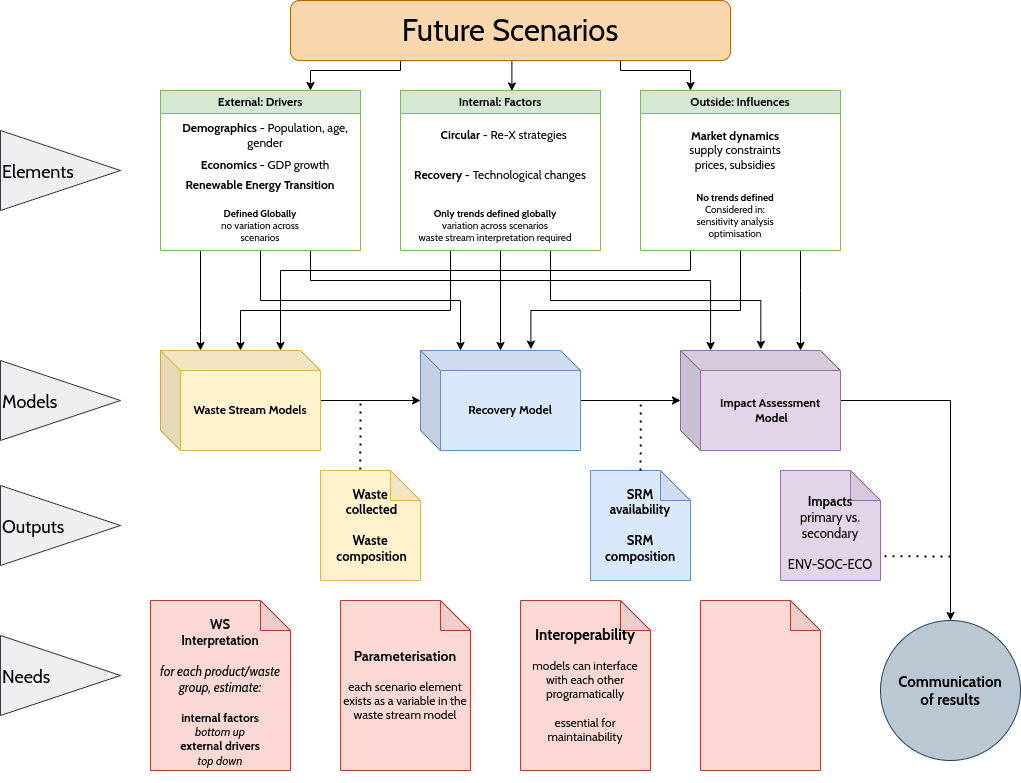
\includegraphics[width=0.8\linewidth]{130quantification/scenario_schema.drawio.png}
    \caption{Quantification and Implementation of scenario elements in the models}
    \label{fig:quantification_diagram}
    \end{figure}
\end{landscape}

\subsubsection{Methodology for quantification}

The methodology for quantification of the scenario elements is as follows:

\begin{enumerate}
  \item Define the parameters for each waste stream model
  \item Define the parameters for each scenario element in relation to the parameters in the waste stream model
  \item Define the correlations between the scenario elements and the parameters
  \item Estimate the future trends for each parameter in each scenario for every set of product/waste groupings
  \item Using the constraints of the waste stream parameter for each product group, define the coefficients of the functions between the scenario elements and the parameters
\end{enumerate}


\autoref{fig:quantification_diagram_correlations} depicts a schema for the development of correlations between elements and parameters in the waste stream models and the scenarios. The values of the functions between the pairs need to be defined.

\begin{landscape}
  \begin{figure}[h]
    \centering
    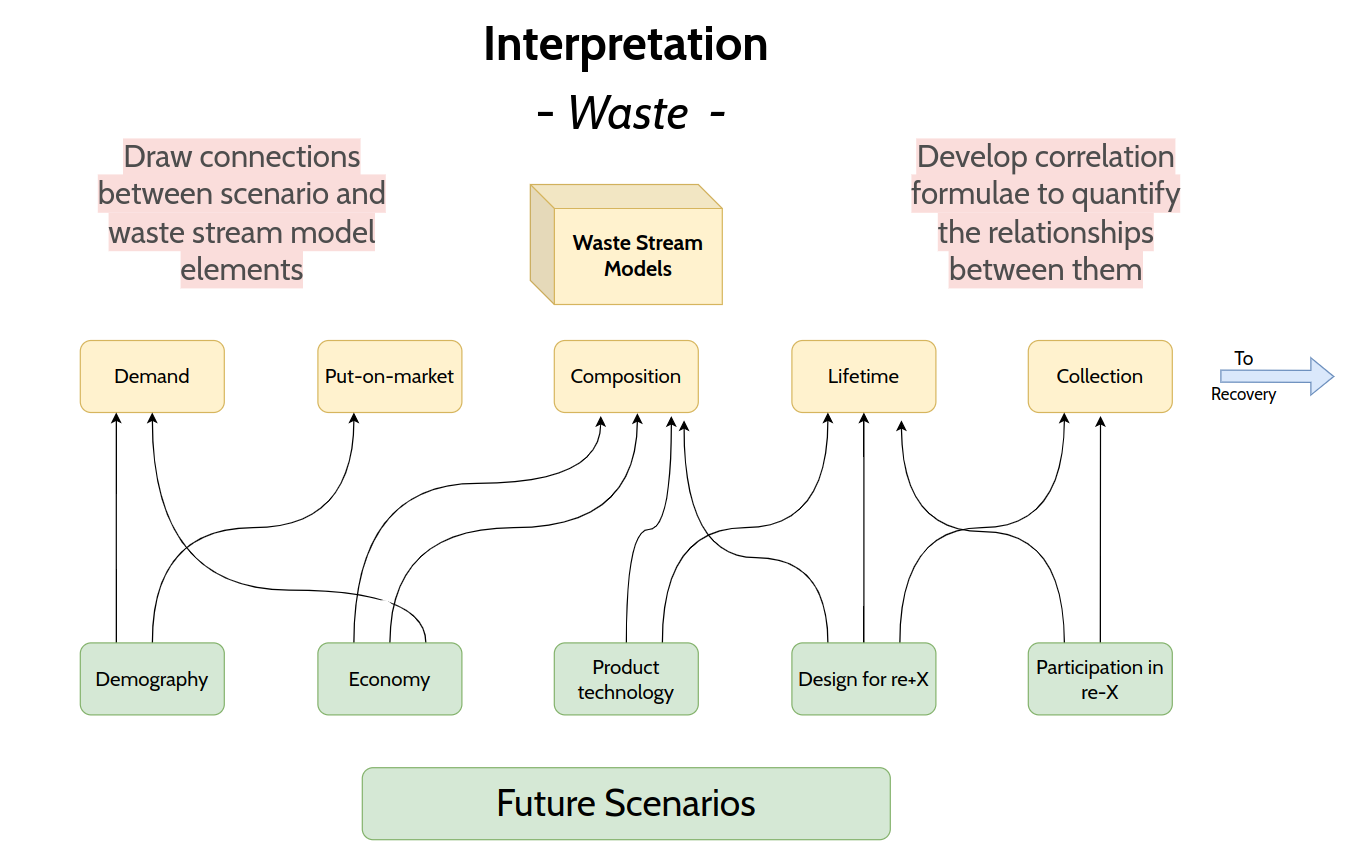
\includegraphics[width=\linewidth]{130quantification/scenario_schema_correlations.png}
    \caption{Development of correlations between elements and parameters in the waste stream models and the scenarios}
    \label{fig:quantification_diagram_correlations}
    \end{figure}
\end{landscape}

\subsubsection{Methodology for estimating future trends}

After the correlations between the scenario elements and the parameters in the waste stream models have been defined, the future trends for each parameter in each scenario for every set of product/waste groupings can be estimated.

For some parameters, the future trends can be estimated using a simple linear regression. For other parameters, the future trends will be estimated using a more complex model. The exact methodology for estimating the future trends for each parameter in each scenario for every set of product/waste groupings will be determined on a case-by-case basis.

Consideration of historical and current data, knowledge of the waste stream, and analysis of the scenarios will be used to determine the most appropriate modelling method.

An exact value is not to be sought, but rather a distribution, with constraints regarding the minimum and maximum values and the rate of change over time.

Using this, simple models can be approximated using the method of curve fitting. The choice of model (linear, exponential, etc.) will be determined by the data and the scenario. For example, a new technology or a rapid change in policy may result in an initial exponential change in the parameter, the beginning of the typical sigmoidal curve (or even a step change). This may then level off to a linear trend, then a logarithmic relationship as the technology or policy matures.

\autoref{fig:dinosaurs2013scurve} illustrates a sigmoidal curve with its characteristic three phases of growth. Typically, a sigmoidal curve (depicted as a solid black line) commences with an exponential phase, transitions into a linear phase (encompassing the inflection point where the growth rate peaks), and concludes with an asymptotic phase, where the curve nears a constant asymptote 'a' as time tends towards infinity. In certain instances, the initial exponential phase might be remarkably brief, to the point of seeming non-existent. However, the linear and asymptotic stages are consistent features across all sigmoidal curves. Attenuating curves share similarities but are distinct in that they do not have the initial exponential phase, resembling a sigmoidal curve that initiates at its inflection point around t\~0. The logistic function is a special case of the sigmoidal function, with the inflection point at x=0.

\begin{figure}[h!]
  \centering
  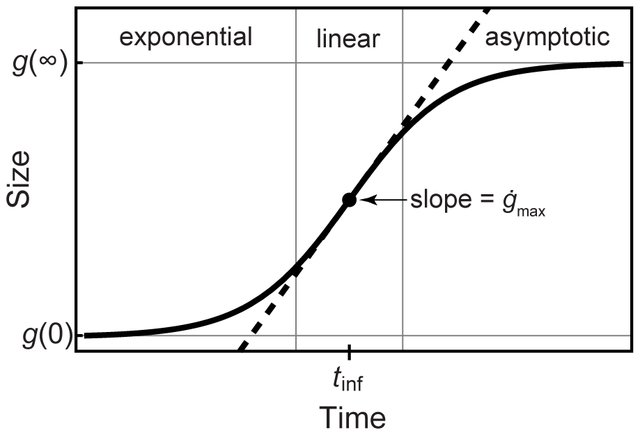
\includegraphics[width=0.8\linewidth]{130quantification/dinosaurs2013scurve.jpg}
  \caption{An example of a sigmoidal function (s-curve)}
  \label{fig:dinosaurs2013scurve}
\end{figure}

The s-curve is a generalisation of the logistic function, which is defined as:

\begin{equation}
  f(x) = \frac{L}{1+e^{-k(x-x_0)}}
\end{equation}

where:

\begin{itemize}
  \item $x_0$ = the x-value of the sigmoid's midpoint,
  \item $L$ = the curve's maximum value, and
  \item $k$ = the logistic growth rate or steepness of the curve.
  \item $e$ = the natural logarithm base (also known as Euler's number),
\end{itemize}

Important to note here is that what, during some period, may appear to be a constant linear (or other) change, may in fact be a segment of a sigmoidal curve. This is important to consider when estimating future trends, for some changes, the period from 2020-2050 may be short enough that the nature of the transition does not change, although it would when viewed over a longer time range.

\begin{samepage}
The comic in \autoref{fig:xkcd-sustainable} plots the frequency of the usage of the term 'sustainable' over time, forecasting that by 2109, all sentences will consist only of the word 'sustainable', repeated again and again. `Fittingly', the author also notes that '100 years is a lot longer than many of our resources will last'. 

\begin{figure}[ht!]
  \centering
  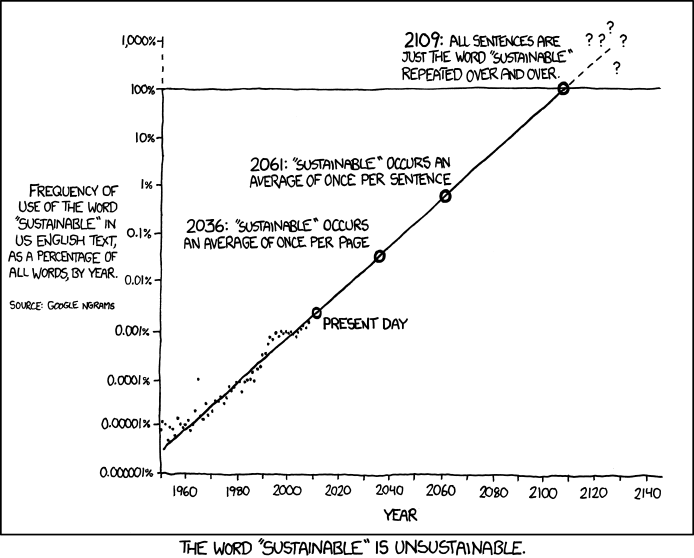
\includegraphics[width=0.8\linewidth]{130quantification/xkcd-sustainable.png}
  \caption[The word 'sustainable' is unsustainable]{The word 'sustainable' is unsustainable~\cite{xkcd-sustainable}}
  \label{fig:xkcd-sustainable}
\end{figure}
\end{samepage}

It is of course a generalisation to assume that all growth rates follow this trend, but it is mostly close enough to reality to be useful. This will be the standard approach for estimating future trends in the FutuRaM project unless there is reason to believe that the nature of the transition is different (which it often is!). 

Further details are provided in the relevant sections of this chapter and will be updated as the project progresses.

\clearpage


\breaksection{Summary}\label{sec:quantification_summary}


\boxreview{This summary will be compiled once the individual waste stream sections for each parameter are complete.}
\clearpage

\breaksection{External elements}\label{sec:quantification_external}

\subsection{Introduction}

\boxgreen{\textbf{External drivers}}{
        \textbf{Scenario elements}
        \begin{itemize}
          \item \textbf{Demographic change:} \\ population, median age, urbanisation, gender 
          \item \textbf{Economic growth:} \\ GDP
          \item \textbf{Renewable energy transition:} \\ energy mix
        \end{itemize}
        \textbf{Waste model parameters include:}
        \begin{itemize}
          \item \textbf{Put-on-market}
          \item \textbf{Composition}
        \end{itemize}
        \textbf{Recovery model parameters include:}
        \begin{itemize}
          \item \textbf{Recovery processes:} \\ market penetration of recovery technologies
          \item \textbf{Transfer coefficients:} \\ function of recovery technologies
          \item \textbf{Recovery system size:} \\ BAU - set by trends in BAU, CIR \& REC - defined by model outcomes within constraints
        \end{itemize}
        \textbf{Impact model parameters include:}
        \begin{itemize}
          \item \textbf{Foreground inventory:} \\ inputs and outputs of recovery system
          \item \textbf{Background inventory:}\\  energy mix, impact of primary production
        \end{itemize}
          }


In the FutuRaM project, scenario elements are categorised based on their influence and relevance to the secondary raw material (SRM) system. This categorization aids in refining the focus of the scenarios and ensuring they are relevant, manageable and useful.

Following the process detailed in \autoref{chapter:methodology}, several scenario elements were classified as "external" or "outside". 

The following "external" elements are incorporated into the scenarios as background information but are not directly modelled. They are assumed to be constant across the three scenarios, but change over time.

\begin{itemize}
    \item Demographic change 
    \item Economic growth  
    \item Renewable energy transition 
\end{itemize}

The following "outside" elements are not incorporated into the scenarios, but are considered important and will be explored in sensitivity analysis and optimisation.

\begin{itemize}
    \item Resource supply constraints 
    \item International trade and co-operation 
    \item Re-industrialisation of EU 
    \item Resistance to recovery projects ("NIMBY") 
\end{itemize}

These elements are detailed in \autoref{tab:elements-external}.

\begin{landscape}
\begin{table}[h!]
    \centering
    \small
    \caption{List of external scenario elements}\label{tab:elements-external}
    \begin{tabular}{|C{1.5cm}|L{6cm}|C{1.5cm}|C{1.5cm}|C{1.5cm}|C{1cm}|C{1cm}|C{1cm}|L{6cm}|}
      \hline
      \rowcolor{headerblue} % Applying the header color
      \textcolor{white}{\textbf{DOMAIN}} & \textcolor{white}{\textbf{ELEMENT}} & \textcolor{white}{\textbf{INTERNAL}} & \textcolor{white}{\textbf{EXTERNAL}} & \textcolor{white}{\textbf{OUTSIDE}} & \textcolor{white}{\textbf{BAU}} & \textcolor{white}{\textbf{REC}} & \textcolor{white}{\textbf{CIR}} & \textcolor{white}{\textbf{MODEL PARAMETERS AFFECTED}} \\
      \hline
      ECO & Progress toward renewable energy targets & & \checkmark & & - & - & - & composition, demand, waste generation, recovery impacts \\
      ECO & Economic growth & & \checkmark & & - & - & - & composition, demand, waste generation \\
      SOC & Population & & \checkmark & & - & - & - & demand, waste generation \\
      ECO & Primary vs. secondary raw material prices & & \checkmark & & \textasciitilde & \textasciitilde & \textasciitilde & considered in sensitivity analysis \\
      ECO & Energy prices & & \checkmark & & \textasciitilde & \textasciitilde & \textasciitilde & considered in sensitivity analysis \\
      ECO & Carbon price & & \checkmark & & \textasciitilde & \textasciitilde & \textasciitilde & considered in sensitivity analysis \\
      ENV & Resource supply constraints & & \checkmark & & \textasciitilde & \textasciitilde & \textasciitilde & considered in sensitivity analysis: \\
      ECO & International trade and co-operation (vs. autarky) & & & \checkmark & n/a & n/a & n/a & not model input (resource supply constraints is a proxy) \\
      ECO & Re-industrialisation of EU & & & \checkmark & n/a & n/a & n/a & not model input \\
      SOC & Resistance to recovery projects (NIMBY) & & & \checkmark & n/a & n/a & n/a & not model input (considered in UNFC assessments) \\
      \hline
    \end{tabular}
  \end{table}
\end{landscape}

\clearpage
\subsection{Summary}

\boxreview{This summary will be compiled once the individual waste stream sections for each parameter are complete.}

\subsubsection{Demographic change}


\subsubsubsection{Independent variables}
    \begin{itemize}
        \item Population
        \item Median age
        \item Urbanisation
    \end{itemize}
    
\subsubsubsection{Dependent variables}
    \begin{itemize}
        \item Demand
        \item Waste generation
        \item Waste composition
    \end{itemize}

\subsubsection{Economic growth}


\subsubsubsection{Independent variables}
    \begin{itemize}
        \item GDP growth
    \end{itemize}
    
\subsubsubsection{Dependent variables}
    \begin{itemize}
        \item Demand
        \item Waste generation
        \item Waste composition
    \end{itemize}

\subsubsection{Renewable energy transition}


\subsubsubsection{Independent variables}
    \begin{itemize}
        \item Energy mix
    \end{itemize}
    
\subsubsubsection{Dependent variables}
    \begin{itemize}
        \item Demand
        \item Waste generation
        \item Waste composition
        \item Recovery impacts
    \end{itemize}

\subsubsection{Resource supply constraints}

\boxnote{This element is not forecast or modelled directly, but is considered in sensitivity analysis and optimisation. \\ Supply constraint is independent of its cause (e.g. resource depletion, political instability), thus, it can act as a proxy for other elements such as international trade and co-operation.}

\subsubsubsection{Independent variables}
    \begin{itemize}
        \item Resource availability
    \end{itemize}

\subsubsubsection{Dependent variables}
    \begin{itemize}
        \item Resource prices
        \item Settings of the recovery system to counteract supply crunch
        \item Waste composition (incorporating lag and substitution effects)
    \end{itemize}

\subsubsubsection{Market dynamics}

\boxnote{As with resource supply constraints, consideration of complex market dynamics are limited to sensitivity analysis and optimisation. General trend forecasts in supply and demand are considered in the scenarios, however, as functions of the other elements, such as GPD and population.}

\subsubsubsection{Independent variables}
    \begin{itemize}
        \item Raw material prices
        \item Secondary raw material prices
    \end{itemize}

\subsubsubsection{Dependent variables}
    \begin{itemize}
        \item Recovery system settings
        \item Recovery system capacity
        \item Recovery system profitability
        \item Secondary raw material supply
    \end{itemize}

\subsectionEndline

% bring in the separate sections
\clearpage
\subsection{Demographic factors: \textit{Population, age, urbanisation}}\label{sec:quantification_demographic}

\subsubsection{Definition}

Demographic factors encompass a range of population characteristics, including
age distribution, population growth rates, urbanisation levels, migration
patterns, and household composition. These factors are crucial determinants in
forecasting demand patterns, labour market dynamics, and consumption trends,
which in turn affect supply chains and resource management.

In the context of the scenarios and modelling within FutuRaM, demographic
factors could influence the demand for certain commodities, the availability of
labour for new recycling technologies, and the generation of waste materials.
As populations grow and become more urbanised, the demand for electronics,
energy, and transportation increases, which in turn raises the demand for
critical raw materials necessary for these technologies. Age distributions can
affect the workforce available for the recycling industry and potentially shift
consumption patterns, as older populations might consume differently compared
to younger demographics.


\boxparameter{Demographics}{Current trends}{Current trends}{Current trends}


\subsubsection{Justification for setting as an external scenario factor}

Demographics undoubtedly exert a significant influence on supply and demand
patterns within any resource environment.~\cite{irp2019globalresourcesoutlook} As such, demographic factors play a
role in shaping the demand for CRMs and the efficiency of waste management
systems. However, within the scope of FutuRaM's scenario modelling, these
demographic elements are treated as background variables.

A standard set of demographic projections is applied across all scenarios,
contributing to the baseline assumptions but not serving as the primary driver
of change in the model. By setting demographics as an external factor,
FutuRaM's scenarios can abstract from the nuanced impacts of demographic
changes, allowing for a clearer interpretation of how policy levers directly
affect SRM outcomes.

Furthermore, the structure of FutuRaM's models is designed to be sufficiently
adaptable to account for future demographic shifts. As new data become
available, they can be integrated into the existing models, allowing for
regular updates that keep pace with the evolving demographic landscape. This
flexibility ensures that the model's outputs remain both relevant and grounded
in the most current understanding of demographic factors, while the focus stays
on the core objectives of resource management and the evaluation of policy
efficacy.


\boxreview{Data for other demographic factors such as urbanisation, gender or persons per household can be added here if the waste stream models require it.}

\subsection*{Population projections}

\subsubsection{Sources for demographic data}

The population projections in this report have been produced from the most
recent data provided by Eurostat and the UK Office of National Statistics
(ONS)~\cite{eurostat2023population, ons2023population, vanella2020populationprojections}.

It was decided to `re-model' this data, rather than extract it from the
population figures in the SSP2 baseline scenario
datasets~\cite{ssp2017narrative, samir2017ssp} to which the background of
FutuRaM's scenarios are (broadly) aligned. This allows the use of the most
up-to-date and `raw' data possible.

\autoref{fig:population} shows the normalised population projections for the EU27+3 and the UK. The index is set to 1 for the year 2020.
An interactive figure can be viewed \href{https://futuram-project.github.io/FutuRaM.github.io/WP2/assets.html}{here~\faLink}


\begin{figure}[h!]
      \centering
      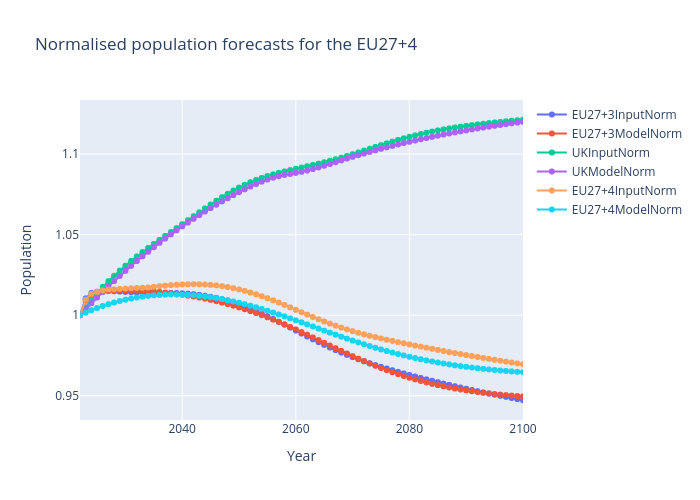
\includegraphics[width=\linewidth]{130quantification/external/population.png}
      \caption{Population projections for the EU27+3 and the UK}\label{fig:population} 
\end{figure}

\subsubsection{EU27 + 4}

\textbf{Data source:}~\cite{eurostat2023population}

\subsubsubsection{Population modelling results:}

The full results of the population modelling are presented in
\autoref{tab:population}.

\subsubsubsection{Highlights:}

\begin{itemize}
      \item The EU population is projected to rise from 446.7 million in 2022, peaking at
            453.3 million in 2026 (+1.5\%), before decreasing to 447.9 million in 2050 and
            further to 419.5 million in 2100.
      \item An increase of 5.8 years is expected in the median age of the EU population
            between 2022 and 2100.
      \item By 2100, the number of individuals aged 80 and over in the EU is projected to
            reach 64.0 million.
\end{itemize}

Populations evolve over time due to demographic factors: births, deaths, and
migration. Each of these factors influences the population's structure.
Presently, the EU is experiencing a trend of ageing in its population due to
the prevailing levels of fertility and mortality.

EUROPOP2023 offers deterministic projections based on `what-if' scenarios.
These scenarios are formed on anticipated courses for fertility, mortality, and
migration. A partial convergence is assumed among the countries in the
EUROPOP2023 projection concerning fertility, mortality, and migration patterns.
The methodology employed is primarily based on past projection exercises.
Furthermore, this study accounts for the impact of the COVID-19 pandemic and
the mass influx due to the conflict between Russia and Ukraine.

It is projected by Eurostat that all EU Member States and the three EFTA
countries will experience continued population ageing. The population in 2100
is predicted to be lower than in 2022, with a decline in the working-age
demographic. There's an observed trend of ageing within the elderly demographic
itself. Migration can both alleviate and accelerate the ageing process. It
depends on whether there's an influx or outflow of the working-age population.
For instance, the search for better job opportunities can lead to a
considerable outflow. Consequently, age dependency ratios are set to rise,
posing challenges for public expenditure on pensions, healthcare, and long-term
care.

\subsubsubsection{Method}

Eurostat provides international projections for the European Union (EU) and the
European Free Trade Association countries, which include Iceland,
Liechtenstein, Norway, and Switzerland. Unlike the UN's projections, Eurostat's
are deterministic in nature. Their most recent projection, dating from 2020,
presents a base variant along with four other variants, starting with the
baseline year 2019. In the base variant, it is forecasted that the EU-27
population will decline by nearly 7 percent or about 30 million people by 2100.
However, in the medium term, the population is expected to grow until 2025,
reaching about 449 million people, before reducing to 416 million by 2100.
Country-specific, sex, and age data are available in Eurostat`s database.

The final projection starts with the 2022 population divided by sex and age.
Mortality rates are applied to determine the number of deaths. Numbers for
non-EU and EU immigrants are computed. For the years 2022 and 2023, refugees
under TP are also included. Emigrants, including refugees under TP for the
years 2024 to 3033, are then subtracted. Based on this, the end-of-year
population and the working-age population are computed. Using these figures,
additional non-EU immigrants are calculated, and the end-of-year population is
re-assessed. This allows for the computation of live births, total deaths,
immigration, and emigration for 2022.

\subsubsubsection{Scenarios}

Eurostat also considers five alternative scenarios besides the baseline for
EUROPOP2023. These are: lower fertility, lower mortality, zero net migration,
decreased non-EU immigration, and increased non-EU immigration. For instance,
the lower fertility scenario posits a total fertility rate that's 20\% less
than the baseline for each projection year (2023 -- 2100). This implies fewer
live births yearly compared to the baseline. The lower mortality scenario
suggests a life expectancy at birth in 2100 that's two years more than the
baseline. Migration scenarios include zero net migration, 33\% less non-EU
immigration each year, and 33\% more non-EU immigration every year throughout
the projection horizon.

\subsubsection{UK}

\textbf{Data source:}~\cite{ons2023population}


\begin{itemize}
      \item New data will be released January 2024.
      \item No scenarios were developed due to the additional uncertainty in the underlying
            data related to the CoViD-19 pandemic-related fluctuations.
\end{itemize}

\subsubsubsection{Population modelling results:}

The full results of the population modelling are presented in
\autoref{tab:population}.

\subsubsubsection{Population Projections}

The UK population in mid-2020 was estimated at 67.1 million. Over the decade to
mid-2030, it's projected to rise by 2.1 million (3.2\% increase), in comparison
to a 6.9\% increase between 2010 and 2020. Over the next 25 years, the
projected growth is 3.9 million (5.8\%), less than the 15.6\% growth between
mid-1995 and mid-2020.

In contrast to the EU27+3, the UK population is projected to continue to
continue growing (slowly) until 2100, the end of the projection period, when it
reaches 76 million.

\subsubsubsection{Assumptions:}
\begin{itemize}
      \item Long-term averages are based on a 22-year period, excluding the 1990s.
      \item Long-term average falls within the ranges given by expert advisory feedback.
      \item Estimated international migration data is used for the years ending mid-2021
            and mid-2022.
      \item Linear interpolation is used from mid-2022 up to mid-2026.
      \item A three-year average of data from mid-2020 to mid-2022 is used for starting the
            linear interpolation for mid-2022.
      \item UK completed family size to reach 1.59 children per woman by 2045.
      \item Annual improvement in UK mortality rates will be 1.2\% for most ages by 2045.
      \item Net international migration to the UK will average +205,000 from mid-2027
            onwards.
\end{itemize}

\subsubsubsection{Methodology}
Projections are produced for successive years from one mid-year to the next. Age-based calculations are made to account for net migration, deaths, and births. Details such as migration timing, death rates, birth rates, and the ratio of male-to-female births are factored into the calculations. Projections are made for each UK country and then aggregated for broader regions.

\subsubsubsection{Strengths and Limitations}
Projections are based on the latest available data but are not forecasts. The inherent uncertainty in the data and the unpredictability of future events means projections may not align with future outcomes. Factors like political and economic changes can also impact population growth, and events like the UK leaving the EU or the COVID-19 pandemic are not explicitly factored in. While this bulletin focuses on projections up to mid-2045, the data includes projections up to mid-2120, which have greater inherent uncertainty.

\subsubsubsection{Merging the EU27+3 and the UK into a unified population model}

As the world undergoes the demographic transition, the relevance of Verhulst's
logistic model has resurged, providing an adequate representation of current
population growth trends. This logistic population growth dynamic is critical
for achieving global sustainable development.

These projections are informed by the finite reserves of primary exhaustible
resources and the ongoing trend of declining birth rates. These indications
suggest a shift towards a new equilibrium state for the planet that aligns with
heightened industrial and technological capacities and improved healthcare
standards. By constructing logistic models that depict the growth dynamics of
the global population and individual continents, we can forecast population
sizes and their growth rates for the next two centuries. The insights garnered
present opportunities for the regulation and optimal management of global
demographic resources.

\subsubsection{Projection Methodology}

\textbf{Methodology source:}~\cite{vanella2020populationprojections}

Population projections underpin many political and economic decisions at
various levels. Often, the users lack the expertise to fully grasp the methods
and limitations of the projections they rely on.

Population development is contingent upon three primary factors: fertility, net
migration, and mortality. Usually, a projection starts with the age- and
sex-specific numbers at a given time. Using estimates for the future
development of the three determinants, the population is projected forward.
Forecasts often refine mortality and migration by age and sex.

Projection methodologies fall into deterministic and stochastic categories.
Deterministic models, being the most widespread, set parameters in one or more
scenarios. Their strengths lie in ease of use, adaptability to changes in
parameters, and straightforwardness for non-experts. A prominent deterministic
method is the cohort component method (CCM) which separately simulates
fertility, migration, and mortality before integrating them into a projection.
Given a population \(P_{t-1}\) at the end of period \(t-1\), the CCM updates
this using births \(B_t\), net migration \(M_t\), and deaths \(D_t\) as:

\[ P_t = P_{t-1} + B_t + M_t - D_t \]

However, deterministic models face challenges. They:
\begin{itemize}
      \item Overlook the probabilistic nature of population processes.
      \item Rely on rigid future assumptions with low individual probabilities of
            occurrence.
      \item Limit the number of considered scenarios, inadequately reflecting future risk.
      \item Lack probabilistic quantification for identified futures.
      \item May be biased by experts' subjective assessments.
\end{itemize}

In contrast, stochastic models view parameters as random variables. While
deterministic models might assume fixed values for determinants like \(G_t,
M_t\), and \(S_t\) in certain scenarios, stochastic models see these as
probabilistic, represented as:

\[ \tilde{B}_t = \tilde{B}_{t-1} + \tilde{G}_t + \tilde{M}_t - \tilde{S}_t \]

Yet, it's essential to understand that no forecast offers absolute truth. Their
aim isn't predicting unexpected events, but extrapolating core demographic
trends. Both deterministic and stochastic methods exist to quantify forecast
uncertainty.

Applying these results in real-world scenarios warrants a cautious approach.
Past trends might not persist in the future. For instance, population growth
isn't just about demographics but also infrastructure. Can a housing market
accommodate growth? Will cities meet their limits? Projections inherently carry
assumptions. For instance, regions must meet housing demands, and urban
challenges arise from positive population growth, such as the need for expanded
childcare or public transport infrastructure.

Predicting and managing future global population growth stands as a paramount
challenge for humanity. Most contemporary researchers believe there's a ceiling
to the planet's `carrying capacity'. Come 2022, Earth's population is
anticipated to hit the eight billion mark. UN predictions suggest that by 2100,
this number will rise to ten billion. However, there's an observable trend
towards smaller family sizes, with birth rates currently hovering around the
replacement rate of 2.1 children per woman. Should global fertility rates align
with family replacement levels (2.0) by 2100, Earth's population is projected
to stabilise between ten and eleven billion. The emergence of new statistical
data necessitates updates to global population growth models. Where once the
Verhulst logistic model was deemed inadequate for characterising global
population growth dynamics, the tapering growth rate now reaffirms its
applicability. Many recent studies have leveraged the logistic growth model.
Our analyses confirm that Earth's population growth rate aligns closely with a
quadratic function, mirroring the Verhulst equation (Fig. 4). All subsequent
computations will employ the Verhulst logistic model:

\begin{equation}
      \frac{dY}{dt} = a \cdot Y - b \cdot Y^2
\end{equation}

The solution to equation (8) will be sought as a logistic function:

\begin{equation}
      Y = g + \frac{b}{1 + A \exp(-a(t - t_0))}
\end{equation}

Function \( Y(t) \) parameters were ascertained using the least squares method,
ensuring maximal alignment between the function's value and the existing
statistical data. The parameter \( g \) was presumed equal to the initial
population size at the start of observations (\( t_0 =1900 \)).

\subsubsubsection{Curve Fitting Explanation}

Terms with subscript 1 describe the initial logistic component, charting
population growth from 2022 to 2042.

Subscript 2 terms Correspond to the second logistic component, which outlines
post-2042 population decline.

\begin{description}[style=nextline, leftmargin=2cm]
      \item[\(\mathbf{b_1}\)] 
            Represents the initial population at the start of the observation period - Europe's population in 1900 per the model's parameters.

      \item[\(\mathbf{b_1}\)] 
            Denotes the carrying capacity of population growth, effectively indicating the population apex achievable via the first logistic function.

      \item[\(\mathbf{A_1}\)] 
            Influences the gradient of the first growth phase. Higher values result in steeper population inclines.

      \item[\(\mathbf{a_1}\)] 
            Represents the growth rate of the initial logistic function, dictating how swiftly the population nears the carrying capacity \( b_1 \).

      \item[\(\mathbf{t_1}\)] 
            Marks the inflection point in the first logistic phase, signifying the period of maximum growth velocity.

      \item[\(\mathbf{b_2}\)] 
            Illustrates the decline's carrying capacity, indicating the population decrease as projected by the second logistic function.

      \item[\(\mathbf{A_2}\)] 
            Determines the gradient of the decline phase, with larger values resulting in sharper declines.

      \item[\(\mathbf{a_2}\)] 
            Represents the rate of decline in the latter logistic function, determining the speed at which the population reaches the decline's carrying capacity \( b_2 \).

      \item[\(\mathbf{t_2}\)] 
            Highlights the inflection point during the decline phase, marking the period where the decrease is most rapid.
\end{description}


\begin{table}[h!]
      \centering
      \small
      \caption{Population projections for the EU27+4}\label{tab:population}
      \begin{tabular}{|C{1.5cm}|C{1.5cm}|C{1.5cm}|C{1.5cm}|C{1.5cm}|}
            \hline
            \rowcolor{headerblue} % Applying the header color
            \textcolor{white}{\textbf{YEAR}} & \textcolor{white}{\textbf{MEDIAN AGE}} & \textcolor{white}{\textbf{EU27+4} (million)} & \textcolor{white}{\textbf{EU27+3} (million)} & \textcolor{white}{\textbf{UK} (million)} \\
            \hline
            \csvreader{csvs/population.csv}{}{\csvcoli& \csvcolii& \csvcoliii& \csvcoliv& \csvcolv\\ \hline}
      \end{tabular}

\end{table}



\clearpage
\subsubsection{Incorporation of demographic factors into individual waste stream models}


\boxws{This section will be filled out with the details of exactly how the demographic parameters are incorporated into your stock and flow models}


\wasteSubsubsubsecBATT
\begin{itemize}
    \item X
\end{itemize}

\wasteSubsubsubsecCDW
\begin{itemize}
    \item X
\end{itemize}

\wasteSubsubsubsecELV
\begin{itemize}
    \item X
\end{itemize}

\wasteSubsubsubsecMIN
\begin{itemize}
    \item X
\end{itemize}

\wasteSubsubsubsecSLASH
\begin{itemize}
    \item X
\end{itemize}

\wasteSubsubsubsecWEEE
\begin{itemize}
    \item X
\end{itemize}


\subsubsection{Conclusion}


\boxreview{This conclusion will be compiled once the individual waste stream sections for each parameter are complete.}


\sectionEndlines
\clearpage

\clearpage
\subsection{Economic factors: \textit{GDP growth}}\label{sec:quantification_economic}

\subsubsection{Definitions}

\begin{description}[style=nextline]
  \item[Gross Domestic Product (GDP) PPP]
        A measure of a country's economic output that accounts for differences in price levels between countries. By using PPPs and the common currency of international dollars, GDP PPP is adjusted for price level differences across countries, providing a more accurate measure of the economic output and living standards, as it reflects the real purchasing power of the citizens.

  \item[Purchasing Power Parity (PPP)]
        An economic theory that allows the comparison of the purchasing power of various world currencies to one another. It involves a comparison of the relative prices of a standard set of goods and services in different countries, thus providing a measure of the relative cost of living and enabling a more accurate comparison of economic well-being.
\end{description}

\boxparameter{GDP growth}{Slow stable growth}{Slow stable growth}{Slow stable growth}



\subsubsection{Sources of data}

The GPD projections for FutuRaM's future scenarios are based on economic data from the OECD as well as population data from Eurostat and the UK's ONS~\cite{oecd2021gdpdata,eurostat2023population,ons2023population}

\subsubsection{Results of projections}

As an `external element', the GDP projections do not differ across the scenarios, only as a function of time.

The results of the projections are shown in~\autoref{fig:gdp-projections}. An interactive figure can be viewed \href{https://futuram-project.github.io/FutuRaM.github.io/WP2/assets.html}{here~\faLink}

\begin{landscape}
\begin{figure}[h!]
    \centering
    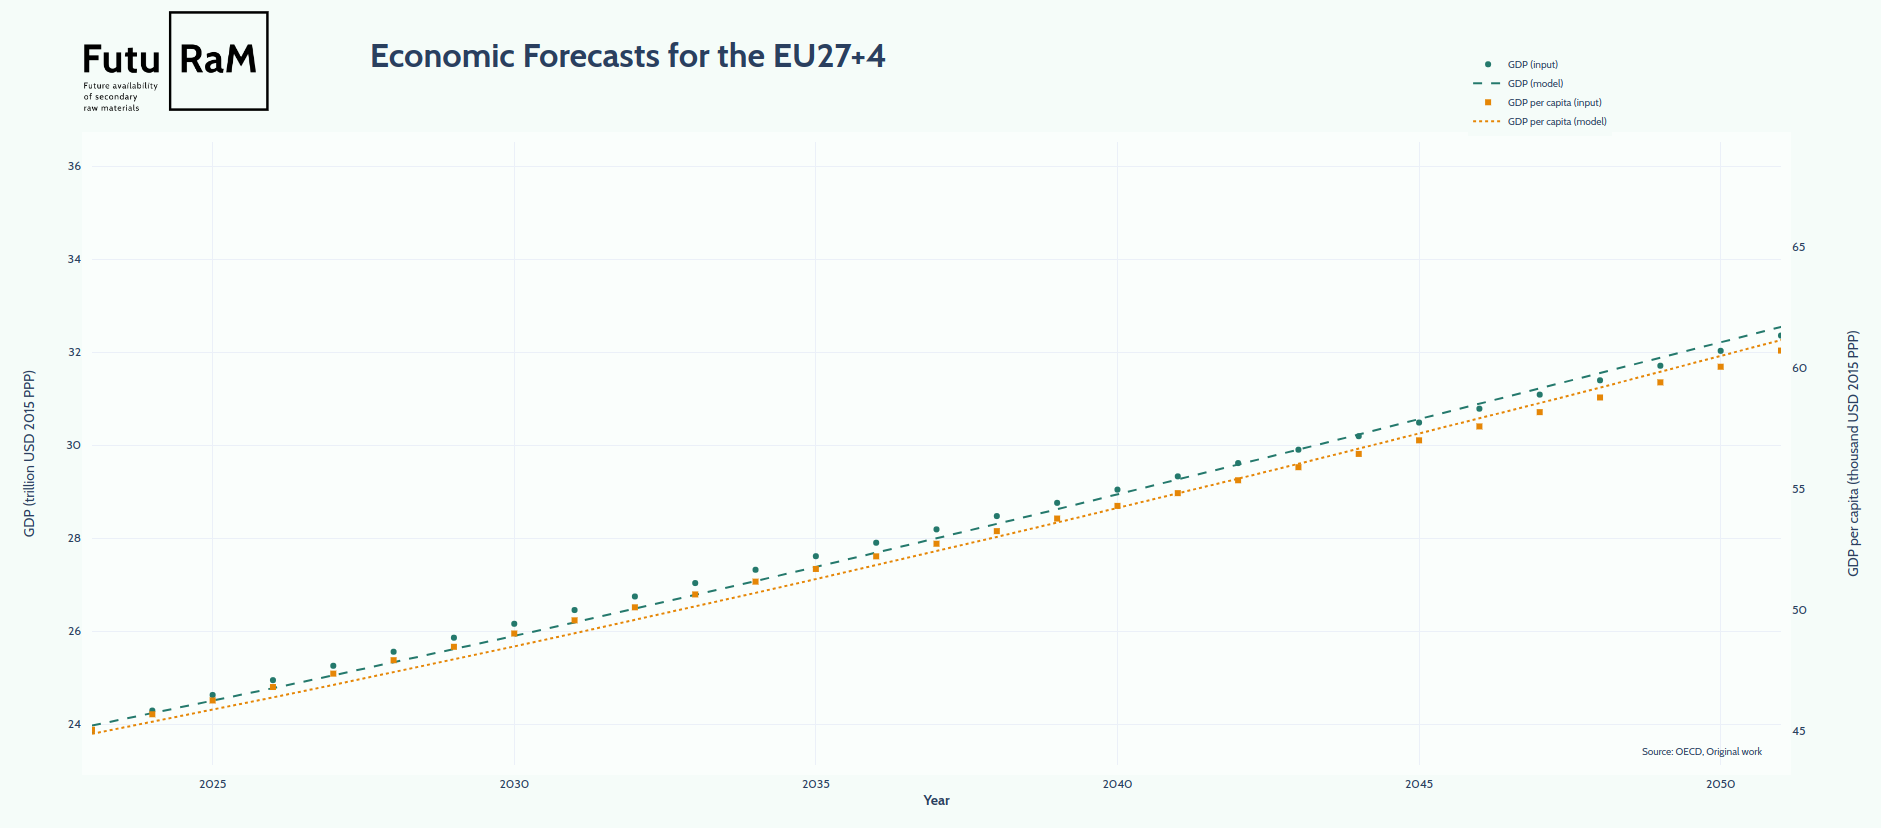
\includegraphics[width=\linewidth]{130quantification/external/gdp.png}
    \caption{GDP projections for the EU27+4}\label{fig:gdp-projections}
\end{figure}
\end{landscape}
\FloatBarrier

\subsubsection{Methodological Overview of OECD's GDP Projection Framework}~\cite{oecd2021gdpdata, oecd2021gdpmethod,duval2010gdp, oecd2012gdp}

The OECD's approach to projecting GDP is rooted in the principle that income levels across various nations will gravitate towards those observed in the most advanced economies, an idea put forth by~\cite{barro2004gdp, barro2004gdpbook}. This convergence is modelled through an enriched version of the Solow growth model, factoring in a dual-sector configuration~\cite{mankiw1992gdp}, which the OECD dubs the ENV-Growth model. Rather than focusing solely on convergence in income, the ENV-Growth model prioritises the growth factors that will drive GDP over time.

For GDP projections up to 2060, the OECD combines model-based assessments with expert evaluations, considering the economic dynamics of individual countries and the global market. These forecasts are denominated in the constant US dollars and PPPs of 2010, based on data from OECD and World Bank, which use the Atlas method for calculating PPPs~\cite{worldbank2023gdp,oecd2021gdpmethod}. The data originate from the OECD Long-Term Baseline Scenario. This scenario, which is integral to the OECD Economic Outlook, serves as a comparative standard to gauge the possible effects of structural reforms, assuming a policy-neutral environment. Conversely, long-term projections diverge from the medium-term forecasting model, which is predominantly demand-driven, by focusing on a supply-side perspective that takes into account labour and capital availability and productivity growth rates.



\subsubsection{Determinants of Long-term Growth}~\cite{fontagne2022gdp, oecd2021gdpmethod}


Recognizing the multifaceted nature of economic advancement, GDP growth projections consider an array of influences such as demographics, educational attainment, technological progress, energy access, and capital flow patterns. The MaGE framework facilitates GDP estimation by charting dynamic paths that reflect the structural interplay defining the economic landscape until 2050~\cite{fontagne2022gdp}.

The ENV-Growth model's projections span a century and include a wider selection of countries, enhancing the original methodologies developed by the OECD Economics Department~\cite{duval2010gdp, oecd2012gdp}. It introduces considerations for energy usage and resource revenue from oil and gas sectors, aligning with the enhanced sectoral approach for fossil fuels presented by~\cite{chateau2012gdp}.


The model's foundation lies in its projection of the five pivotal elements driving economic growth:

\begin{itemize}
  \item Physical capital
  \item Employment, shaped by population trends, age demographics, participation rates, and unemployment scenarios
  \item Human capital, based on education and its consequential effect on labour productivity
  \item Energy demand and resource extraction for exporting countries
  \item Total factor productivity (TFP)
\end{itemize}

The determinants of growth are not restricted to these factors; they also encompass a spectrum of social, economic, and institutional influences, including workforce education, trade openness, institutional integrity, fiscal strategies, regulatory frameworks, and demographic shifts. The underlying potential for economic catch-up through technology transfer and innovation is underscored by the differential in income between each country and the global technology frontrunner.

In the context of employment, projections from IIASA inform the total employment figures, combining time-specific participation rates for different age cohorts with projected unemployment trends. Education assumptions translate gender and age-specific educational projections into a human capital index, which then informs labour productivity enhancements.

For physical capital, the model follows a standard capital accumulation methodology with a set depreciation rate, with the investment rate per unit of GDP edging towards a balanced growth path level determined by the production function's structural parameters.

Energy and natural resources are integrated as productive components for consumers and as extra income from specific oil and gas sectors for producer nations. The model calibrates domestic energy productivity to historical improvement rates, progressing towards an efficiency frontier indicative of cutting-edge energy appliances. The economic contribution of energy resources to producer countries is extrapolated from resource depletion models that describe the dynamics between reserves and resources and the temporal evolution of marginal production costs.

FutuRaM's economic forecasts, while not based directly on the SSP data, are consistent with the SSP2 baseline derived from similar sources and models~\cite{ssp2017narrative, jiang2017ssp, leimbach2017ssp, cuaresma2017ssp, dellink2017ssp, samir2017ssp}, offering a comprehensive picture of potential economic trajectories.


\begin{figure}[h!]
  \centering
  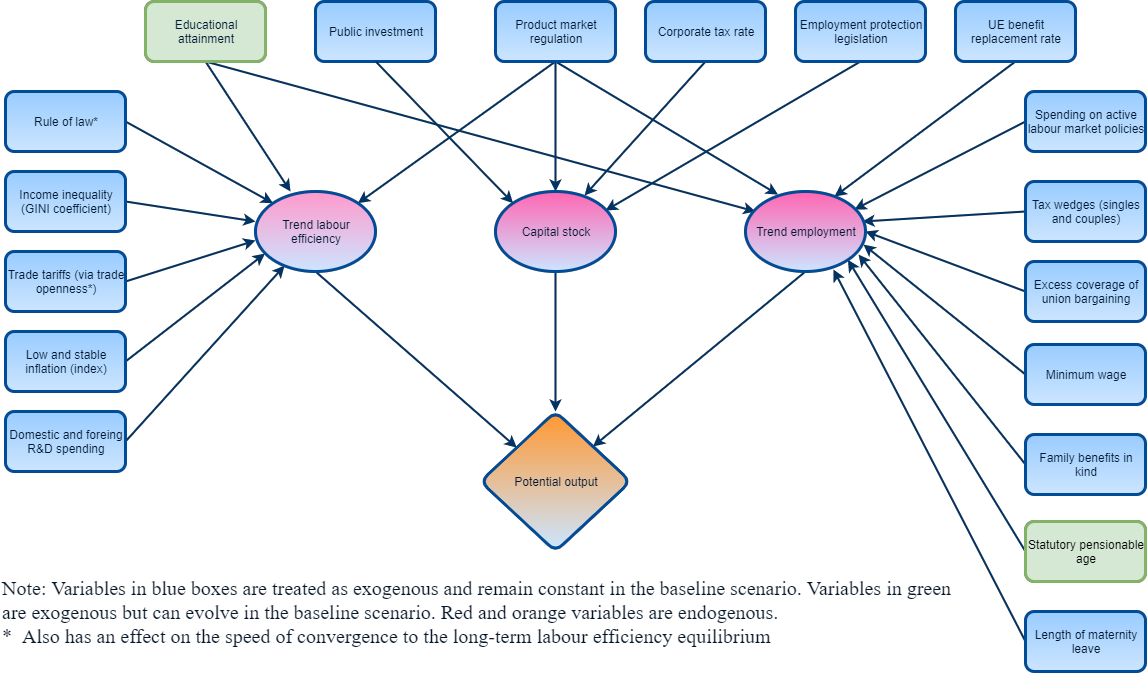
\includegraphics[width=\textwidth]{130quantification/external/oecd2021gdpmethod_drivers.png}
  \caption[Factors incorporated in the long-term GDP model]{Factors incorporated in the long-term GDP model~\cite{oecd2021gdpmethod}}\label{fig:gpd_method}
\end{figure}

\clearpage
\subsubsection{Implications of GDP Growth on FutuRaM's Waste Models}

GDP growth has significant implications for models concerning secondary raw material recovery and waste generation. For example, increasing GDP tends to lead to higher consumption levels, which can result in more waste generation across various streams. However, higher income also provides greater resources for investment in recovery technologies and infrastructure. Below are some examples for each of the specified waste streams.

\wasteSubsubsubsecBATT

As GDP grows, the demand for electronic devices and electric vehicles typically increases, leading to a higher turnover of batteries. This could necessitate advancements in recovery methods for battery components, such as lithium and cobalt, to reduce reliance on primary sources and mitigate environmental impact.

\wasteSubsubsubsecCDW

Economic growth often spurs construction activity, thereby increasing CDW. Increasing GDP as a ratio of waste generation could lead to enhanced recycling processes, promoting the circular economy by converting waste into secondary raw materials for new construction projects.

\wasteSubsubsubsecELV

The number of ELVs rises with economic prosperity, as people can afford newer vehicles more often. This creates opportunities to recover valuable materials and components, necessitating more efficient recycling processes.

\wasteSubsubsubsecMIN

As economies expand, so does the demand for minerals, potentially increasing mining waste. With increased GDP, there could be more investment in techniques to minimise waste generation and recover valuable materials from mining by-products.

\wasteSubsubsubsecSLASH

Higher GDP can correlate with increased industrial activity, producing more slags and ashes. Enhanced recovery techniques can transform these by-products into useful secondary raw materials, such as aggregates in construction.

\wasteSubsubsubsecWEEE

GDP growth can lead to shorter replacement cycles for electronic goods, increasing the amount of WEEE. There's a potential for improved recovery of precious metals and rare earth elements, driving innovation in e-waste recycling technologies.

\clearpage

\subsubsection{Incorporation of economic growth into individual waste stream models}

\boxws{This section will be filled out with the details of exactly how this parameter is incorporated into your stock and flow models}

\wasteSubsubsubsecBATT
\begin{itemize}
    \item X
\end{itemize}

\wasteSubsubsubsecCDW
\begin{itemize}
    \item X
\end{itemize}

\wasteSubsubsubsecELV
\begin{itemize}
    \item X
\end{itemize}

\wasteSubsubsubsecMIN
\begin{itemize}
    \item X
\end{itemize}

\wasteSubsubsubsecSLASH
\begin{itemize}
    \item X
\end{itemize}

\wasteSubsubsubsecWEEE
\begin{itemize}
    \item X
\end{itemize}



\subsubsection{Conclusion}

Economic growth can therefore act as both a driver of waste generation and a catalyst for innovation in the recovery of secondary raw materials. The challenge for models like FutuRaM lies in accurately predicting these trends and proposing effective strategies to balance economic benefits with environmental sustainability.

\boxreview{This conclusion will be more completely compiled once the individual waste stream sections for each parameter are complete.}

\sectionEndlines

\clearpage


\clearpage
\subsection{The Renewable Energy Transition}\label{sec:external-energy_transition}


\subsubsection{Definition}

The term "energy transition" refers to the current global shift from fossil fuels to renewable energy sources to meet the urgent need to reduce greenhouse gas emissions, combat climate change, and enhance energy security. This transition encompasses a fundamental transformation of energy supply and consumption patterns, including the increased use of sustainable energy to achieve a low-carbon economy. Historical shifts in energy sources—from biomass to coal, and later to oil and natural gas—reflect the ongoing evolution of energy use. The present focus is on scaling up renewables such as solar and wind, which are becoming increasingly cost-competitive. Key aspects of the transition include adopting electric vehicles, improving public transportation, advancing energy-efficient technologies for building heating, and developing energy storage and grid solutions to support the integration of variable renewable energy sources.

\subsubsection{Future energy mix in the EU}

The projected electricity mix for the EU is presented in \autoref{fig:energy_mix}. An interactive figure can be viewed \href{https://futuram-project.github.io/FutuRaM.github.io/WP2/assets.html}{here~\faLink}

\begin{figure}[h!]
    \centering
    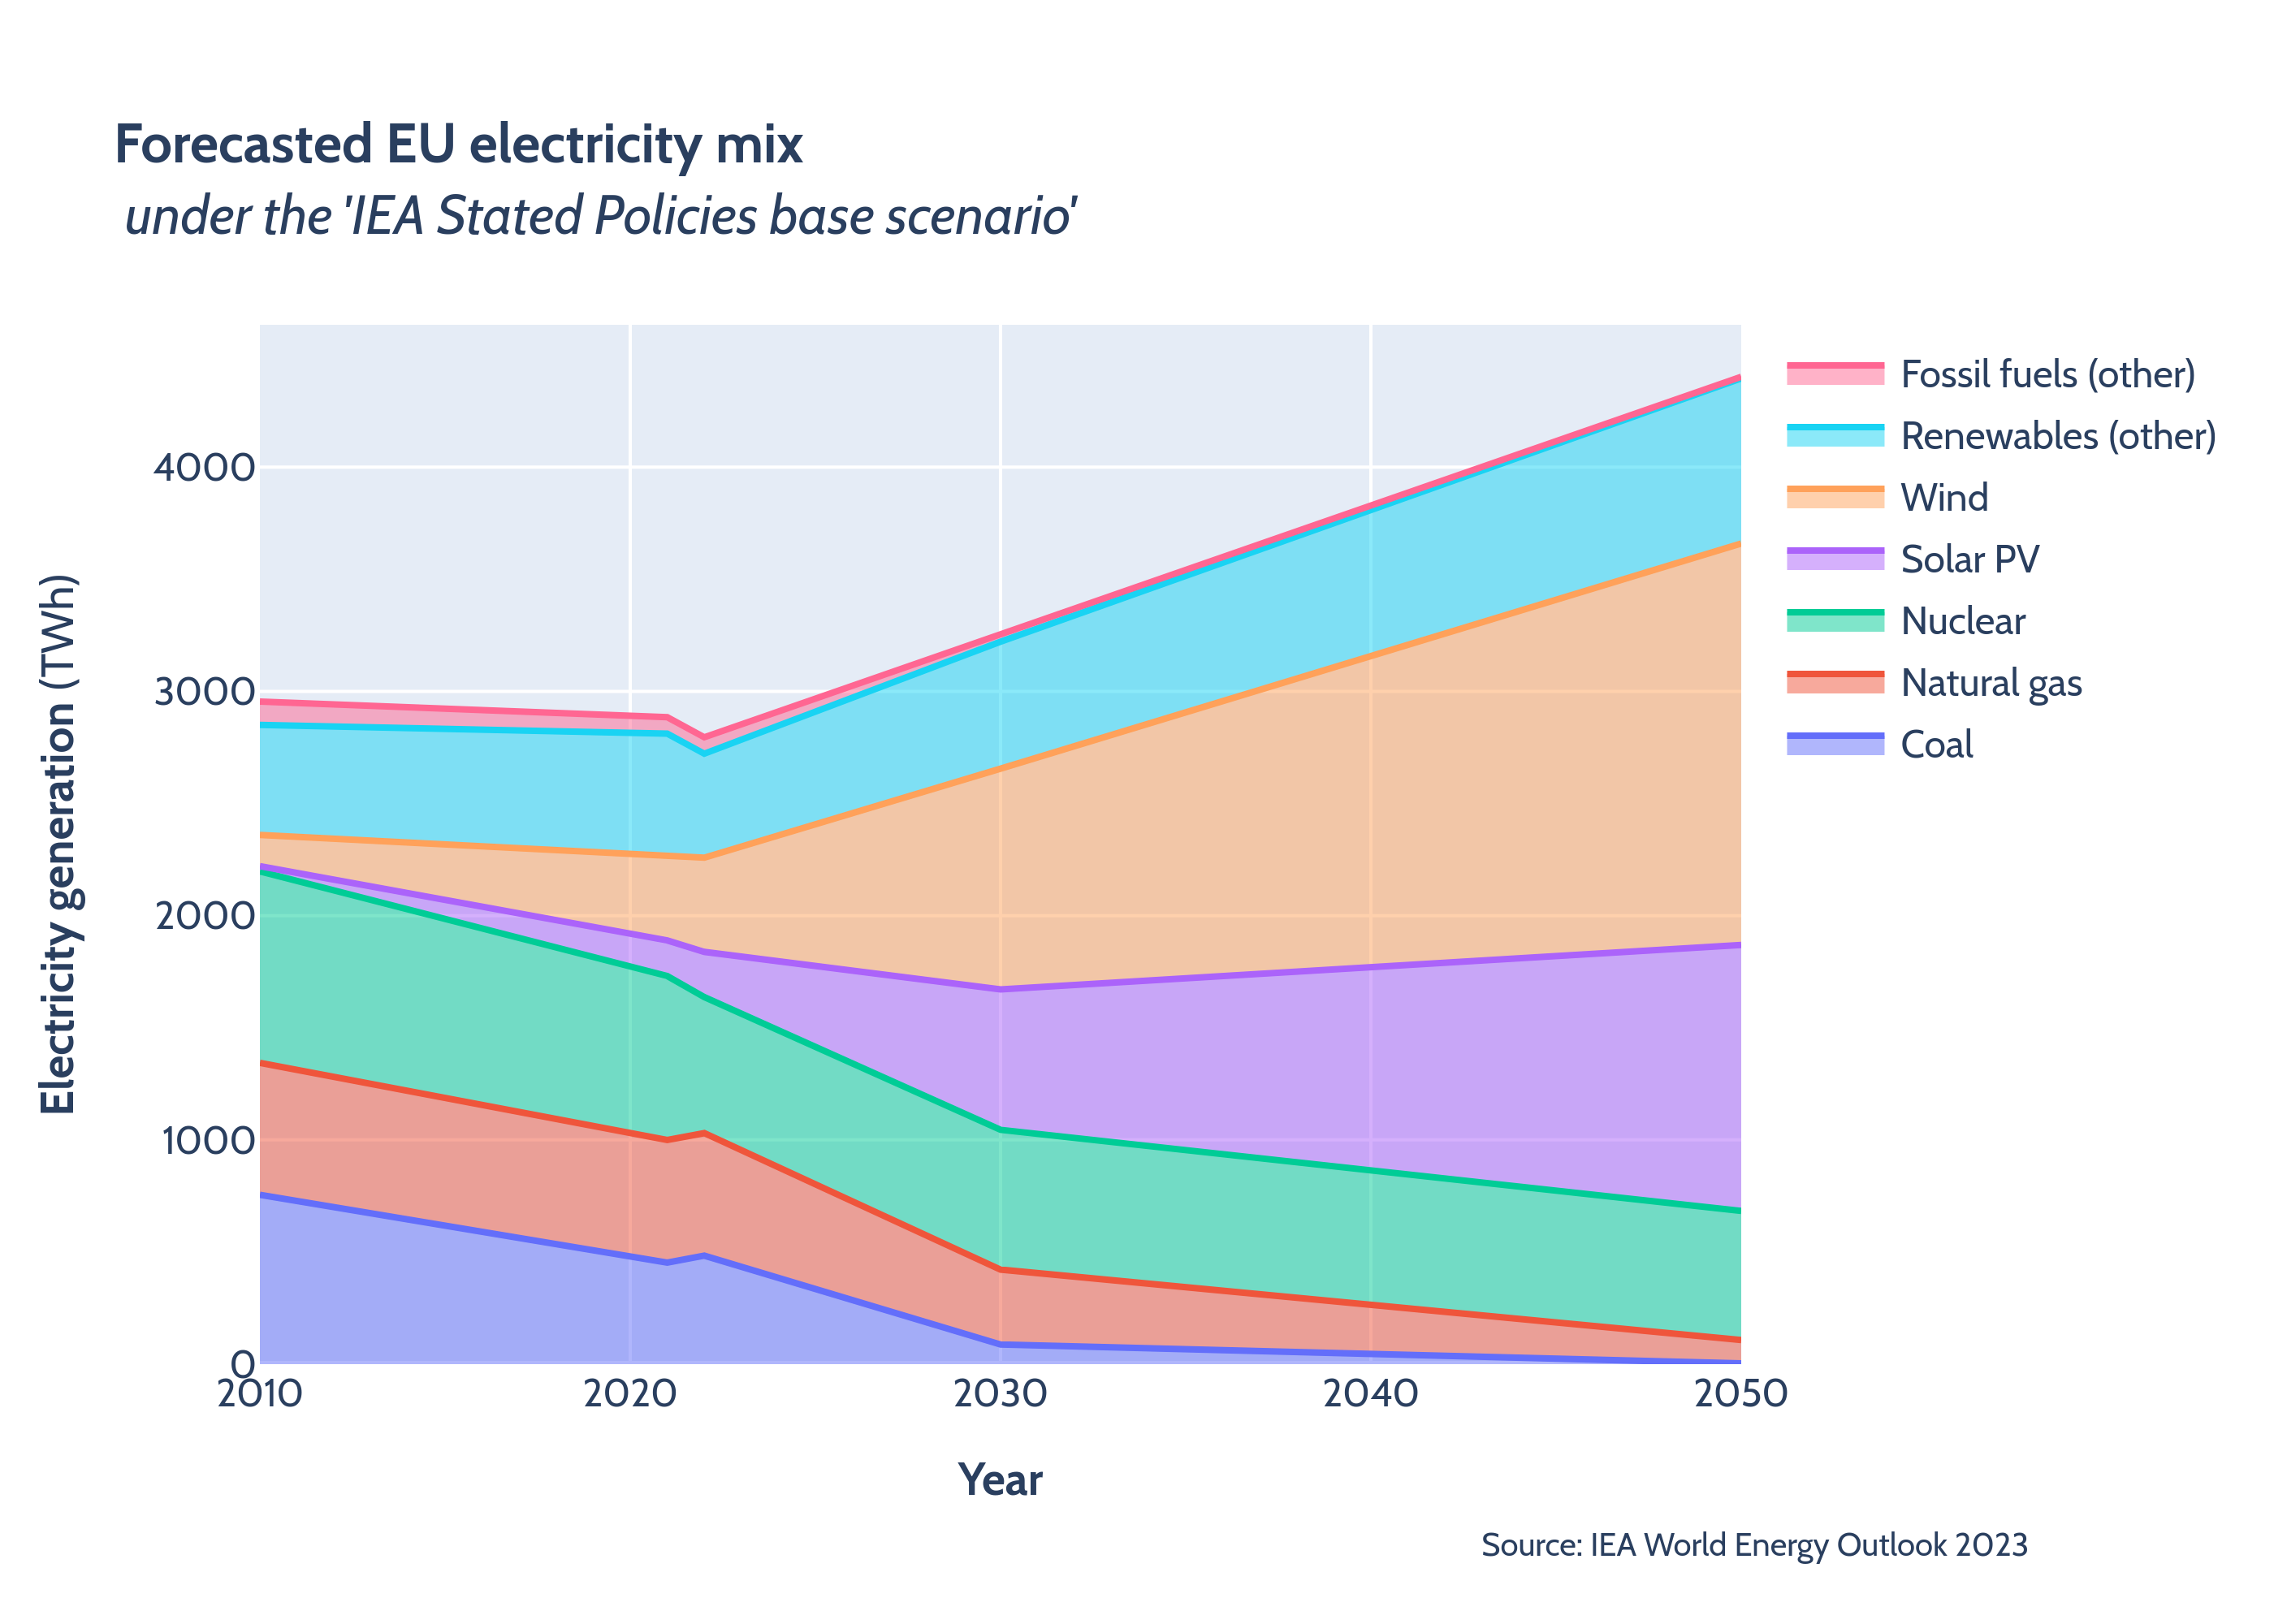
\includegraphics[width=\textwidth]{130quantification/external/energy_mix_forecast.png}
    \caption{EU electricity mix forecast until 2050}\label{fig:energy_mix}
\end{figure}

\subsubsection{Brief context of renewable energy in the EU}

Renewable energy is integral to the EU's shift towards a low-carbon economy and reducing reliance on imported fossil fuels—a response accentuated by the urgency to curtail dependence on Russian energy sources. The EU's strategic move is encapsulated in the REPowerEU Plan of Action, introduced in May 2022, and agreed upon in 2023 which prescribes an aggressive uptake of renewables, emphasizing wind and solar PV, alongside hydrogen, heat pumps, and batteries, vital for energy storage and transportation decarbonisation \cite{jrc2023supplychain,eu2023energy,eu2022repower, jrc2022energyclimateoutlook}.

In analysing the renewable sector in FutuRaM, the focus is on solar PV, wind turbines, electrolysers, batteries, and residential heat pumps. Other renewable sources like bioenergy, hydro, geothermal, and ocean energy, while part of the portfolio, are expected to have minimal impact on critical materials demand and are not central to this analysis.

\subsubsection{Justification for setting as an external scenario factor}

The ongoing global energy transition is a profound shift that holds implications for almost every facet of society, especially regarding CRMs, other raw materials and the system of waste management. This transition from fossil fuels towards renewable energy sources demands a significant increase in various CRMs, influencing their supply and demand curves extensively. In the development of FutuRaM's scenarios, the energy transition is recognised as a fundamental driver of change. However, for the purposes of focussed and strategic scenario modelling, it has been categorised as an external factor.

This classification allows for a delineation between direct policy levers within the purview of SRM systems and broader macro-environmental trends that, while influential, are not the primary subject of analysis within FutuRaM. As such, the project's scenarios incorporate a consistent baseline projection of the energy transition's effects, shared across the three scenarios, ensuring that the core analysis remains centred on material-centric policy outcomes and targets of the CRM act. This ensures that the resulting insights are actionable and tailored to the nuances of material management and recycling systems. It reflects a strategic choice to maintain scenario tractability and avoid the dilution of policy implications that could arise from an overly broad scope of variables.

Moreover, the scenario architecture within FutuRaM is constructed with inherent flexibility, permitting later incorporation of amendments to the background energy transition trends. This adaptability is essential to ensure that, as the energy landscape evolves and new data becomes available, the scenarios can be revised and updated, thereby preserving the relevance and accuracy of the project's findings over time.


\subsubsection{Relevant technologies in the renewable energy sector}

The cornerstone technologies in renewable energy—batteries, electrolysers, wind turbines, heat pumps, and solar PV—play pivotal roles across various sectors (Figure 85). Heat pumps serve industrial processes, while solar PV and batteries support ICT, defence, and mobility with energy and uninterrupted power supplies, respectively \cite{jrc2023supplychain}.

Wind energy, expected to surge, will benefit from cost-efficient, innovative turbines designed for increased productivity in offshore and low-wind conditions. Projections from GECO present two scenarios: a conservative estimate shows wind capacity expanding from 732 GW (2020) to 1,400 GW (2030), and to 4,050 GW by 2050. An optimistic forecast anticipates a rise to 2,500 GW by 2030 and 8,400 GW by 2050.

Solar PV is poised for exponential growth due to advancements enhancing efficiency and lowering costs. GECO's cautious scenario predicts growth from 710 GW (2020) to 2,950 GW (2030), reaching 7,500 GW by 2050. The optimistic scenario projects a tenfold increase by 2030 and sixteenfold by 2050 compared to 2020 levels.

Addressing the intermittency of wind and solar power necessitates adequate storage solutions and robust grid systems, with electrolysers emerging as a crucial technology for renewable hydrogen production, forecasted to exceed 1 GW capacity by the end of 2022 \cite{iea2022renewables}.

Additionally, digitalisation, robotics, and 3D printing are set to boost the renewable sector's productivity and optimisation across its value chain. Heat pump sales are also on an upward trend, with a peak expected in 2045, ranging between 15 million (low demand) and 38 million units (high demand) by 2050.

Material demand in the renewable sector is dominated by wind turbines, electrolysers, and solar PV, with wind energy leading in consumption of critical materials.


\subsubsection{Supply Chain bottlenecks in renewable energy}

Supply chain bottlenecks present a significant challenge in the deployment of renewable energy technologies, particularly for wind turbines, solar PV, electrolysers, and heat pumps. The production of NdFeB permanent magnets for wind turbines demands rare earth elements (REEs) like neodymium, dysprosium, praseodymium, and terbium, with the EU being highly dependent on imports for both raw and processed materials such as permanent magnet alloys and components like blades.

Solar PV technologies necessitate strategic raw materials, including silicon metal and rare metals like gallium and germanium, with China dominating the production of silicon ingots and wafers. This reliance on imports extends across the value chain, including the crystalline silicon cell production where the EU's contribution is minimal.

The battery industry utilizes strategic raw materials such as lithium, manganese, and cobalt, with raw materials and components largely imported. A shift is anticipated towards nickel-rich batteries or alternative chemistries to reduce reliance on high-cobalt-content lithium-ion batteries (LIBs) due to the oligopoly control of critical components in Asia.

Electrolysers for hydrogen production use a range of strategic raw materials, particularly from the platinum group metals (PGMs), but also silicon metal, aluminium, copper, and magnesium, with the EU facing challenges in sourcing these materials. For heat pumps, strategic raw materials needed include magnesium and copper, but no significant bottlenecks have been identified, with most critical materials used in microchips and IT controllers.

Across all technologies analysed, a common pattern of heavy reliance on imports, particularly from China, is observed at different stages of the value chains. The EU’s primary sourcing and processing capabilities for critical raw materials are notably low, creating dependencies at multiple levels. Despite a strong manufacturing capacity for wind turbine assembly, the EU is entirely reliant on imports for the value chain of rare-earth permanent magnets. Similarly, for solar PV, the dependence on imports is comprehensive. The recent surge in Chinese manufacturing market share for heat pumps and the developing value chain for batteries in the EU are also noteworthy.

A breakdown of the materials required for each technology is given in \autoref{tab:energy-crms}.


\newgeometry{left=2cm,right=2cm,top=2cm,bottom=2cm}
\begin{landscape}
    \centering
    \small
    \renewcommand{\arraystretch}{0.8} % adjust the value as needed
    \begin{longtable}{|C{2cm}|L{3cm}|C{2cm}|C{2cm}|C{2cm}|C{2cm}|C{2cm}|C{2cm}|}
        \caption{Raw materials essential to the renewable energy sector}\label{tab:energy-crms}\\
        \hline
        \rowcolor{headerblue} % Applying the header color
        \color{white}\textbf{SUPPLY RISK} & \color{white}\textbf{MATERIAL} & \color{white}\textbf{CRM} & \color{white}\textbf{BATT} & \color{white}\textbf{H2} & \color{white}\textbf{WIND} & \color{white}\textbf{SOLAR (PV)} & \color{white}\textbf{HEAT PUMPS} \\
        \hline
        \endfirsthead%
        \hline
        \multicolumn{8}{r}{\textcolor{headerblue}{\textit{{Continued on next page}}}}\\
        \endfoot%
        \rowcolor{white}
        \multicolumn{8}{c}{{\textcolor{headerblue}{\textit{\tablename\ \thetable{} --- Continued from previous page}}}}\\
        \hline
        \rowcolor{headerblue} % Applying the header color
        \color{white}\textbf{SUPPLY RISK} & \color{white}\textbf{MATERIAL} & \color{white}\textbf{CRM} & \color{white}\textbf{BATT} & \color{white}\textbf{H2} & \color{white}\textbf{WIND} & \color{white}\textbf{SOLAR (PV)} & \color{white}\textbf{HEAT PUMPS} \\
        \endhead%
        \bottomrule
        \endlastfoot%
        \csvreader[separator=comma, late after line=\\]{csvs/energy-crms.csv}{}{
            \csvcoli & \csvcolii & \csvcoliii & \csvcoliv & \csvcolv & \csvcolvi & \csvcolvii & \csvcolviii
        }
    \end{longtable}
    \renewcommand{\arraystretch}{1} % reset \arraystretch to its original value
    \end{landscape}
\restoregeometry% restore margins to normal


The integration of the energy transition has significant implications for the management of Critical Raw Materials (CRMs) across various waste streams due to changing material requirements and waste profiles~\cite{jrc2023supplychain,jrc2020reedemanddata,iea2023energytechperspectives,iea2023crm}.

\vspace{\baselineskip}
\textbf{For example:}

\wasteSubsubsubsecBATT
\vspace{-1cm}
\begin{itemize}
    \item Increased deployment of Li-ion batteries for energy storage will lead to a surge in waste batteries, necessitating improved recycling technologies to recover CRMs.
    \item The transition to renewable energy sources may lead to changes in the battery composition, affecting recycling processes and the types of CRMs that need to be managed.
\end{itemize}

\wasteSubsubsubsecELV
\vspace{-1cm}
\begin{itemize}
    \item The shift towards electric vehicles will transform the composition of ELVs, increasing the relevance of CRMs used in electric powertrains and batteries.
    \item This transition requires the adaptation of ELV recycling infrastructure to efficiently process and recover new types of CRMs.
\end{itemize}

\wasteSubsubsubsecWEEE
\vspace{-1cm}
\begin{itemize}
    \item As energy systems become more digitized and interconnected, WEEE will contain a broader array of CRMs, prompting the need for more sophisticated recycling methods.
    \item The growing volume of WEEE will challenge current recycling capacity and technology, calling for significant innovation in CRM recovery techniques.
\end{itemize}

\wasteSubsubsubsecCDW
\vspace{-1cm}
\begin{itemize}
    \item Green building materials and energy-efficient technologies may introduce new CRMs into CDW, changing the material recovery landscape.
    \item The promotion of deconstruction over demolition could preserve the integrity of materials containing CRMs, allowing for better recovery rates.
\end{itemize}

\wasteSubsubsubsecMIN
\vspace{-1cm}
\begin{itemize}
    \item The drive for clean energy technologies is expected to increase the mining of specific CRMs, potentially leading to higher volumes of mining waste that must be managed sustainably.
\end{itemize}

\wasteSubsubsubsecSLASH
\vspace{-1cm}
\begin{itemize}
    \item The energy transition could increase the generation of certain industrial wastes such as slags, which may contain valuable CRMs.
\end{itemize}

\vspace{\baselineskip}
\subsubsection{Implementation in EU Law}

\subsubsubsection{Fit for 55 Package (2021)}

The "Fit for 55" package is a collection of policy initiatives proposed by the European Commission in July 2021 aimed at revising and updating EU legislation to reflect the increased ambition of reducing net greenhouse gas emissions by at least 55\% by 2030, compared to 1990 levels~\cite{eu2021fitfor55}. This target was a significant step up from the previous goal of a 40\% reduction and is part of the European Union's plan to become climate-neutral by 2050 --- an objective set out in the European Green Deal\cite{eu2019greendeal}.

The package includes proposals to revise the EU Emissions Trading System (ETS), to increase the use of renewable energy, to improve energy efficiency, and to implement carbon pricing mechanisms, among other measures. The intention is to align existing laws with the 2030 climate target and to set the legal foundation for Europe's transition to a green economy. This includes changes across various sectors including transportation, building, and energy production to reduce emissions and promote sustainable practices.

\subsubsubsection{REPowerEU Plan (2022)}

The invasion of Ukraine by Russia has caused significant disruption to energy markets in Europe and globally. To eliminate reliance on an unreliable supplier, the European Commission has devised the REPowerEU plan~\cite{eu2022repower}. This initiative focuses on energy conservation, the production of clean energy, and the diversification of energy sources, supported by financial and legal measures to develop Europe's necessary new energy infrastructure and systems.

\paragraph{Accelerating Clean Energy} Renewable energy sources, being both cost-effective and environmentally friendly, can be produced locally, thereby reducing dependency on imported energy. The REPowerEU plan aims to expedite the green transition and trigger substantial investments in renewable energy. It also seeks to facilitate the rapid transition of industry and transport from fossil fuels, reducing both emissions and dependency.

This includes a variety of measures focused on renewable energy and energy efficiency, such as:

\begin{itemize}
    \item Increasing the EU's 2030 renewable energy target of the `Fit for 55 package' from 40\% to 45\%.
    \item Accelerating the deployment of photovoltaic (PV) energy.
    \item Introducing the European Solar Rooftop Initiative.
    \item Doubling the deployment rate of individual heat pumps.
    \item Decarbonising the industry by promoting electrification and renewable hydrogen.
    \item Speeding up renewable energy project and grid infrastructure permit processes.
    \item Increasing the EU’s binding energy savings target for 2030 to 13\%.
\end{itemize}

The May 2022 REPowerEU plan by the European Commission, in response to the energy market disruptions due to Russia's invasion of Ukraine, is designed to rapidly cut down on the EU's reliance on Russian fossil fuels. It raises the renewable energy target of the Fit for 55 package from 40\% to 45\%.

This ambitious goal for renewable energy use, coupled with REPowerEU’s strategies to reduce energy demand, necessitates substantial increases in renewable capacity across the electricity, transport, and heating and cooling sectors. The Commission forecasts that to meet the 2030 objectives, renewable electricity should reach 69\%, 32\% in transport, and a yearly growth of at least 2.3 percentage points in heating and cooling.


\subsubsubsection{Renewables Energy Directive (2023)}

The recent legislation strengthening the EU Renewable Energy Directive marks an advancement towards the European Green Deal and REPowerEU ambitions. With the provisional agreement, the EU's binding renewable energy target for 2030 is now at least 42.5\%, aiming potentially to reach 45\%. This target significantly surpasses the previous goal of 32\% and is nearly double the present proportion of EU renewable energy.

A distinct enhancement over the REPowerEU plan is the establishment of definitive binding targets for renewable energy. The legislation optimises permitting procedures, acknowledges renewable energy as an overriding public interest, and designates acceleration zones for expedited development in strategically identified regions.

The directive also introduces specific directives across various sectors:

\begin{itemize}
    \item In heating and cooling, it sets forth progressive annual renewable targets and a 49\% renewable energy consumption benchmark in buildings by 2030.
    \item It for the first time includes the industrial sector under its ambit, establishing indicative and binding targets for the use of renewable energy and renewable hydrogen, respectively.
    \item For the transport sector, it specifies a reduction in greenhouse gas intensity and sets sub-targets for advanced biofuels and renewable fuels of non-biological origin, underpinning the EU's renewable hydrogen objectives.
    \item It further enhances the "guarantees of origin" system to improve consumer information and supports the integration of the energy system through electrification and waste heat capture.
\end{itemize}

In summary, the agreement accelerates the EU's strides towards energy autonomy, promises to reduce energy costs over time, and decreases dependence on imported fossil fuels. It intensifies the EU's pledge to a decarbonised economy and aligns with REPowerEU's broader goals but with specific, more ambitious targets and refined processes for rapid renewable energy adoption.

While the reinforced EU Renewable Energy Directive is a pivotal step towards the EU's "Fit for 55" framework and the overarching European Green Deal goals, it has not been without its critics. The Directive's ambitious targets for 2030 have spurred a range of responses from member states and institutions, with concerns centered around feasibility, economic impact, and the varying capabilities of nations to meet these objectives~\cite{eu2023energycritique}.

The following is a summary of the key points raised by member states and the European Commission in their statements on the directive~\cite{eu2023energycritique}:

\begin{description}[style=nextline]

    \item[Belgium] Belgium supports the directive while voicing \textit{"serious concerns"} over the feasibility of increased renewable energy targets, citing \textit{"demographical and geographical limitations"} and the presence of energy-intensive industries. The national contributions and sectoral sub-targets are deemed \textit{"extremely difficult to achieve"} and potentially \textit{"unachievable"} within the proposed timeline.

    \item[Poland] Poland boasts a rapidly growing renewable sector but cannot support the proposed directive, stating it is unrealistic and could destabilize the energy grid and security. They assert that the targets lack realism and flexibility, and stress that the energy transition should be \textit{"accessible to society"} and in favor of European industry.

    \item[Romania] Romania is committed to decarbonisation but expresses concern that the high level of ambition may lead to increased costs and discourage certain sectors, making them \textit{"un-competitive."} They highlight the importance of national specificities and energy mixes in setting targets and advocate for technology neutrality.

    \item[Slovak Republic] Slovakia finds the EU RES target for 2030 \textit{"very ambitious"} and difficult, stressing that additional contributions may not reflect the real potential for renewable development in the country. The statement also points to concerns over hydrogen production support not being satisfactorily addressed.

    \item[European Commission] The Commission acknowledges the significant efforts required from Member States to meet the targets, noting the high adaptation costs for certain industries. It concedes that achieving the directive's objectives will involve significant public and private investment and national budget implications. The Commission emphasizes the need for complementary decarbonisation efforts involving other non-fossil energy sources.

\end{description}

\subsubsection{Challenges to the expansion of renewable energy in the EU}

In addition to the internal conflict among member states~\cite{eu2023energycritique}, a recent IEA analysis concluded that EU's renewable energy expansion is constrained by inadequate policy support, complex permitting, and grid upgrades' pace.~\cite{iea2022renewables}

Current forecasts indicate that the solar PV and wind capacity expansions fall short of the REPowerEU plan's renewable electricity targets for 2030. The European Commission Staff Working Document states that achieving a 69\% share of renewable electricity requires 592 GW of solar PV and 510 GW of wind by 2030, translating to annual additions of 48 GW for solar PV and 36 GW for wind~\cite{eu2022repowerWD}. 

These figures significantly exceed the IEA's main case projections of 39 GW for solar PV and 17 GW for wind between 2022 and 2027, resulting in a renewable generation share of 54\% in the electricity sector—15 percentage points below the desired 69\% by 2030. 

Therefore, to fulfill the necessary installed capacity for generating 69\% of electricity from renewables by 2030, the annual net additions for solar PV need to increase by 22\%, and for wind, more than double~\cite{iea2022repower}. The EU estimates that the total amount required for these investments will exceed €360bn before 2030~\cite{eu2022repowerWD}.


\begin{description}[style=nextline]
    \item[Policy Support:] Uncertainty from infrequent auctions and limited visibility hampers utility-scale solar PV and distributed PV projects, with issues in current auction designs and support scheme extensions affecting growth and profitability.
    \item[Permitting:] A primary bottleneck due to complex regulations, land restrictions, social opposition, and permitting office inefficiencies increases costs and extends project lead times.
    \item[Grid Congestion:] Insufficient grid capacity and upgrade challenges caused by permitting hurdles, labour shortages, and opposition slow the integration of new renewable plants.
\end{description}

The IEA analysis states that improvements addressing these issues could boost solar and wind deployment by 30\% by 2027. An accelerated case requires increased policy support, regulatory reforms, and quicker infrastructure development~\cite{iea2022repower}.

For utility-scale solar PV, competitive auctions must be introduced or extended, with revised auction designs to reflect current market conditions. Distributed PV could see growth with better support and remuneration for self-consumption.

Despite potential policy and regulatory advances, wind energy, particularly onshore, faces persistent permitting difficulties, and offshore wind is bogged down by grid connection delays.

Finally, market interventions and the energy crisis debate could influence renewable investments, stressing the need for careful reform processes involving all stakeholders to maintain investor confidence.

\clearpage
\subsubsection{Incorporation of the energy transition into the FutuRaM scenarios}

\boxreview{There will need to be a discussion about choice of energy scenario and the use of this data: \\ (1) if it is to be used commercially, we will need a license from the IEA; \\ (2) more detailed data is available for purchase \\ (3) the choice of scenario and alignment with the WSs. \\ There are alternatives, such as the EU reference scenario~\cite{eu2020scenarioreference} and the POTEnCIA central scenario, which is similar, although somewhat outdated~\cite{jrc2019scenarioenergy}}


In light of the information presented above, as well as the nature of the three scenarios, FutuRaM will use a moderate growth scenario for the energy transition. The data for this is sourced from the projections of the International Energy Agency (IEA) using the "base case" of their "Stated Policies (STEP)" scenario~\cite{iea2022worldenergyoutlookdata}.

The IEA's World Energy Outlook 2023 presents a range of scenarios, including the Stated Policies (STEP) scenario, the Sustainable Development Scenario (SDS) --- which is the IEA's pathway to achieving the Paris Agreement goals --- and the Net Zero Emissions scenario. Full details of the scenarios are available in the documentation of the IEA's Global Energy and Climate (GEC) Model~\cite{iea2023model}.

A comparison of the IEA's projections for the renewable energy transition in the EU under the STEP and APS scenarios is presented in \autoref{tab:iea_energy_data}.

\begin{table}[h!]
    \centering
    \small
    \caption{Normalized renewable energy supply in the EU using the year 2010 as a base reference}
    \label{tab:iea_energy_data}
    \begin{tabular}{lccc}
        \hline
        Year & Historical & Stated Policies & Announced Pledges \\
        \hline
        2010 & 1.00       & --              & --                \\
        2021 & 1.66       & --              & --                \\
        2022 & 1.66       & --              & --                \\
        2030 & --         & 3.33            & 3.69              \\
        2050 & --         & 5.69            & 7.23              \\
        \hline
    \end{tabular}
\end{table}

A summary of the IEA's scenarios is presented in \autoref{tab:GECscenarios}.

\begin{table}[h!]
    \centering
    \small
    \caption{Definitions and Objectives of the GEC Model 2023 Scenarios}\label{tab:GECscenarios}
    \begin{tabular}{p{4cm}p{3.5cm}p{3.5cm}p{3.5cm}}
        \hline
                             & \textbf{Net Zero Emissions by 2050 Scenario}                                                                                                                             & \textbf{Announced Pledges Scenario}                                                                                                                  & \textbf{Stated Policies Scenario}                                                                                                             \\
        \hline
        \textbf{Definitions} & A pathway to achieve net zero CO2 emissions by 2050 within the energy sector, updated fully in 2023. Universal access to electricity and clean cooking achieved by 2030. & Assumes all climate pledges as of end of August 2023, including NDCs and net zero targets, are met on time.                                          & Reflects energy-related policies in place or under development as of end of August 2023 and planned capacities for clean energy technologies. \\
        \hline
        \textbf{Objectives}  & To detail sector-specific actions needed to achieve net zero energy-related CO2 emissions by 2050 and other sustainable development goals.                               & To assess how current pledges align with the 1.5 °C global warming limit, showing the ambition gap and the steps needed for universal energy access. & To benchmark the achievements and limitations of current policies, highlighting the gap in implementation to meet decarbonisation targets.    \\
        \hline
    \end{tabular}
\end{table}

\subsubsubsection{The Stated Policies Scenario (STEP)}

The Stated Policies Scenario (STEPS) is an energy model that offers a conservative projection based on existing and developing energy policies, without assuming full achievement of governments' announced goals. It undertakes a detailed, sector-by-sector assessment including a variety of factors such as pricing, efficiency standards, and infrastructure projects as of the end of August 2023. 

Although it incorporates far-reaching governmental targets, such as net zero emissions and complete energy access, these are not presumed to be fully implemented without evaluating the regulatory, financial, and infrastructural context of each country.

The STEPS assumes that current time-bound policies will be continued with similar measures but does not speculate on the future intensification or reduction of policies unless there is evidence to suggest this. For the first time in 2023, it also accounts for industry actions, such as the manufacturing capacities for clean energy technologies and their market impact.

Overall, the STEPS indicates that while existing commitments can make a substantial impact, there remains a significant gap to reach the ambitions of the Announced Pledges Scenario or the Net Zero Emissions by 2050 Scenario.

\clearpage
\subsubsubsection{The Future Energy Mix in the EU}

In a global sense, the energy transition manifests in FutuRaM's forecasts by way of the background energy mix. In \autoref{fig:energy_mix} is the IEA's projection of the energy mix in the EU for the Stated Policies scenario. Additional forecasts for rare earth elements (REEs) supply and demand related to wind energy and e-mobility are offered by the JRC~\cite{jrc2020reedemanddata}.

\subsubsubsection{Impact of the energy transition on the FutuRaM scenarios}

\boxreview{--- Many more details to be added later once we have confirmed the scenario choice and the alignment with the WSs \\ --- One advantage of the IEA data is that it is aligned with other data sets, such as CRM supply and demand forecasts \\
--- The figures below are just an example of some of the impacts that we could portray here. Better figures will be generated later.
}



\vspace{2cm}

\textbf{The following figures illustrate some of the impacts that scenario choice can have on raw material demand forecasts~\cite{iea2023crm}}

\begin{figure}[h!]
    \centering
    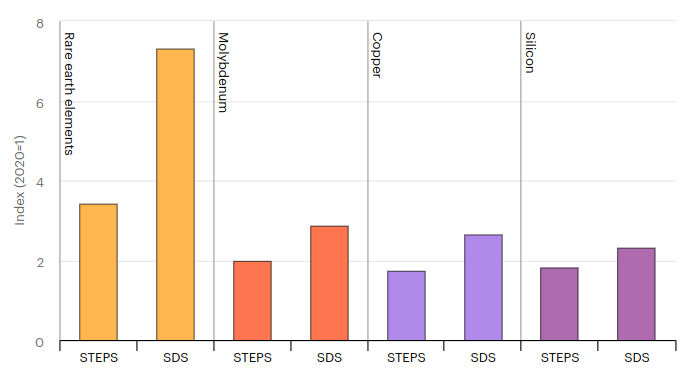
\includegraphics[width=\textwidth]{130quantification/external/energy_change_demand.png}
    \caption{Change in demand for selected elements}\label{fig:energy_change_demand}
\end{figure}

\begin{figure}[h!]
    \centering
    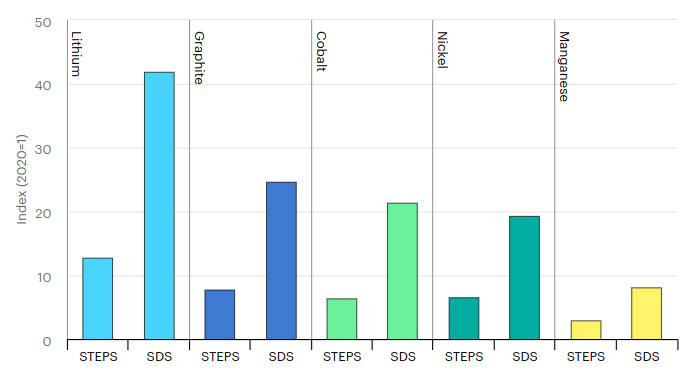
\includegraphics[width=\textwidth]{130quantification/external/energy_change_batt_demand.png}
    \caption{Change in demand for battery relevant elements}\label{fig:energy_demand_batt}
\end{figure}

\begin{figure}[h!]
    \centering
    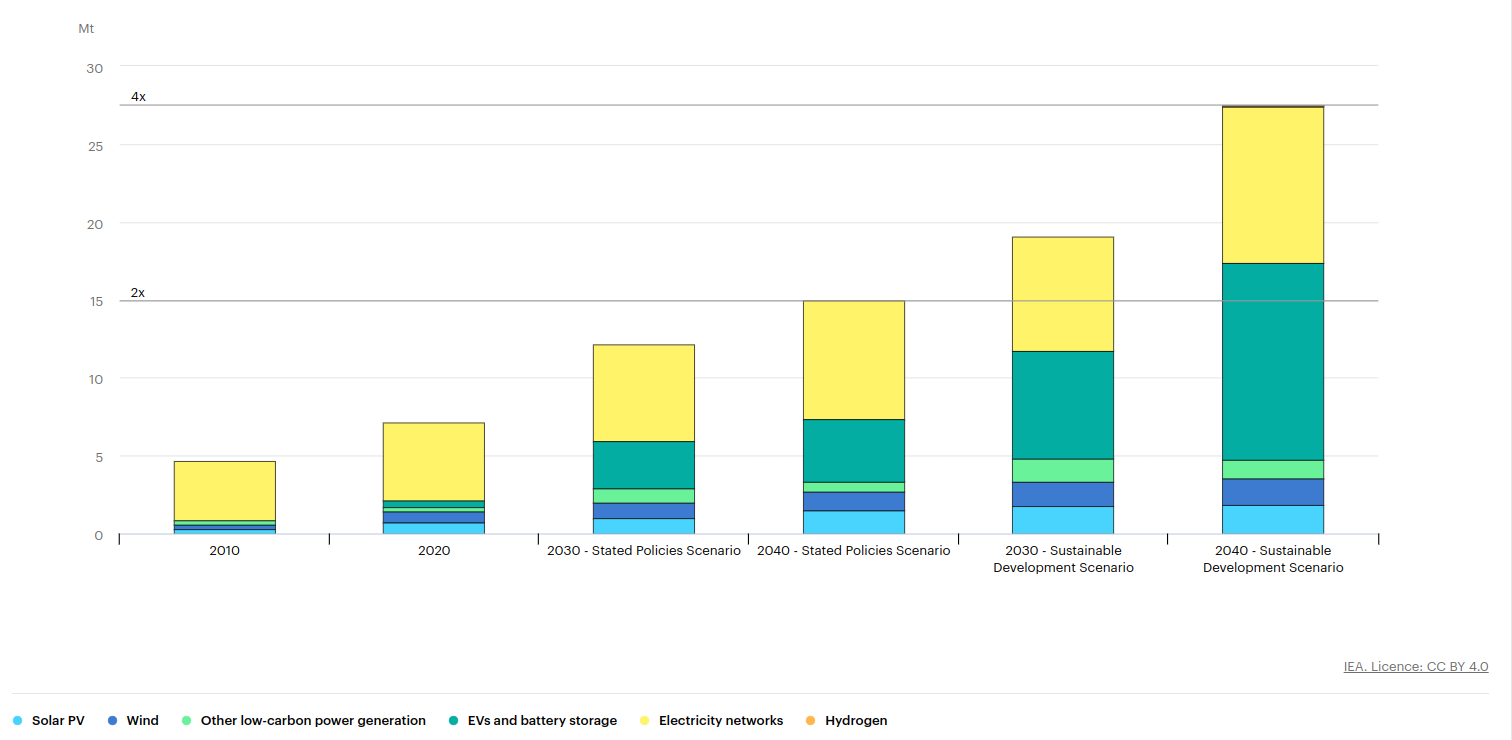
\includegraphics[width=\textwidth]{130quantification/external/energy_total_demand.png}
    \caption{Global mineral demand (total) under various scenarios}\label{fig:energy_mineral_total}
\end{figure}

\subsectionEndline
\clearpage

\subsubsection{Incorporation of the energy transition into individual waste stream models}


\boxws{This section will be filled out with the details of exactly how this parameter is incorporated into your stock and flow models}


\wasteSubsubsubsecBATT
\vspace{-1cm}
\begin{itemize}
    \item X
\end{itemize}

\wasteSubsubsubsecCDW
\vspace{-1cm}
\begin{itemize}
    \item X
\end{itemize}

\wasteSubsubsubsecELV
\vspace{-1cm}
\begin{itemize}
    \item X
\end{itemize}

\wasteSubsubsubsecMIN
\vspace{-1cm}
\begin{itemize}
    \item X
\end{itemize}

\wasteSubsubsubsecSLASH
\vspace{-1cm}
\begin{itemize}
    \item X
\end{itemize}

\wasteSubsubsubsecWEEE
\vspace{-1cm}
\begin{itemize}
    \item X
\end{itemize}



\subsectionEndline

\clearpage

\clearpage
\subsection{Supply constraints and market dynamics}

\boxreview{The precise methodology to be applied to determine the effects of hypothetical supply constraints and market dynamics on the model's outcomes has not yet been determined. This will be developed once the precise structure of the model has been finalised.}

\subsubsection{Introduction}

Supply constraints refer to limitations in the availability of resources that can impact industries and markets. These constraints can arise from various sources, such as natural resource depletion, geopolitical issues, economic factors, or environmental regulations. In the context of waste generation, collection, and recovery, supply constraints can significantly affect the dynamics of the entire system.

Market dynamics refer to the interactions between supply and demand that determine the prices of goods and services. These dynamics are influenced by various factors, such as the availability of resources, technological change, the state of the economy, and governmental policies.

Incorporating these economic factors into waste management models is essential to understand and predict the behavior of waste systems under different economic conditions. Accurate modeling can aid in making informed decisions regarding waste management policies and practices.

The following section details the importance of supply constraints and market dynamics and introduces the proposed strategy for incorporating these 'outside' elements in the modelling work in FutuRaM.


\subsubsection{Impacts of supply constraints and market dynamics}

\subsubsubsection{Impact on Waste Generation}
Constraints on the supply of materials can lead to alterations in waste composition. For instance, scarcity in a particular raw material can decrease the production and subsequent waste of products made from that material.

\subsubsubsection{Impact on Collection and Recovery Systems}
The availability of resources dictates the priorities of waste collection and recovery systems. Material scarcity can shift the focus towards recycling, while abundance might lead to alternative materials being preferred.

\subsubsubsection{Lag Times to Recovery}
The scarcity of materials can extend the time products remain in use before entering the waste stream, affecting the timing and efficiency of waste recovery systems.

\subsubsection{Economic Factors Influencing Waste Management}
Economic aspects like prices, subsidies, and taxation play a crucial role in waste management, especially in the context of supply constraints.

\subsubsubsection{Influence of Raw Material Prices}
High prices for primary raw materials can incentivize the recycling of secondary materials. This economic motivation can lead to advancements in recycling technology and increased recycling efforts.

\subsubsubsection{Secondary Raw Material Pricing}
The pricing of secondary raw materials, often influenced by the availability and price of primary materials, affects their attractiveness for recycling. Competitive pricing of secondary materials can promote their use over primary materials.

\subsubsubsection{Governmental Policies: Subsidies and Taxation}
Policies involving subsidies for recycling activities or taxation on primary raw materials can shape the waste management landscape. These fiscal tools can encourage or discourage recycling based on their design and application.

\subsubsubsection{Market Dynamics and Policy Interventions}
Market dynamics, influenced by policy interventions, can also impact waste management. For example, a policy promoting the use of recycled materials can alter market preferences and boost recycling efforts.

\subsubsection{Incorporation of supply constraints and market dynamics into the model}

\subsubsubsection{Sensitivity Analysis}

Sensitivity analysis is an instrumental approach in modelling to ascertain the impact of supply constraints and market dynamics on the waste management system. This technique involves systematically varying parameters within the model and observing the resultant effects on the output. It is particularly beneficial in identifying which variables have the most significant influence on the system's behaviour. 


Global Sensitivity Analysis, an extension of this concept, examines the entire parameter space, offering a comprehensive view of potential model responses to changes in input factors. This method is crucial in revealing the relative importance of different variables and can highlight areas where the system is most susceptible to economic fluctuations. 


By utilising sensitivity analysis, decision-makers can better understand the robustness of their systems and formulate strategies that are resilient to economic uncertainties.

\boxgreen{EXAMPLE}{
\textbf{Impact of Raw Material Prices and Government Subsidies on Recovery System:}
\begin{description}
    \item[Scenario:] The model tests scenarios with significant fluctuations in raw material prices. In certain scenarios, a government subsidy is introduced to set a minimum price for recycled materials, ensuring their economic viability.
    \item[Analysis:] Sensitivity analysis evaluates the effect of raw material price changes on the profitability and viability of the recovery system. It also tests the impact of government subsidies in stabilising the system against these fluctuations.
    \item[Outcome:] This analysis can reveal the dependency of recovery operations on raw material market prices and the effectiveness of government subsidies in mitigating associated risks.
\end{description}
}

\boxgreen{EXAMPLE}{
\textbf{Reduction of a Valuable Material in the Waste Stream:}
\begin{description}
    \item[Scenario:] The model explores a situation where a previously abundant and valuable material becomes scarce in the waste stream.
    \item[Analysis:] This sensitivity analysis investigates the impact of reduced availability of this valuable material on the overall profitability of the waste management system.
    \item[Outcome:] It identifies critical thresholds where a reduction in material significantly affects the system's financial viability, guiding strategies for diversifying material recovery or exploring alternative revenue sources.
\end{description}
}

\subsubsubsection{Optimisation}

Optimisation techniques are employed to identify the most efficient operational settings for the waste management system under diverse economic conditions. By modelling various local scenarios that encapsulate different economic realities –-- such as varying levels of resource scarcity, price dynamics of primary versus secondary materials, and the impact of subsidies or taxes –-- the model aims to find the optimal balance. This balance could be in terms of cost-effectiveness, resource utilization, environmental impact, or a combination of these factors. Optimization provides a framework to make data-driven decisions that can enhance the efficiency and sustainability of the waste management system.

Multi-Objective Optimisation is a key aspect of this process, where multiple conflicting objectives are considered simultaneously. This approach is essential in waste management systems, where there is often a need to balance economic goals with environmental sustainability. 

By employing optimisation techniques, particularly Multi-Objective Optimisation, the model can provide insights into the trade-offs and synergies between different objectives, thereby facilitating more informed and balanced decision-making in waste management policies and operations.

\boxgreen{EXAMPLE}{
\textbf{Responding to Sudden Demand Increase for a Previously Less Valuable Material (Element X):}
\begin{description}
    \item[Scenario:] The model simulates a sudden increase in demand and price for a specific material (Element X) that was previously less valuable.
    \item[Analysis:] The system's response is optimized to maximise profitability under this new market condition, involving adjustments in collection and processing priorities towards Element X.
    \item[Outcome:] The optimisation indicates the most effective strategies for reallocating resources and operations to capitalise on the increased demand for Element X, enhancing profitability.
\end{description}
}

\boxgreen{EXAMPLE}{
\textbf{Optimizing for Environmental and Economic Goals amid Rising Carbon Emission Costs:}
\begin{description}
    \item[Scenario:] The model considers a significant increase in the cost of carbon emissions, impacting the expense of recovery operations.
    \item[Analysis:] The optimisation aims to balance environmental impact (carbon footprint) with economic viability, exploring operational adjustments like adopting more carbon-efficient recovery processes or prioritising materials with higher primary carbon footprints (offsets and substitution).
    \item[Outcome:] This approach yields insights into effective strategies for maintaining profitability while minimising environmental impact, aiding the system in achieving a dual bottom line of environmental sustainability and financial health.
\end{description}
}

\subsectionEndline

\clearpage

\subsubsection{Relevance of supply constraints and market dynamics for FutuRaM's waste streams}

\wasteSubsubsubsecBATT
\begin{itemize}
    \item Fluctuating availability and prices of lithium and cobalt can significantly impact the recycling value and processes for batteries.
    \item Governmental policies on battery disposal and recycling can alter the landscape of battery waste management, influencing recycling rates and methodologies.
\end{itemize}

\wasteSubsubsubsecCDW
\begin{itemize}
    \item Variations in the construction market and raw material prices can influence the generation and composition of construction and demolition waste.
    \item Economic incentives and regulatory frameworks for sustainable construction practices can drive the recycling and reuse rates of CDW.
\end{itemize}

\wasteSubsubsubsecELV
\begin{itemize}
    \item Changes in the metal market, particularly for steel and aluminium, can impact the profitability of recycling ELVs.
    \item Environmental regulations on vehicle disposal and recycling can shape the recovery strategies for ELV waste.
\end{itemize}

\wasteSubsubsubsecMIN
\begin{itemize}
    \item Market demand for specific minerals can influence the focus and intensity of recovery efforts from mining residues.
    \item Policy changes regarding mine waste management can lead to shifts in recovery and disposal practices for mining residues.
\end{itemize}

\wasteSubsubsubsecSLASH
\begin{itemize}
    \item The variability in the composition of slags and ashes due to different industrial processes and raw materials can significantly influence recovery and recycling strategies.
    \item Market conditions for secondary raw materials derived from slags and ashes, such as metals, can greatly affect the economic viability of their recovery and recycling processes.
\end{itemize}

\wasteSubsubsubsecWEEE
\begin{itemize}
    \item Fluctuations in precious metal prices can affect the economics of recycling electronic waste.
    \item Evolving technology and product lifecycles can influence the generation and composition of WEEE, affecting recycling strategies.
\end{itemize}

\subsectionEndline


\clearpage
\subsubsection{Incorporation of supply constraints and market dynamics into individual waste stream models}

\boxws{This section will be filled out with the details of exactly how this parameter is incorporated into your stock and flow models}

\wasteSubsubsubsecBATT
\begin{itemize}
    \item X
\end{itemize}

\wasteSubsubsubsecCDW
\begin{itemize}
    \item X
\end{itemize}

\wasteSubsubsubsecELV
\begin{itemize}
    \item X
\end{itemize}

\wasteSubsubsubsecMIN
\begin{itemize}
    \item X
\end{itemize}

\wasteSubsubsubsecSLASH
\begin{itemize}
    \item X
\end{itemize}

\wasteSubsubsubsecWEEE
\begin{itemize}
    \item X
\end{itemize}


\subsectionEndline

\clearpage

% \clearpage
% \input{132e-quantification_external_supply}
\clearpage

\subsection{Conclusion}

\boxreview{This conclusion will be compiled once the individual waste stream sections for each parameter are complete.}
\clearpage
\breaksection{Internal elements --- Technological Change}\label{sec:quantification_internal_rec}
\subsection{Introduction}

\boxgreen{\textbf{Technological Change}}{
        \textbf{Scenario elements}
        \begin{itemize}
          \item \textbf{Product technology (composition)} 
          \item \textbf{Recovery technology} 
          \item \textbf{Recovery system development}
        \end{itemize}
        \textbf{Waste model parameters include:}
        \begin{itemize}
          \item \textbf{Lifetimes:} \\ function of product technology
          \item \textbf{Composition:} \\ function of product composition, durability, design-for-repair, etc.
        \end{itemize}
        \textbf{Recovery model parameters include:}
        \begin{itemize}
          \item \textbf{Recovery processes:}\\  market penetration of recovery technologies
          \item \textbf{Transfer coefficients:} \\ function of recovery technologies
          \item \textbf{Recovery system size:} \\ BAU - set by trends in BAU, CIR \& REC - defined by model outcomes within constraints
        \end{itemize}
          }

        Product technology and recovery technology development will differ across scenarios and across product groups in each waste stream. These differences must be integrated into individual stock-flow models through interpretations of the scenarios and the conversion of these into estimations of the changes. 
        
        recognising the need for assumptions about technological advancements in products and recovery processes.  The document stresses the importance of addressing product technology development until 2050, as this will vary in importance across different waste streams.
          
        \subsection{Methodology}
          
        \begin{enumerate}
          \item \textbf{Scenario Analysis:}\newline
          Different future scenarios are explored to understand how technological development might unfold. This includes examining existing and new technologies, their properties over time, and how they are diffused into the market.
          
          \item \textbf{Waste Stream Focus:}\newline
          The approach varies in importance across different waste streams like EEE, ELV, BATT, CDW, and SLASH. For each stream, specific assumptions and approaches need to be tailored.
          
          \item \textbf{Data Collection:}\newline
          Gathering data from various sources, including patents, scientific publications, business reports, and expert opinions, to inform assumptions about technology development.
          
          \item \textbf{Modelling Approach:}\newline
          Utilizing dynamic Material Flow Analysis (dMFA) for modelling, covering a timeline from 2000 to 2050. This includes historical data analysis and future projections based on assumptions.
          
          \item \textbf{Technology Diffusion:}\newline
          Understanding the rate and manner in which technologies gain market share, depicted through S-curves. This involves considering factors like price, legislation, and organizational support.
          
          \item \textbf{Assumptions on Technology Development:}\newline
          Outlining specific assumptions at the level of each waste stream and aligning these assumptions across streams where possible.
          
          \item \textbf{Integration into SF Models:}\newline
          Incorporating the assumptions about product and recovery technology development into SF models to reflect the scenario-based variations.
          
          \item \textbf{Transparency and Communication:}\newline
          Ensuring that the chosen approaches and assumptions are clearly stated for transparency and ease of understanding.
      \end{enumerate}
      
      The methodology is designed to provide a comprehensive understanding of how future technology developments can impact various aspects of waste management and resource recovery in a circular economy context.
      

% table: the main technological scenario elements

% DOMAIN	ELEMENT	INTERNAL	EXTERNAL	OUTSIDE	BAU	REC	CIR	MODEL PARAMETERS AFFECTED
% ECO	Subsidies and taxation to promote recovery strategies	✔			I	III	I	recycling rates, recovery capacity, recovery impacts, collection
% POL	Targets and enforcement to promote recovery strategies	✔			I	III	I	recycling rates, recovery rates, capacity
% TECH	Product technology	✔			I	III	III	lifetimes, recovery rates, recovery impacts
% TECH	Recovery technology	✔			I	III	III	recovery rates, recovery capacity, recovery impacts
% TECH	Integration of SRM recovery system across Europe	✔			I	III	III	recycling rates, recovery rates, recovery capacity, recovery impacts

\clearpage

\subsection{Summary}

\boxreview{This summary will be compiled once the individual waste stream sections for each parameter are complete.}

\clearpage

% pull in the other subsections
\subsection{Future product and waste composition: \textit{Description}}

Future compositions, technologies and products will be assessed based on technology outlooks and stakeholder
interviews and may include sector-specific Delphi surveys. Information needs and availability for composition data
as well as the type of relevant recoverable embodied SRMs varies across the waste streams. Thus, specific data
collection strategies will be developed and used for each waste stream.

\boxblue{Task 2.2 and 2.3}{Following the scenarios from T2.1, the material compositions and future products for each sector will be determined based on the product and commodity demand and technology realisation (T2.2). This task will be coupled to the data collection in WP3 and WP4}

\subsubsection{Definition}


\boxparameter{Future product and waste composition}{Stable}{Strong shift toward design for design for recycling, remanufacturing, recovery}{Strong shift toward durability and design for re-X, especially re-use, repair}


\subsubsection{Method}

The general method for determining future product and waste composition will be based on the following steps:

\begin{itemize}
    \item \textbf{Step 1:} Collection of data on current product and waste composition (WP3)
    \item \textbf{Step 2:} Grouping of code lists into broader categories (WP3)
    \item \textbf{Step 3:} Identification of future products based on technology outlooks, literature review, and stakeholder interviews
    \item \textbf{Step 4:} Estimation of constraints for market entry, replacement, and market share of future products (WP2) in each scenario
    \item \textbf{Step 5:} Modelling of future product and waste composition based on the results of steps 1-4
\end{itemize}

% \subsubsection{Context}



% \subsubsection{International and European Trends}

% \subsubsection{Implementation in EU Law}


% \subsubsection{Development of a metric for XXX}

% \subsubsection{Benefits and risks}

% \subsubsubsection{Environmental Benefits and Risks}

% \subsubsubsection{Manufacturers' Perspective}


% \subsubsubsection{Broader Economic and Environmental Implications}


\subsubsection{Relevance of future product and waste composition to Critical Raw Materials in Waste Streams}

The integration of future product and waste composition has implications for the management of Critical Raw Materials
(CRMs) across various waste streams, such as BATT (waste batteries), ELV
(end-of-life vehicles), WEEE (waste electrical and electronic equipment), and
CDW (construction and demolition waste).

\subsubsubsection{Batteries (BATT)}
\begin{itemize}
    \item 
\end{itemize}

\subsubsubsection{End-of-Life Vehicles (ELV)}
\begin{itemize}
    \item 
\end{itemize}

\subsubsubsection{Waste Electrical and Electronic Equipment (WEEE)}
\begin{itemize}
    \item 
\end{itemize}

\subsubsubsection{Construction and Demolition Waste (CDW)}

\begin{itemize}
    \item
\end{itemize}

\sectionEndlines
\clearpage

\clearpage
\subsection{Future product and waste composition: \textit{Scenarios}}

\boxws{This section will be filled out with the details of exactly how this parameter is incorporated into your stock and flow models}

\subsubsection{Summary}

\boxreview{This summary will be compiled once the individual waste stream sections for each parameter are complete.}

\clearpage

\subsubsection[Scenario I: Business-as-usual]{\iconBAU Scenario I: Business-as-usual}


x


\wasteSubsubsubsecBATT

\wasteSubsubsubsecCDW

\wasteSubsubsubsecELV

\wasteSubsubsubsecMIN

\wasteSubsubsubsecSLASH

\wasteSubsubsubsecWEEE

\subsectionEndline
\clearpage

\subsubsection[Scenario II: Recovery]{\iconREC Scenario II: Recovery}

x

\wasteSubsubsubsecBATT

\wasteSubsubsubsecCDW

\wasteSubsubsubsecELV

\wasteSubsubsubsecMIN

\wasteSubsubsubsecSLASH

\wasteSubsubsubsecWEEE

\subsectionEndline
\clearpage


\subsubsection[Scenario III: Circularity]{\iconCIR Scenario III: Circularity}

x

\wasteSubsubsubsecBATT

\wasteSubsubsubsecCDW

\wasteSubsubsubsecELV

\wasteSubsubsubsecMIN

\wasteSubsubsubsecSLASH

\wasteSubsubsubsecWEEE

\sectionEndlines
\clearpage

\subsection{Future recovery technology: \textit{Description}}

\subsubsection{Definition}
This task will review current and emerging technologies used in the various sectors for product manufacturing and
end-of-life handling, with a special emphasis on material production, use, and recycling. Together with the storylines
developed in Task 2.1, it will adapt the market share of these technologies for each sector to determine the future
development of each sector.

\boxparameter{Future recovery technology}{Stable}{Strong increase}{Increase}

\subsubsection{Context}

Resource efficiency hinges on the effective integration and optimisation of product lifecycles, end-of-life (EOL) processing, the quality of recycled materials, recycling practices, and metallurgical technologies. The extent to which materials are diverted from landfills---owing to their complex make-up precluding economic recovery---is a key measure of this efficiency~\cite{reuter2012recyclinglimits}. Landfills, often the result of creating recyclates lacking economic viability, signify lapses in material management. While the second law of thermodynamics sets recyclability boundaries, these inefficiencies are frequently the consequence of preventable errors such as substandard product design, inefficient collection systems, and lack of process refinement.

To perpetuate resource availability and facilitate the flow of materials into sustainable products, it is imperative to establish well-conceived systems that reclaim these resources from EOL items and repurpose them. Grasping the influence of product design and the efficacy of recycling systems on closing material loops necessitates holistic methodologies that align with fundamental tenets, as delineated in this article.

To shape policy and engineer resource supply and recycling infrastructures, one requires an in-depth comprehension of recycling and high-temperature processing technologies, alongside insights into product design impacts and potential shifts in products and consumer behaviours. The formulation of a resilient system design is critical to amplifying resource efficiency---for instance, by minimising reliance on landfills---while also guaranteeing a consistent supply of metals for products within the renewable energy domain and other sectors pivotal to sustainability.

Resource efficiency is ultimately gauged by the proficiency in interlinking products, EOL processing, quality of recyclates, recycling, and metallurgical technology, and thereby determining how much material ends up in landfill due to its complex composition that negates economic value. Instances of poor material stewardship leading to landfills are attributed to the inability to generate economically feasible recyclates. While the second law of thermodynamics dictates the limitations of recyclability, such shortcomings are also attributable to avoidable blunders such as inadequate product design, collection systems, and process optimisation.



\subsubsection{Method}

The general method for determining future recovery technology will be based on the following steps:

\begin{itemize}
    \item \textbf{Step 1:} Collection of data on current recovery technology (WP4)
    \item \textbf{Step 2:} Identification of future recovery technology based on technology outlooks, literature review, and stakeholder interviews
    \item \textbf{Step 3:} Estimation of constraints for process data, market entry, replacement, and market share of future recovery technology in each scenario
    \item \textbf{Step 4:} Modelling of future recovery technology based on the results of steps 1-4
\end{itemize}

% Our research and development provides a theoretical basis for understanding the minimization of waste creation and hence the environmental burden of product and metal usage. It underpins resource efficiency with a theoretical basis, which is an important tool to help maintain and safeguard resources used in manufactured products, including scarce critical elements.

% 

% \subsubsection{International and European Trends}

% \subsubsection{Implementation in EU Law}


% \subsubsection{Development of a metric for XXX}

% \subsubsection{Benefits and risks}

% \subsubsubsection{Environmental Benefits and Risks}

% \subsubsubsection{Manufacturers' Perspective}


% \subsubsubsection{Broader Economic and Environmental Implications}


\subsubsection{Relevance of future recovery technology to Critical Raw Materials in Waste Streams}

The integration of the future recovery technology has implications for the management of Critical Raw Materials
(CRMs) across various waste streams, such as BATT (waste batteries), ELV
(end-of-life vehicles), WEEE (waste electrical and electronic equipment), and
CDW (construction and demolition waste).

\wasteSubsubsecBATT
\begin{itemize}
    \item
\end{itemize}

\wasteSubsubsecELV
\begin{itemize}
    \item
\end{itemize}

\wasteSubsubsecWEEE
\begin{itemize}
    \item
\end{itemize}

\wasteSubsubsecCDW
\begin{itemize}
    \item
\end{itemize}

\wasteSubsubsecMIN
\begin{itemize}
    \item
\end{itemize}

\wasteSubsubsecSLASH
\begin{itemize}
    \item
\end{itemize}
\sectionEndlines
\clearpage

\clearpage
\subsection{Future recovery technology: \textit{Scenarios}}

\boxws{This section will be filled out with the details of exactly how this parameter is incorporated into your stock and flow models}

\subsubsection{Summary}

\boxreview{This summary will be compiled once the individual waste stream sections for each parameter are complete.}

\clearpage

\subsubsection[Scenario I: Business-as-usual]{\iconBAU Scenario I: Business-as-usual}

x

\wasteSubsubsubsecBATT

\wasteSubsubsubsecCDW

\wasteSubsubsubsecELV

\wasteSubsubsubsecMIN

\wasteSubsubsubsecSLASH

\wasteSubsubsubsecWEEE

\subsectionEndline
\clearpage

\subsubsection[Scenario II: Recovery]{\iconREC Scenario II: Recovery}

x

\wasteSubsubsubsecBATT

\wasteSubsubsubsecCDW

\wasteSubsubsubsecELV

\wasteSubsubsubsecMIN

\wasteSubsubsubsecSLASH

\wasteSubsubsubsecWEEE

\subsectionEndline
\clearpage


\subsubsection[Scenario III: Circularity]{\iconCIR Scenario III: Circularity}

x

\wasteSubsubsubsecBATT

\wasteSubsubsubsecCDW

\wasteSubsubsubsecELV

\wasteSubsubsubsecMIN

\wasteSubsubsubsecSLASH

\wasteSubsubsubsecWEEE

\sectionEndlines
\clearpage
\clearpage
% \subsection{Future recovery system: \textit{Description}}

\subsubsection{Definition}



\boxparameter{Future recovery system}{Stable}{Strong increase}{Increase}


\subsubsection{Context}


\subsubsection{International and European Trends}

\subsubsection{Implementation in EU Law}


\subsubsection{Development of a metric for XXX}

\subsubsection{Benefits and risks}

\subsubsubsection{Environmental Benefits and Risks}

\subsubsubsection{Manufacturers' Perspective}


\subsubsubsection{Broader Economic and Environmental Implications}


\subsubsection{Relevance of XXX to Critical Raw Materials in Waste Streams}

The integration of the XXX has implications for the management of Critical Raw Materials
(CRMs) across various waste streams, such as BATT (waste batteries), ELV
(end-of-life vehicles), WEEE (waste electrical and electronic equipment), and
CDW (construction and demolition waste).

\wasteSubsubsecBATT
\begin{itemize}
    \item
\end{itemize}

\wasteSubsubsecELV
\begin{itemize}
    \item
\end{itemize}

\wasteSubsubsecWEEE
\begin{itemize}
    \item
\end{itemize}

\wasteSubsubsecCDW
\begin{itemize}
    \item
\end{itemize}

\wasteSubsubsecMIN
\begin{itemize}
    \item
\end{itemize}

\wasteSubsubsecSLASH
\begin{itemize}
    \item
\end{itemize}
\sectionEndlines
\clearpage

% \clearpage
% \subsection{Future recovery system: \textit{Scenarios}}

\boxws{This section will be filled out with the details of exactly how this parameter is incorporated into your stock and flow models}

\subsubsection{Summary}

\boxreview{This summary will be compiled once the individual waste stream sections for each parameter are complete.}

\clearpage

\subsubsection[Scenario I: Business-as-usual]{\iconBAU Scenario I: Business-as-usual}


x


\wasteSubsubsubsecBATT

\wasteSubsubsubsecCDW

\wasteSubsubsubsecELV

\wasteSubsubsubsecMIN

\wasteSubsubsubsecSLASH

\wasteSubsubsubsecWEEE

\subsectionEndline
\clearpage

\subsubsection[Scenario II: Recovery]{\iconREC Scenario II: Recovery}

x

\wasteSubsubsubsecBATT

\wasteSubsubsubsecCDW

\wasteSubsubsubsecELV

\wasteSubsubsubsecMIN

\wasteSubsubsubsecSLASH

\wasteSubsubsubsecWEEE

\subsectionEndline
\clearpage


\subsubsection[Scenario III: Circularity]{\iconCIR Scenario III: Circularity}
x
\wasteSubsubsubsecBATT

\wasteSubsubsubsecCDW

\wasteSubsubsubsecELV

\wasteSubsubsubsecMIN

\wasteSubsubsubsecSLASH

\wasteSubsubsubsecWEEE

\sectionEndlines
\clearpage

% template for including new subsections
% \input{133x-quantification_rec_Y_description}
% \input{133x-quantification_rec_Y_scenarios}

\subsubsection{Conclusion}


\boxreview{This conclusion will be compiled once the individual waste stream sections for each parameter are complete.}


\sectionEndlines
\clearpage

\clearpage
\breaksection{Internal elements --- The Circular Economy}\label{sec:quantification_internal_cei}
\subsection{Introduction}

\textbf{Main sources:}~\cite{pardo2018ce,morseletto2020cetargets,eu2018cemonitoring,marino2020ce, oecd2015greengrowth, calistofriant2021ce, stahel2019ce,pbl2021ce, reike2018rex,kirchherr2017circ,nl2023ceplan}

\boxgreen{\textbf{Circular Strategies}}{
        \textbf{Scenario elements}
        \begin{itemize}
          \item \textbf{R0-2:}\\  Refuse, Reduce, Reuse (including 'sharing economy')
          \item \textbf{R3:} \\ Repair
          \item \textbf{R4-5:}\\  Refurbish and Remanufacture
        \end{itemize}
        \textbf{Waste model parameters include:}
        \begin{itemize}
          \item \textbf{Put-on-market:} \\ function of consumer behaviour (internal) 
          \item \textbf{Lifetimes:} \\ function of repair rate, durability, design-for-repair
          \item \textbf{Waste composition:} \\ function of product composition, durability (weight), design-for-repair, etc.
          \item \textbf{Collection rate:} \\ function of consumer engagement in re-X strategies, collection infrastructure, legislation, export rate
        \end{itemize}
        \textbf{Recovery model parameters include:}
        \begin{itemize}
          \item \textbf{Transfer coefficients:} \\ function of design-for-(re-X) strategies, recovery technology (internal)
          \item \textbf{Recovery system size:} \\ function of collection rate
        \end{itemize}
          }
        
\subsubsection{The Circular Economy and its re-X strategies}

The re-X strategies underpin the circular economy, embodying a range of actions and approaches. These strategies are conceptualised in various ways, depending on the focus and perspective of different authors. The description that follows is based on the framework provided by ~\cite{reike2018rex}, with a detailed mapping of these strategies illustrated in Figure~\ref{fig:rex-map}.

\begin{description}
    \item[R0: Refuse] — This concept is applied both in consumer and producer contexts. For consumers, it means choosing not to buy or use products or services that are not needed or are unsustainable, thereby preventing waste creation. For producers, it involves refusing the use of specific hazardous materials and designing production processes to avoid waste. This approach is integral to shifting towards a more post-material lifestyle and reducing packaging waste.

    \item[R1: Reduce] — Reduce is used in a consumer-oriented, producer-oriented, and generic sense. It encompasses using products less frequently, with more care, and for longer, and making repairs for life extension. For producers, it involves using less material per unit of production, a concept known as dematerialization. It also includes participation in the sharing economy through pooling and sharing products.

    \item[R2: Resell/Reuse] — Resell and Reuse involve bringing products back into the economy after initial use, either by reselling or reusing them for the same or a different purpose. This concept includes direct reuse of products such as second-hand sales and reuse in fabrication like refurbishment and remanufacturing. Quality inspections, minor repairs, and online consumer-to-consumer auctions are part of this strategy.

    \item[R3: Repair] — Repair aims to extend the product's lifespan by bringing it back to working order, fixing minor defects, or replacing broken parts. It can be performed by various actors, including the customer, repair companies, or through non-commercial peer-to-peer repair workshops. Planned repairs and ad-hoc repairs are both included under this concept.

    \item[R4: Refurbish] — Refurbishing typically applies to large multi-component products where many components are replaced or repaired, resulting in an overall upgrade of the product. This process brings the product up to a state-of-the-art level using newer, more advanced components, and is often seen in industries like aviation and construction.

    \item[R5: Remanufacture] — Remanufacture involves disassembling, checking, cleaning, and replacing or repairing the full structure of a product in an industrial process. It is distinguished from refurbishing by the extent of disassembly and replacement of components, often resulting in a product that is like new but with a shorter expected lifespan due to the use of recycled components.

    \item[R6: Repurpose] — Repurposing involves adapting discarded goods or components for another function, giving the material a distinct new lifecycle. This can result in both low and high-value end-products and is popular in industrial design and art communities. Examples include transforming defective microchips into jewellery or plastic sheeting into handbags.

    \item[END OF CIRCULAR STRATEGIES] — The following strategies belong to the recovery system

    \item[R7: Recycle Materials] — Recycling involves processing mixed streams of post-consumer products or post-producer waste streams using technological equipment to capture pure materials. It usually results in secondary materials that do not maintain any of the original product structure and can be re-applied anywhere. Recycling typically requires high energy inputs for collection and re-processing.

    \item[R8: Recover (energy)] — Recovery primarily refers to capturing energy embodied in waste, linking it to incineration combined with producing energy, or the use of biomass. It is also used to describe the collection of used products for disassembly, sorting, and cleaning for utilization, and the extraction of elements or materials from end-of-life composites.

    \item[R9: Re-mine] — Re-mining involves the retrieval of materials after the landfilling phase, including extracting valuable parts from disposed products and mining valuable resources stored in old landfills or urban mining. This practice is becoming more lucrative with technological advancements, allowing for the effective extraction of resources from waste stock.
\end{description}

\begin{figure}[h!]
    \centering
    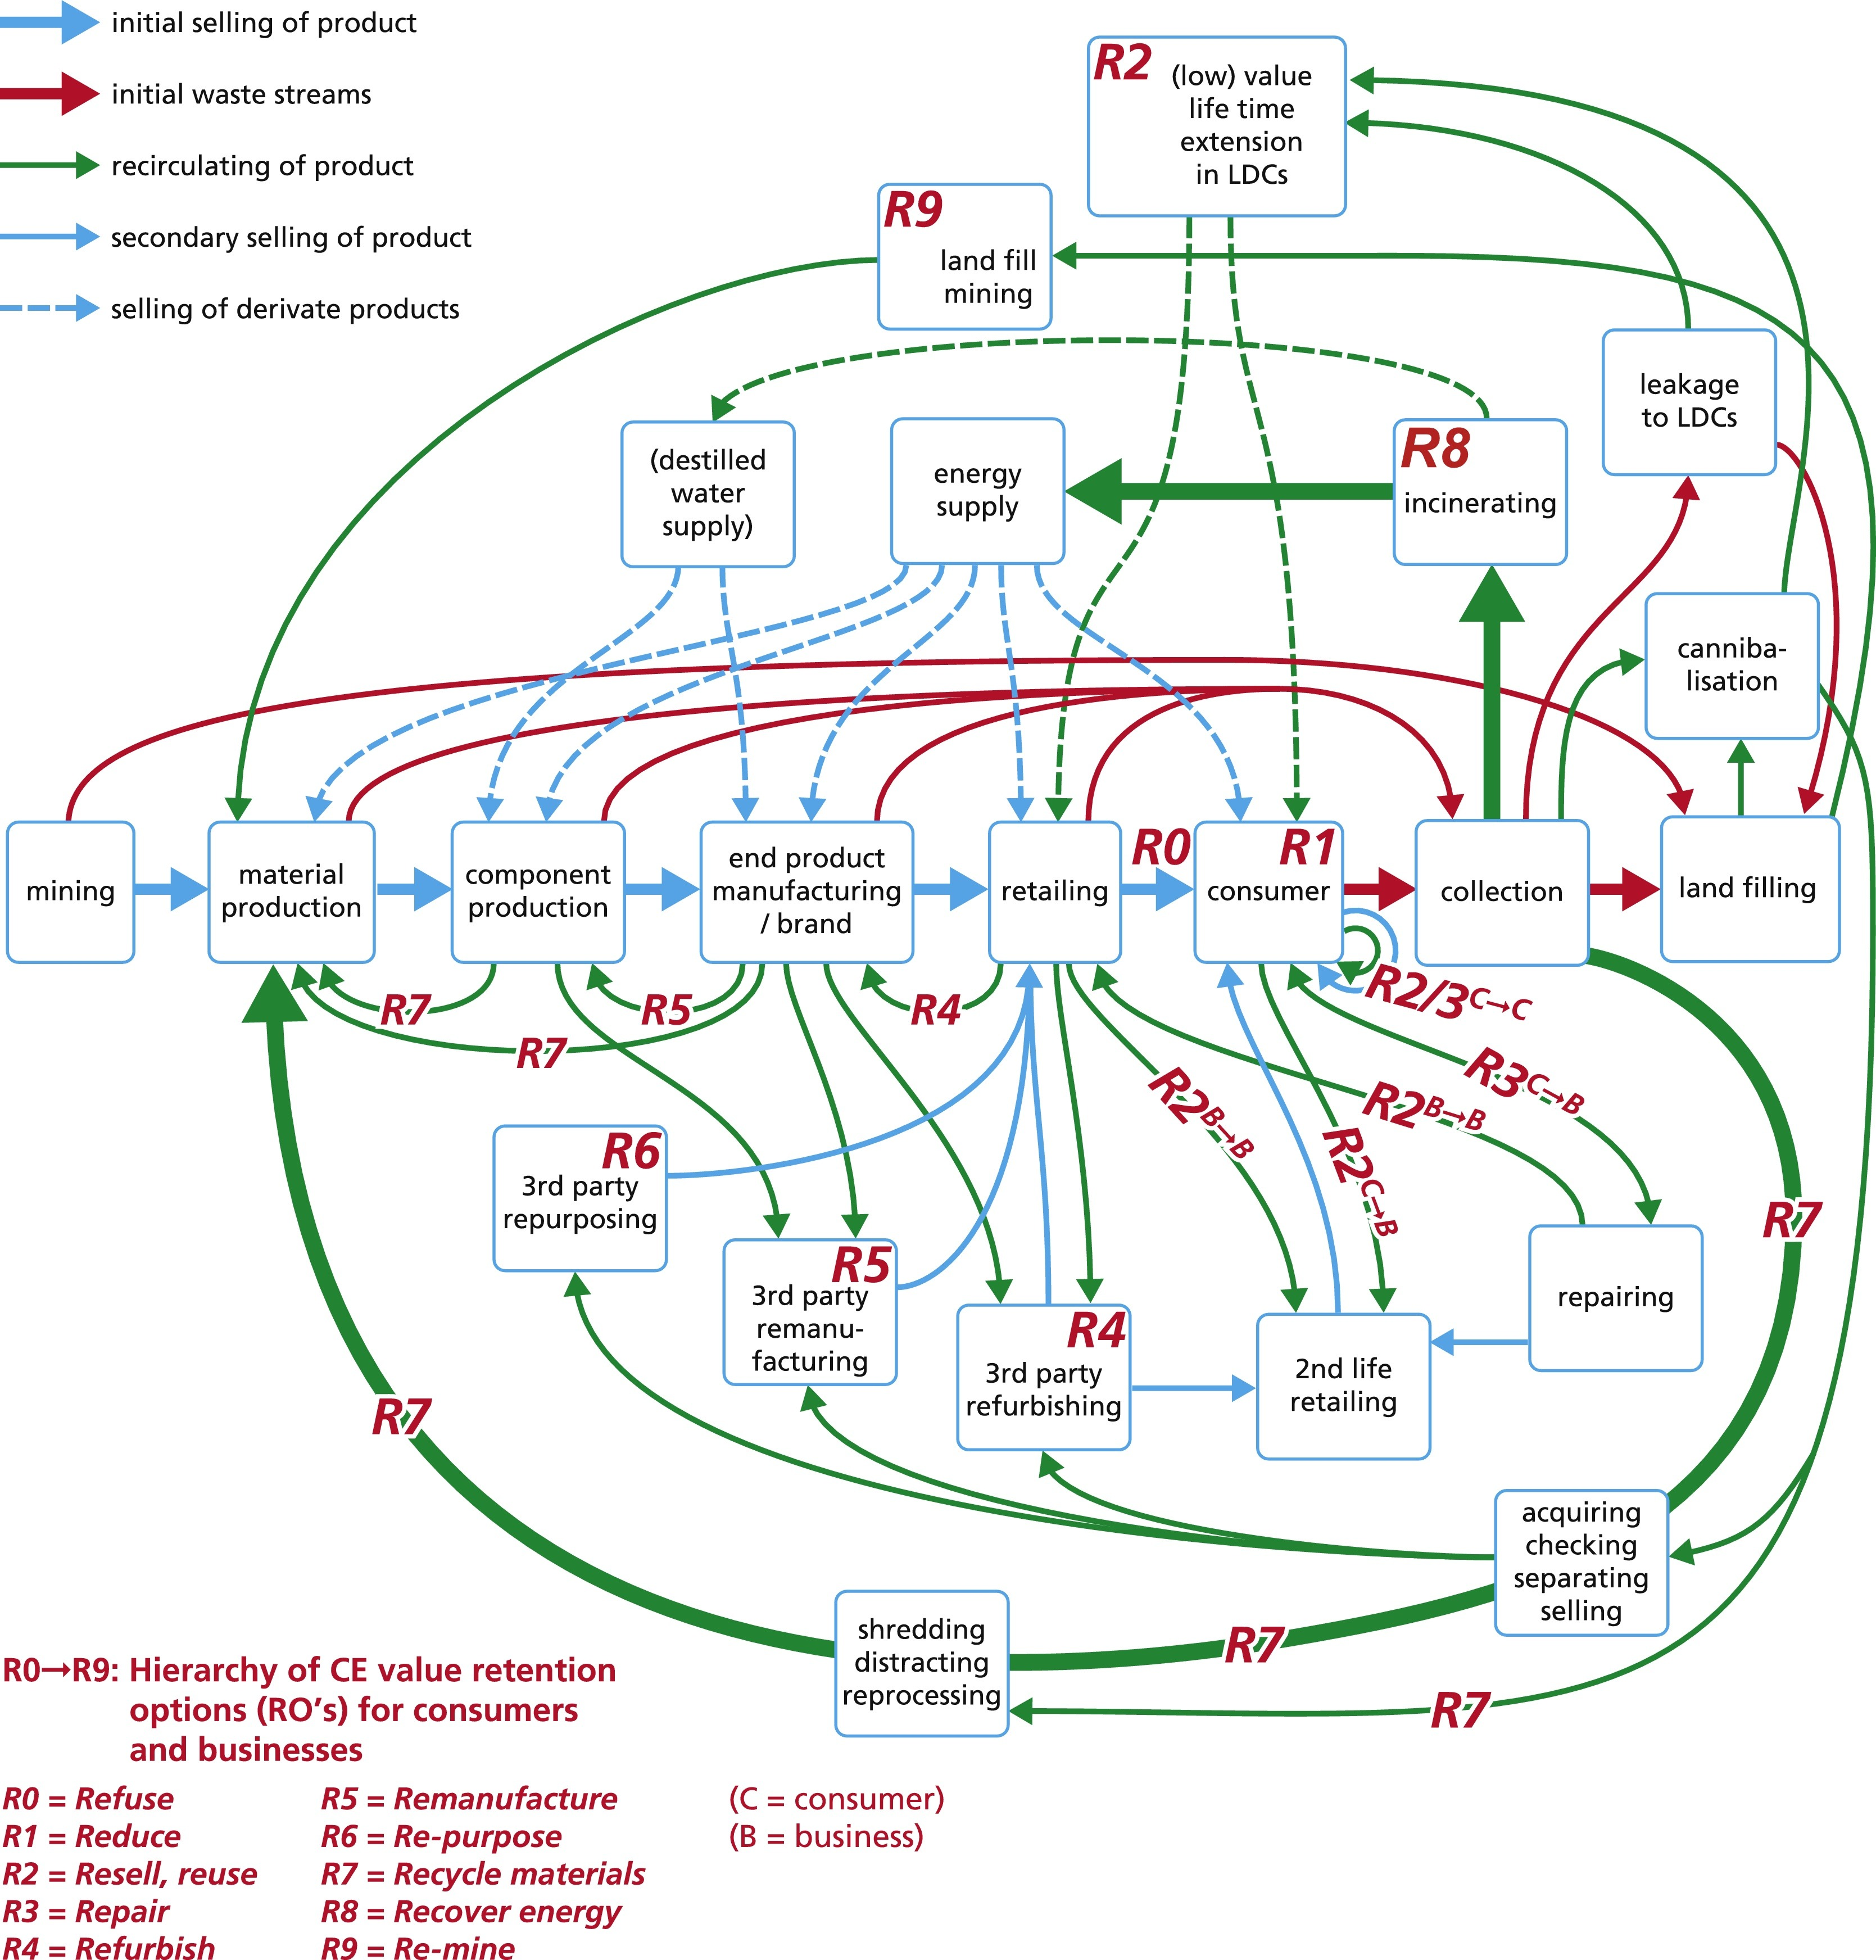
\includegraphics[width=\linewidth]{130quantification/internal/cei/reike2018.jpg}
    \caption[A detailled mapping of the re-X strategies in the circular economy]{A detailled mapping of the re-X strategies in the circular economy~\cite{reike2018rex}}
    \label{fig:rex-map}
\end{figure}
\FloatBarrier

\subsubsubsection{EU Circular Economy Indicators (CEIs)}

See the EU working documents~\cite{eu2018cemonitoring} and~\cite{eu2023cemonitoring} for more detailled assssment of progress relating to the CEIs. \autoref{tab:eu2023ceprogress} presents an overview of the EU's CEIs including their target for 2023.

\begin{table}[h!]
  \centering
  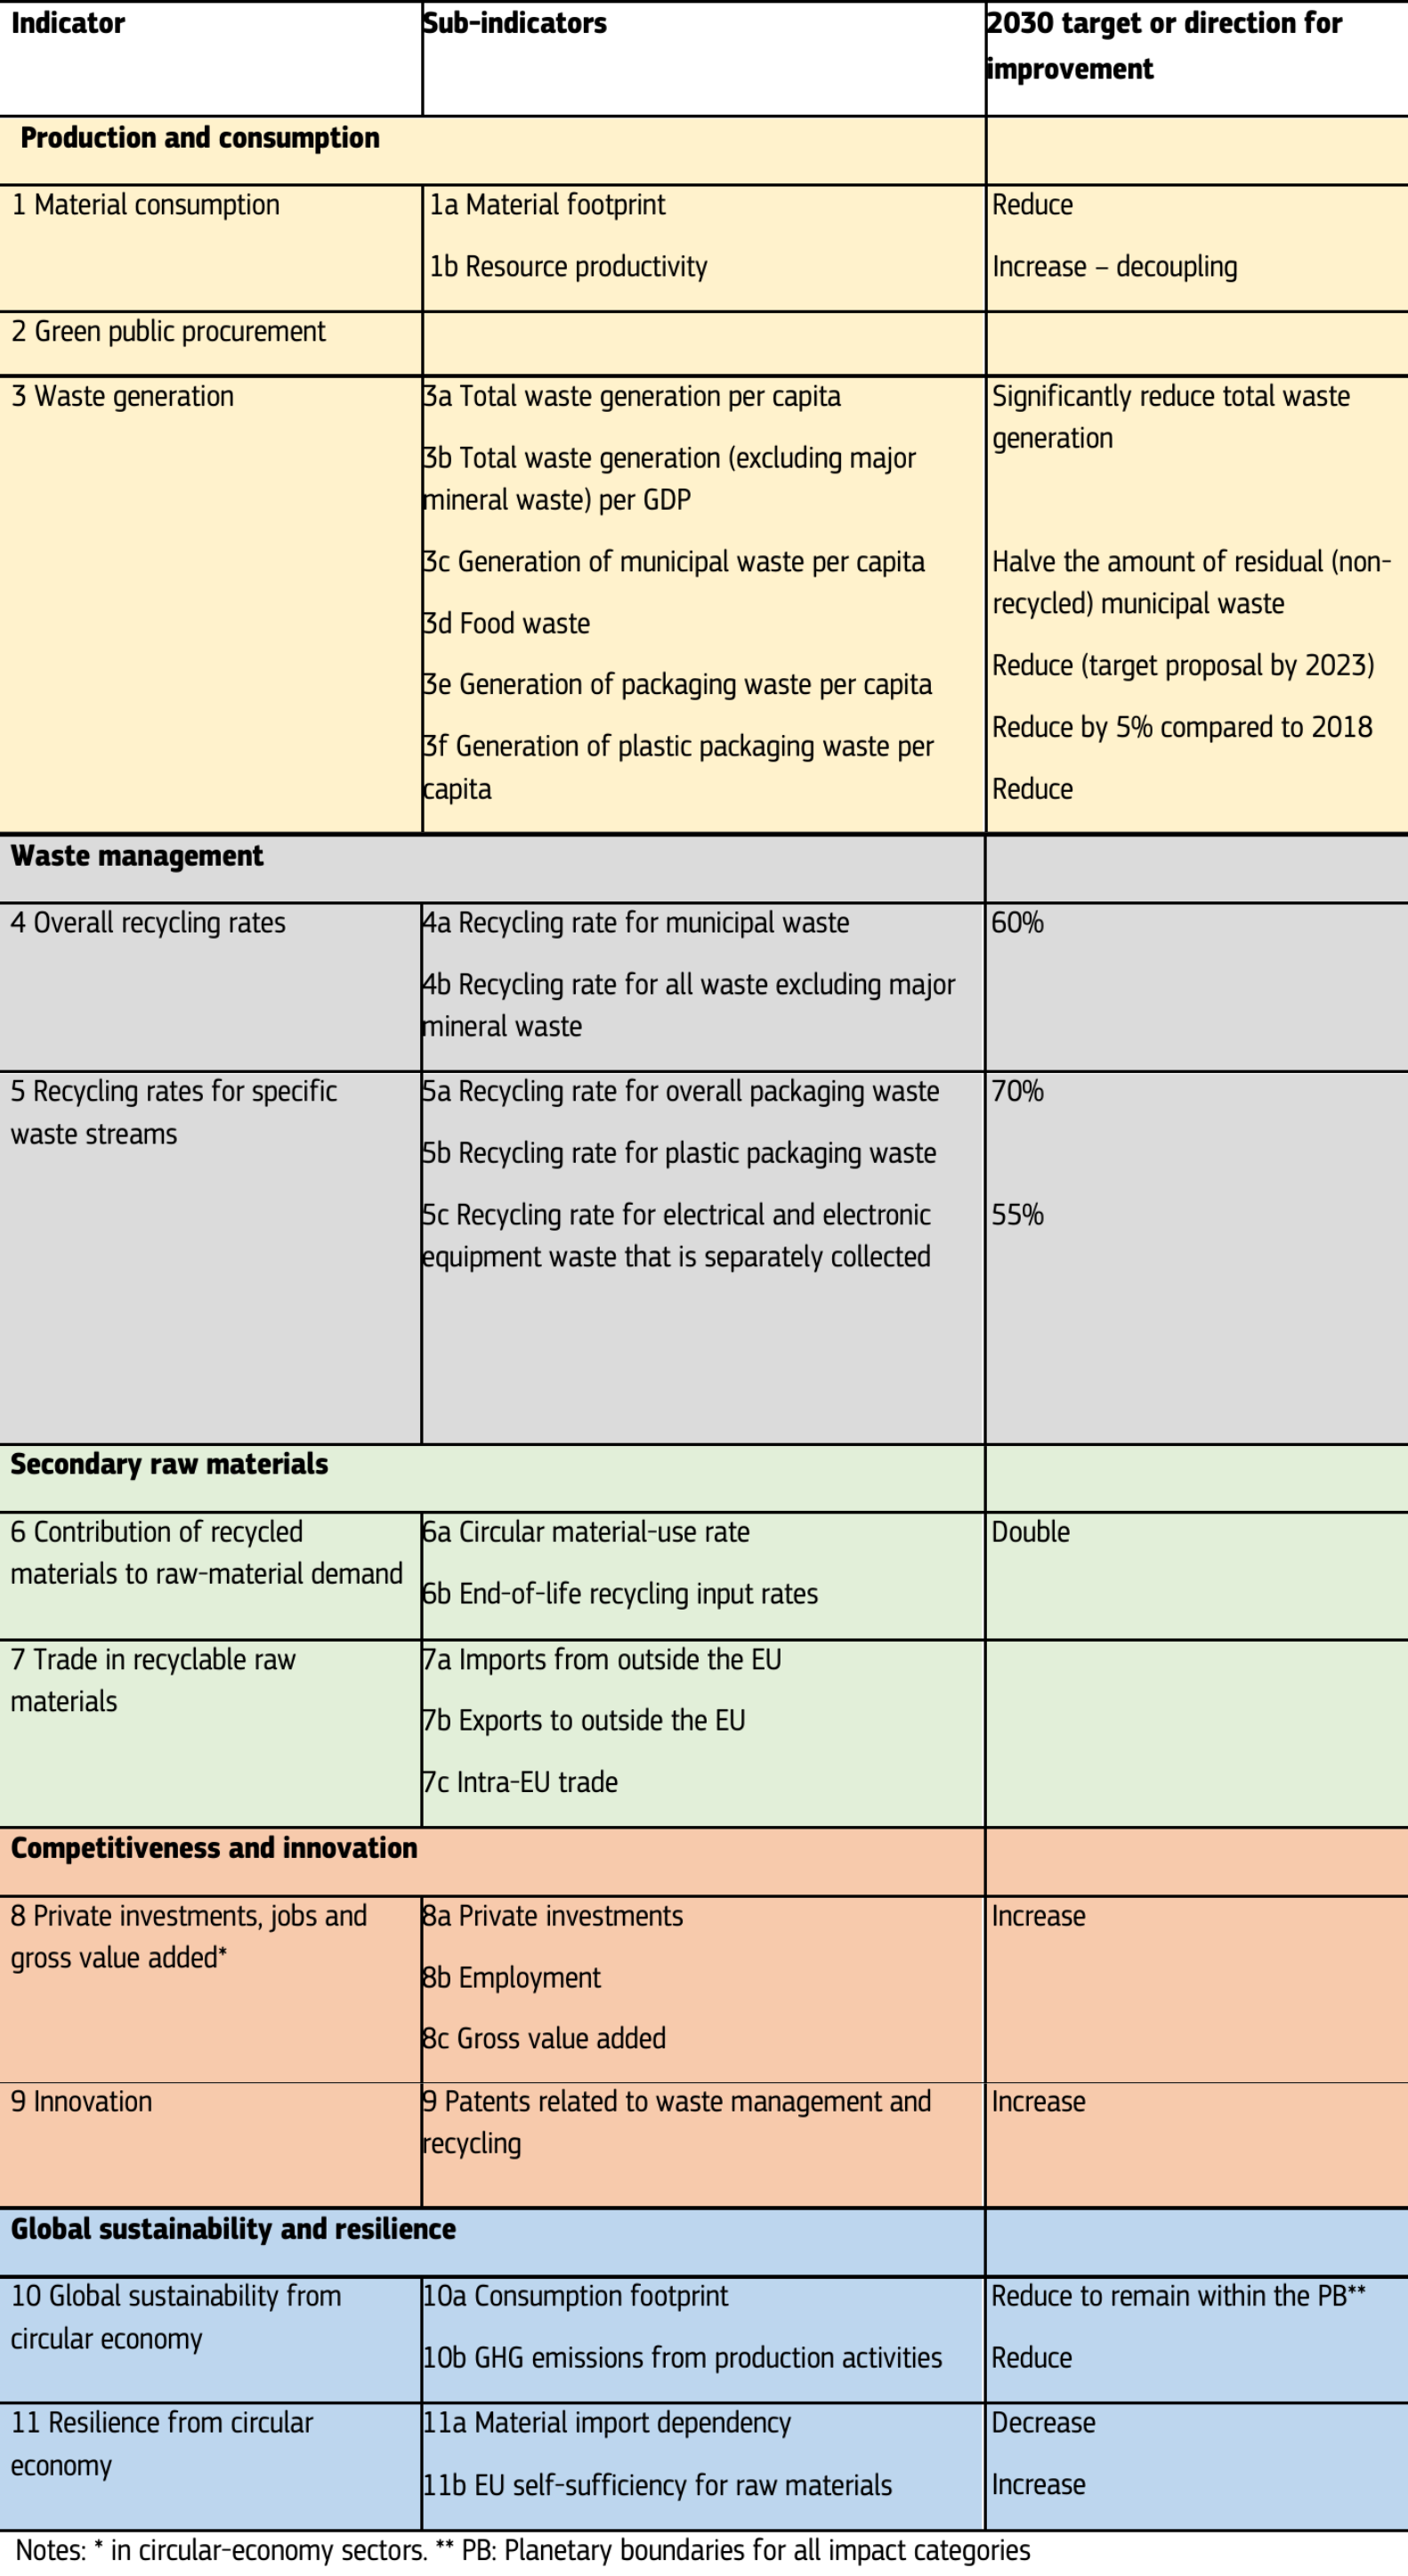
\includegraphics[height=0.9\textheight]{130quantification/internal/cei/eu2023ceprogress.png}
  \caption[EU Circular Economy Indicators (CEIs) and their targets for 2023]{EU Circular Economy Indicators (CEIs) and their targets for 2023~\cite{eu2023cemonitoring}}
  \label{tab:eu2023ceprogress}
\end{table}

\autoref{tab:cei} lists the relevant EU circular indicators (CEIs) along with their significance for FutuRaM's models and their changes between 2000--2022.

\begin{landscape}
    \centering
    \small
    \begin{longtable}{|C{2.5cm}|L{7cm}|C{6cm}|C{6cm}|C{1.5cm}|}
    \caption{EU circular indicators (CEIs) and their significance for FutuRaM's models}\label{tab:cei}\\
          \hline
          \rowcolor{headerblue} % Applying the header color
          \textcolor{white}{\textbf{CODE}} & \textcolor{white}{\textbf{TITLE}} & \textcolor{white}{\textbf{WS MODEL RELEVANCE}} & \textcolor{white}{\textbf{RECOVERY MODEL RELEVANCE}} & \textcolor{white}{\textbf{RATIO 2022:2000}} \\
          \hline
          \endfirsthead%
          \hline
          \multicolumn{5}{r}{\textcolor{headerblue}{\textit{{Continued on next page}}}} \\
          \endfoot%
          \rowcolor{white}
          \multicolumn{5}{c}{{\textcolor{headerblue}{\textit{\tablename\ \thetable{} --- Continued from previous page}}}} \\
          \hline
          \rowcolor{headerblue} % Applying the header color       
          \textcolor{white}{\textbf{CODE}} & \textcolor{white}{\textbf{TITLE}} & \textcolor{white}{\textbf{WS MODEL RELEVANCE}} & \textcolor{white}{\textbf{RECOVERY MODEL RELEVANCE}} & \textcolor{white}{\textbf{RATIO 2022:2000}} \\ \hline
          \endhead%
          \bottomrule
          \endlastfoot%
      \csvreader[late after last line=\ , separator=semicolon]{csvs/cei_eu.csv}{}{
        \csvcoli& \csvcolii& \csvcoliii& \csvcoliv& \csvcolv \\
      } \\
      \bottomrule
    \end{longtable}
  \end{landscape}


\autoref{fig:cei} depicts the CEIs, their trends from 2000-2022, and their linear forecasts until 2050. An interactive figure can be viewed \href{https://futuram-project.github.io/FutuRaM.github.io/WP2/assets.html}{here~\faLink}. Note that the linear trends are not deemed to be representative of the actual future values, but are used to illustrate the trends and the magnitude of the changes. There will be constraints defined to limit and shape the growth of the CEIs in each of the scenarios. The settings for this will be determined from the waste stream quantification and the scenario storylines.

\begin{landscape}
    \begin{figure}[h!]
        \centering
        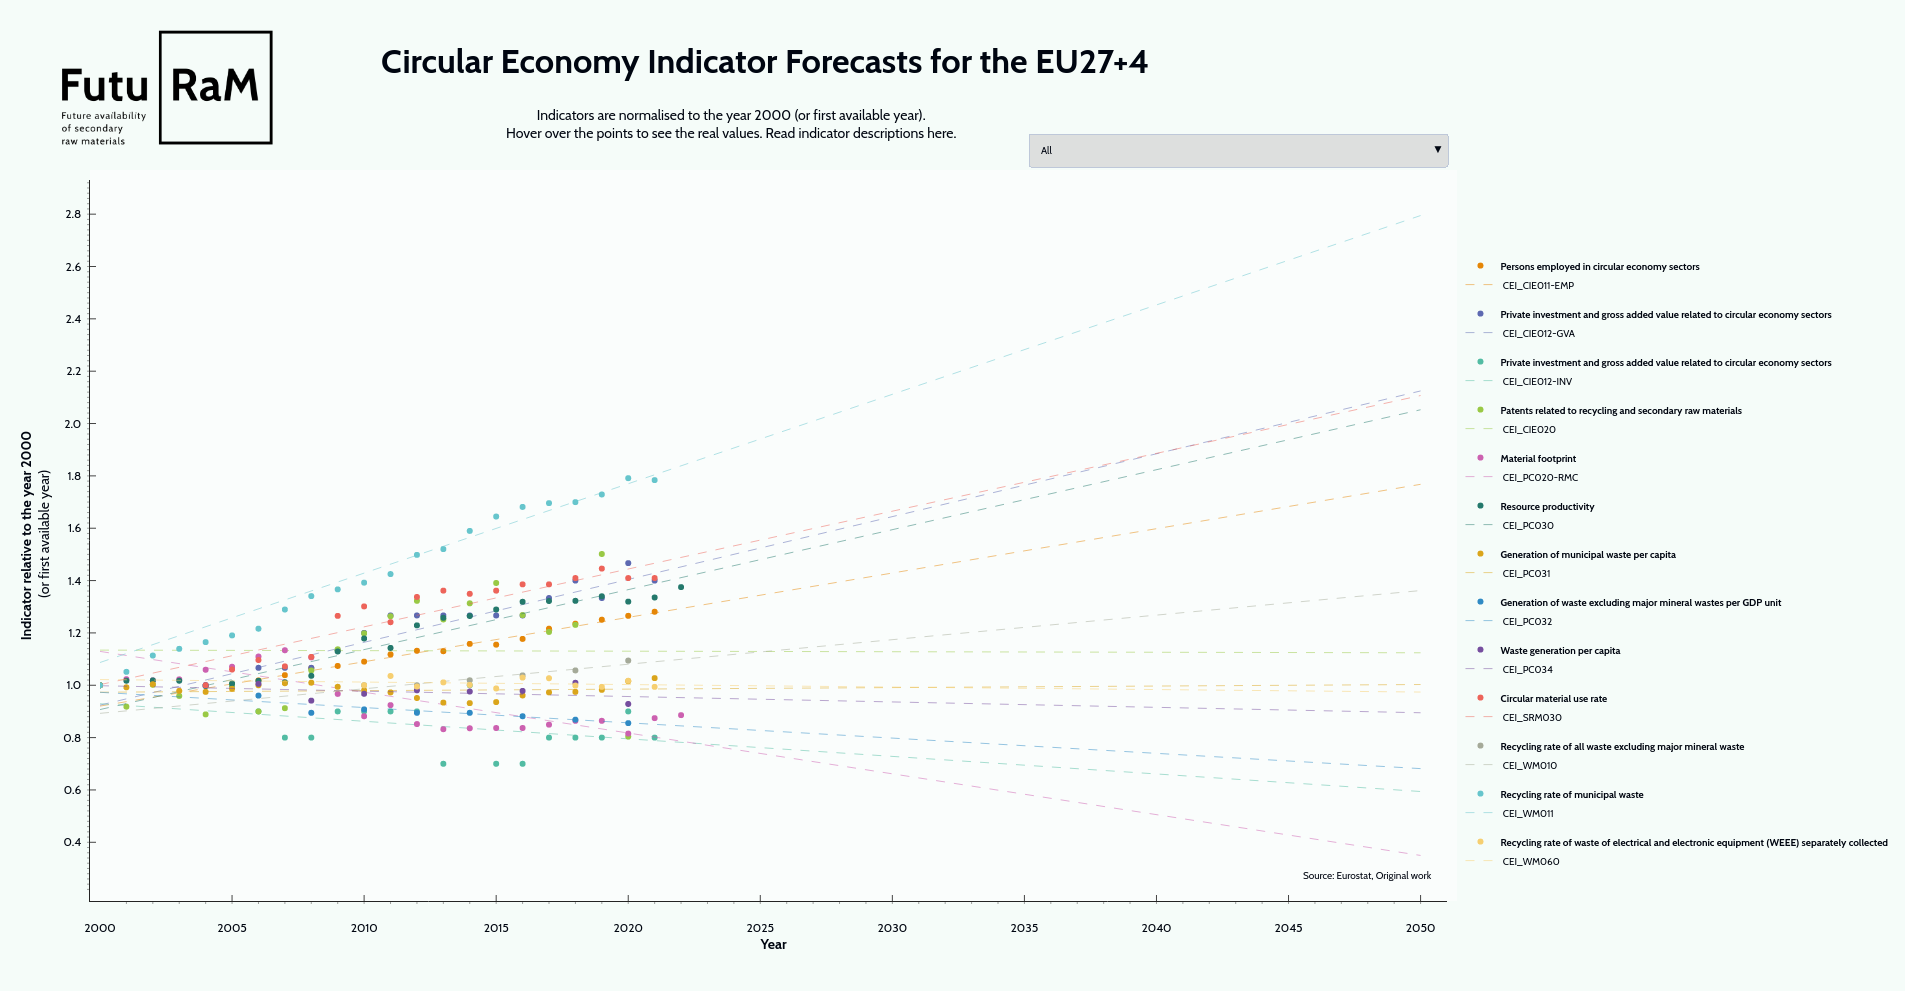
\includegraphics[width=1\linewidth]{130quantification/internal/cei/cei_eu.png}
        \caption{EU Circular Economy Indicators (CEIs) - trends from 2000-2022 and linear forecasts}
        \label{fig:cei}
    \end{figure}
\end{landscape}
    



\subsectionEndline
\clearpage

\subsection{Summary}


The environmental and socio-economic impacts of raw material use are most effectively addressed at the product group level. Examining a product group as a whole, rather than focusing on individual resources or materials, allows for a comprehensive understanding and management of its utilisation and the environmental impacts across the production chain and product lifecycle~\cite{pbl2021ce}. 

Additionally, setting impact targets for product groups aligns more closely with the capacity of stakeholders within the chain to modify resource usage or mitigate related environmental impacts.

Although the nature and magnitude of raw material use impacts can differ significantly among product groups, necessitating tailored impact targets, there is also a need for simplicity in target setting. A manageable and communicable approach for governments is to aim for a significant reduction, such as halving the environmental impact at the product group level. 

The benefit of establishing more general effect targets lies in the flexibility it offers for varying focuses across different product groups. A target set at the product group level is not only clear and easily communicable but also acknowledges the complexity and diversity inherent in a circular economy.


\boxreview{This section will be completed once the individual waste stream sections for each parameter are complete.}
\clearpage

% pull in the other subsections

\subsection{The EU Circular Economy Indicators: \textit{Description}}

\textbf{Main sources:}~\cite{eu2018cemonitoring,eurostat2023data,eu2023cemonitoring}


\boxparameter{The EU Circular Economy Indicators}{Stable}{Strong increase in recycling and recovery related indicators}{Strong in circularity related indicators}

\subsubsection{Economic Indicators}

\subsubsubsection{CEI\_CIE011:\\ Persons employed in circular economy sectors \& \\ CEI\_CIE012:\\ Private investment and gross added value related to circular economy sectors} 
\textbf{Indicator metadata:}   \href{https://ec.europa.eu/eurostat/cache/metadata/en/cei_cie011_esmsip2.htm}{\faExternalLink}

{\large\textbf{Context:}}  \\ \indent
Targets economic activities that contribute to the circular economy, delineating those activities through established environmental policy frameworks and classifications.

{\large\textbf{Indicator Description:}}  \\ \indent
The indicator encompasses ``Private investments'', ``Persons employed'' and ``Gross value added''. Eurostat has developed a method to derive these key economic variables, incorporating a multi-step approach: establishing a conceptual framework based on international environmental policy definitions, mapping and classifying relevant activities against an integrated system of economic classifications (using NACE, CPA, and PRODCOM codes), and finally compiling data using defined estimation procedures. The primary outputs of this process are the measurements of employment in FTE, gross value added at factor cost, and investments in tangible goods, each quantified in million euros.

{\large\textbf{Unit:}}  \\ \indent
Economic metrics are presented in million euros, with employment figures given in full-time equivalents (FTE); both sets of figures are also contextualised as percentages of GDP and total employment, respectively.

{\large\textbf{Source Data:}}  \\ \indent
Data is sourced from a combination of Structural Business Statistics, National Accounts, Prodcom surveys, and the Labour Force Survey, enriched by additional sector-specific statistics.

\subsubsubsection{CEI\_CIE020: Patents related to recycling and secondary raw materials}
\textbf{Indicator metadata:}   \href{https://ec.europa.eu/eurostat/cache/metadata/en/cei_cie020_esmsip2.htm}{\faExternalLink}

{\large\textbf{Context:}}  \\ \indent
This indicator is integral to the Circular Economy set, focusing on `competitiveness and innovation' and serving to gauge progress towards a more circular economy.

{\large\textbf{Indicator Description:}}  \\ \indent
The indicator enumerates the number of patent families pertinent to recycling and secondary raw materials, leveraging the Cooperative Patent Classification to ensure unique counts.

{\large\textbf{Unit:}}  \\ \indent
The unit of measure is the number of patent families, with a secondary metric of patents per million inhabitants.

{\large\textbf{Source Data:}}  \\ \indent
Sourced from the European Patent Office (EPO), the data are extracted and analyzed by the Joint Research Centre (JRC), using the PATSTAT database.

\subsubsubsection{CEI\_PC030: Resource productivity}
\textbf{Indicator metadata:}   \href{https://ec.europa.eu/eurostat/cache/metadata/en/cei_pc030_esmsip2.htm}{\faExternalLink}

{\large\textbf{Context:}} \\
Embedded within the Circular Economy indicator suite, this metric tracks progress in `Production and consumption', emphasizing material use efficiency to gauge economic growth relative to resource use.

{\large\textbf{Indicator Description:}}  \\ \indent
Resource productivity is articulated as GDP over DMC, showcasing the efficiency of material utilization within an economy. This indicator assists in understanding the dynamics between economic performance and environmental pressure.

{\large\textbf{Unit:}}  \\ \indent
Measured in three distinct units: euro per kg in chain-linked volumes (2015), PPS per kg, and as an index (2000=100) for temporal and spatial comparisons.

{\large\textbf{Source Data:}}  \\ \indent
The European Statistical System (ESS) supplies the data, with Eurostat disseminating information on DMC and GDP, derived from the Material Flow Accounts and GDP and main components datasets, respectively.

\subsubsection{Waste and Material Indicators}

\subsubsubsection{CEI\_PC020: Material footprint}
\textbf{Indicator metadata:}   \href{https://ec.europa.eu/eurostat/cache/metadata/en/cei_pc020_esmsip2.htm}{\faExternalLink}

{\large\textbf{Context:}}  \\ \indent
The `Material footprint' indicator is a critical component of the Circular Economy monitoring framework, highlighting the `production and consumption' thematic area. It reflects the EU's impact on global resources, pertinent to the EU's consumption exceeding its production, especially concerning goods manufactured in Asia and consumed in Europe.

{\large\textbf{Indicator Description:}}  \\ \indent
This indicator assesses the global demand for material extraction driven by EU consumption and investment. The Material Footprint provides insight into the environmental burden shifted to other regions due to the EU`s consumption patterns. It is expressed through the Raw Material Consumption (RMC) metric, indicating the material extraction required for goods consumed within the EU.

{\large\textbf{Unit:}}  \\ \indent
The unit of measure is tonnes per capita.

{\large\textbf{Source Data:}}  \\ \indent
Data source: European Statistical System (ESS)
Data provider: Statistical Office of the European Union (Eurostat).
Material flow accounts in raw material equivalents -- modelling estimates (env\_ac\_rme).~\href{https://ec.europa.eu/eurostat/web/products-datasets/-/env_ac_rmefd}{\faExternalLink}
Material flow accounts in raw material equivalents by final uses of products - modelling estimates (env\_ac\_rmefd).~\href{https://ec.europa.eu/eurostat/web/products-datasets/-/env_ac_rmefd}{\faExternalLink}

\subsubsubsection{CEI\_PC031: Generation of municipal waste per capita}
\textbf{Indicator metadata:}   \href{https://ec.europa.eu/eurostat/cache/metadata/en/cei_pc031_esmsip2.htm}{\faExternalLink}

{\large\textbf{Context:}}  \\ \indent
The `Generation of municipal waste per capita' indicator is integral to the Circular Economy indicator set, falling under the `production and consumption' thematic area. It underscores efforts to sustain product and material value in the economy, minimize waste generation, and drive waste prevention strategies in alignment with the Waste Hierarchy.

{\large\textbf{Indicator Description:}}  \\ \indent
This indicator tracks municipal waste generated and managed by local authorities or entities appointed by them. It predominantly accounts for household waste, although it may include waste from commercial activities, offices, and public institutions, reflecting consumer behaviour and the impact of waste reduction measures.

{\large\textbf{Unit:}}  \\ \indent
The unit of measure is kilograms per capita, based on the annual average population.

{\large\textbf{Source Data:}}  \\ \indent
The data is provided by Eurostat, consistent with the high-quality standards of the European Statistical System (ESS), deriving from the Municipal waste by waste operations report, collected under the OECD/Eurostat Joint Questionnaire. Data submission is voluntary, known as a `gentlemen's agreement'.

\subsubsubsection{CEI\_PC032: \\Generation of waste excluding major mineral wastes per GDP unit}
\textbf{Indicator metadata:}   \href{https://ec.europa.eu/eurostat/cache/metadata/en/cei_pc032_esmsip2.htm}{\faExternalLink}

{\large\textbf{Context:}}  \\ \indent
The `Generation of municipal waste per capita' indicator is integral to the Circular Economy indicator set, falling under the `production and consumption' thematic area. It underscores efforts to sustain product and material value in the economy, minimize waste generation, and drive waste prevention strategies in alignment with the Waste Hierarchy.

{\large\textbf{Indicator Description:}}  \\ \indent
This indicator tracks municipal waste generated and managed by local authorities or entities appointed by them. It predominantly accounts for household waste, although it may include waste from commercial activities, offices, and public institutions, reflecting consumer behaviour and the impact of waste reduction measures.

{\large\textbf{Unit:}}  \\ \indent
The unit of measure is kilograms per capita, based on the annual average population.

{\large\textbf{Source Data:}}  \\ \indent
The data is provided by Eurostat, consistent with the high-quality standards of the European Statistical System (ESS), deriving from the Municipal waste by waste operations report, collected under the OECD/Eurostat Joint Questionnaire. Data submission is voluntary, known as a gentlemen's agreement.

\subsubsubsection{CEI\_PC034: Waste generation per capita}
\textbf{Indicator metadata:}   \href{https://ec.europa.eu/eurostat/cache/metadata/en/cei_pc034_esmsip2.htm}{\faExternalLink}

{\large\textbf{Context:}}  \\ \indent
The `Waste generation per capita' indicator is a key component of the Circular Economy monitoring framework, aimed at assessing the effectiveness of EU policies focused on waste reduction and resource efficiency within the `production and consumption' thematic area.

{\large\textbf{Indicator Description:}}  \\ \indent
This indicator reflects the total waste generation within a country, including major mineral wastes from all economic activities and households. It is an essential measure for evaluating the impact of waste prevention measures, allowing comparison of Member States' performance over time.

{\large\textbf{Unit:}}  \\ \indent
The unit of measure is kilogram per capita

{\large\textbf{Source Data:}}  \\ \indent
The data originates from the European Statistical System (ESS), specifically Eurostat, which collates information reported by countries under the Waste Statistics Regulation (EC) No 2150/2002.

\subsubsubsection{CEI\_SRM030: Circular material use rate}
\textbf{Indicator metadata:}   \href{https://ec.europa.eu/eurostat/cache/metadata/en/cei_srm030_esmsip2.htm}{\faExternalLink}

{\large\textbf{Context:}}  \\ \indent
As a core metric within the Circular Economy indicator set, the `Circular material use rate' is crucial for monitoring advancements in the utilization of `secondary raw materials'. It encapsulates the circular economy's goal to enhance material recycling, reduce waste, and curb the reliance on primary raw material extraction.

{\large\textbf{Indicator Description:}}  \\ \indent
This indicator assesses the proportion of recycled material re-entering the economy against the overall material consumption, serving as a benchmark for the `circularity rate'. It signifies the efficiency of resource use by contrasting the circular use of materials against the aggregate domestic material consumption (DMC), adjusted for waste trade.

{\large\textbf{Unit:}}  \\ \indent
The indicator is presented as a percentage, depicting the share of recycled material in total material usage, reflecting the level at which secondary materials replace primary resources.

{\large\textbf{Source Data:}}  \\ \indent
Data is sourced from the European Statistical System (ESS) and Eurostat, employing a trio of statistical resources: waste treatment statistics, material flow accounts, and international trade data.

\subsubsubsection{CEI\_WM010: Recycling rate of all waste excluding major mineral waste}
\textbf{Indicator metadata:}   \href{https://ec.europa.eu/eurostat/cache/metadata/en/cei_wm010_esmsip2.htm}{\faExternalLink}

{\large\textbf{Context:}}  \\ \indent
This indicator is pivotal for measuring advancements in `waste management`. It gauges the efficiency of resource use by monitoring the volume of materials recycled and reincorporated into the economy, thus encapsulating the essence of material conservation and loss reduction.

{\large\textbf{Indicator Description:}}  \\ \indent
The recycling rate is formulated by the proportion of waste recycled versus the total waste treated, excluding significant mineral waste, rendered in percentage terms. It encompasses both hazardous and non-hazardous waste across all sectors, including household and secondary waste from waste treatment processes, thereby providing a comprehensive snapshot of the national recycling efforts.

{\large\textbf{Unit:}}  \\ \indent
Expressed in percentage

{\large\textbf{Source Data:}}  \\ \indent
Eurostat, under the aegis of the ESS, supplies this data. It incorporates waste treatment information aligned with the Waste Statistics Regulation, fine-tuned with international trade data, to accurately reflect the recycling of domestically produced waste.

\subsubsubsection{CEI\_WM011: Recycling rate of municipal waste}
\textbf{Indicator metadata:}   \href{https://ec.europa.eu/eurostat/cache/metadata/en/cei_wm011_esmsip2.htm}{\faExternalLink}

{\large\textbf{Context:}}  \\ \indent
As an integral part of the Circular Economy indicators, this measure serves as a barometer for the progression towards a more circular economy, with a focus on `waste management`. It assesses the re-utilisation of consumer waste in the economy, capturing the complexities inherent in the diverse composition of municipal waste.

{\large\textbf{Indicator Description:}}  \\ \indent
This indicator quantifies the proportion of municipal waste that is recycled, relative to the total amount of municipal waste produced, presented as a percentage. The breadth of municipal waste includes household refuse and similar commercial and public waste, representing a snapshot of the waste management quality from a consumer perspective.

\textit{"In order to comply with the objectives of this Directive, and move to a European circular economy with a high level of resource efficiency, Member States shall take the necessary measures designed to achieve the following targets: (a) by 2020, the preparing for re-use and the recycling of waste materials such as at least paper, metal, plastic and glass from households and possibly from other origins as far as these waste streams are similar to waste from households, shall be increased to a minimum of overall 50 \% by weight;"} --- Article 11.2 of the Waste Framework Directive.~\cite{eu2008wastedirective}

{\large\textbf{Unit:}}  \\ \indent
The metric of evaluation is a percentage

{\large\textbf{Source Data:}}  \\ \indent
Data source: European Statistical System (ESS)
Data provider: Statistical Office of the European Union (Eurostat) based on data reported by the countries: Municipal waste by waste operations \href{http://ec.europa.eu/eurostat/web/products-datasets/-/env_wasmun}{\faExternalLink} collected via a subset of the OECD/Eurostat Joint Questionnaire, section waste. Data are provided under a so-called gentlemen's agreement.

\subsubsubsection{CEI\_WM060: Recycling rate of waste of electrical and electronic equipment (WEEE) separately collected}
\textbf{Indicator metadata:}   \href{https://ec.europa.eu/eurostat/cache/metadata/en/cei_wm060_esmsip2.htm}{\faExternalLink}

{\large\textbf{Context:}}  \\ \indent
This indicator is a crucial component of the Circular Economy suite, offering insights into the progression towards enhanced sustainability in `waste management'. WEEE, or e-waste, is a rapidly expanding waste stream within the EU that encapsulates items like computers, TVs, refrigerators, and mobile phones. Given the valuable materials found in e-waste, improving recycling processes is of paramount importance.

{\large\textbf{Indicator Description:}}  \\ \indent
The indicator measures the efficiency of WEEE recycling by calculating the ratio of the weight of WEEE processed for recycling/re-use against the total weight of WEEE collected separately, in compliance with Article 11(2) of the WEEE Directive 2012/19/EU~\cite{eu2012weee, eu2012weeerecast}. The indicator's transition from `Recycling rate of e-waste' to its current form is to align more closely with the CE monitoring framework revisions.

The applicability of Directive 2012/19/EU is twofold:
\begin{itemize}
  \item Applicable up to the year 2018 for EEE classified under 10 product categories
        as outlined in Annex I of the Directive, with Annex II providing a
        corresponding indicative product list.
  \item Applicable from the year 2019 forward, where all EEE will be classified within
        6 product categories as delineated in Annex III.
\end{itemize}

{\large\textbf{Unit:}}  \\ \indent
The percentage serves as the unit of measure

{\large\textbf{Source Data:}}  \\ \indent \indent
Data procurement is executed by the ESS and supplied by Eurostat. The indicator's underlying data stems from:
\begin{itemize}
  \item For WEEE by waste operations:
        (env\_waselee)~\href{http://ec.europa.eu/eurostat/web/products-datasets/-/env_waselee}{\faExternalLink}.
  \item For WEEE by waste management operations - open scope, 6 product categories
        (from 2018 onwards):
        (env\_waseleeos)~\href{https://ec.europa.eu/eurostat/web/products-datasets/-/env_waseleeos}{\faExternalLink}.
\end{itemize}


\sectionEndlines
\clearpage

\clearpage
\subsection{The EU Circular Economy Indicators: \textit{Scenarios}}\label{subsec:cei-scenarios}

\boxws{This section will be filled out with the details of exactly how this parameter is incorporated into your stock and flow models}

\subsubsection{Summary}

\boxreview{This summary will be compiled once the individual waste stream sections for each parameter are complete.}

\clearpage

\subsubsection[Scenario I: Business-as-usual]{\iconBAU Scenario I: Business-as-usual}

xx \\


\wasteSubsubsubsecBATT

\wasteSubsubsubsecCDW

\wasteSubsubsubsecELV

\wasteSubsubsubsecMIN

\wasteSubsubsubsecSLASH

\wasteSubsubsubsecWEEE

\subsectionEndline
\clearpage

\subsubsection[Scenario II: Recovery]{\iconREC Scenario II: Recovery}

xx \\


\wasteSubsubsubsecBATT

\wasteSubsubsubsecCDW

\wasteSubsubsubsecELV

\wasteSubsubsubsecMIN

\wasteSubsubsubsecSLASH

\wasteSubsubsubsecWEEE

\subsectionEndline
\clearpage


\subsubsection[Scenario III: Circularity]{\iconCIR Scenario III: Circularity}

xx \\


\wasteSubsubsubsecBATT

\wasteSubsubsubsecCDW

\wasteSubsubsubsecELV

\wasteSubsubsubsecMIN

\wasteSubsubsubsecSLASH

\wasteSubsubsubsecWEEE

\sectionEndlines
\clearpage
\clearpage

\subsection{Refuse, Reduce, Reuse: \textit{Description}}

Refuse, Reduce, and Reuse are the first three short loops (R0-2) in the circular economy scheme. They exist close to the 
consumer and can be linked to commercial or non-commercial actors engaged in extending the product's lifespan~\cite{vermeulen2019rex}.

\boxparameter{Refuse, reduce, reuse}{Stable}{Stable}{Strong increase}


These strategies are pivotal in the circular economy, effectively reducing the environmental impact of products or services.

\begin{itemize}
    \item \textbf{R0 --- Refuse:} Choosing not to purchase products or services that are unnecessary or unsustainable. 
    \item \textbf{R1 --- Reduce:} Decreasing the quantity of products or services used or needed.
    \item \textbf{R2 --- Reuse:} Utilising products or services again for the same or a different purpose.
\end{itemize}

These strategies will be incorporated into FutuRaM's modelling framework through:

\begin{itemize}
    \item Waste volume reduction from:
    \begin{itemize}
        \item Reduction in overall demand, that is, the put on market (POM) of a product or service.
        \item Reduction in the amount of material used in a product or service (efficiency).
        \item Extension of the lifetime of products from reuse.
    \end{itemize}
    \item Changes in the composition of waste, as some products are more amenable to being refused or reused than others. 
\end{itemize}

\subsubsection{Definitions}

\subsubsubsection{Refuse}
Refuse encompasses consumer and producer decisions aimed at minimising waste creation and reducing environmental impact. For consumers, it involves choosing not to purchase products that are not environmentally friendly and reducing overall consumption. In the production context, it signifies the deliberate avoidance of certain materials or processes to enhance circularity, such as eschewing hazardous substances or designing to minimise waste. Refuse, as a concept, prioritises waste prevention at the source and is integral to fostering a more circular economy~\cite{reike2018rex}.

\subsubsubsection{Reduce}
Reduce refers to strategies aimed at minimising the use of natural resources, including energy, raw materials, and thereby reducing waste generation. This concept is multifaceted:

\begin{itemize}
    \item For consumers, it involves using products less frequently, caring for and repairing products to extend their life, and participating in the sharing economy.
    \item For producers, it focuses on using less material per production unit, often referred to as 'dematerialisation', and incorporating these principles early in the Concept and Design Life Cycle.
\end{itemize}

Reduction is also linked to the notion of Reuse, as decreasing the quantity of products (like cars) can incentivise their reuse. Policy measures to enforce reduction, such as banning single-use plastics or imposing environmental taxes, are essential for effective implementation~\cite{maitreekern2019rex}.

\subsubsubsection{Reuse}
Reuse is about extending the life of products in their original form for as long as possible, thus conserving resources and energy. It involves maintaining and repairing products to keep them in use and developing business models that support these practices. Examples include:

\begin{itemize}
    \item Reusable packaging initiatives in various industries.
    \item Encouraging the reuse of items like clothing, furniture, and electronics.
    \item Deposit-refund systems that incentivise product return and reuse.
\end{itemize}

Reuse strategies are vital for reducing the consumption of new products and avoiding the dichotomy of 'new for the rich, reused for the poor', promoting equitable and sustainable consumption patterns~\cite{morseletto2020cetargets}.



% \subsubsection{International and European Trends}

% \subsubsection{Implementation in EU Law}


% \subsubsection{Development of a metric for XXX}

% \subsubsection{Benefits and risks}

% \subsubsubsection{Environmental Benefits and Risks}

% \subsubsubsection{Manufacturers' Perspective}


% \subsubsubsection{Broader Economic and Environmental Implications}


% \subsubsection{Relevance of refuse, reduce and reuse to Critical Raw Materials in Waste Streams}

% The integration of the the re-X stragegies of refuse, reduce and reuse has implications for the management of Critical Raw Materials
% (CRMs) across various waste streams, such as BATT (waste batteries), ELV
% (end-of-life vehicles), WEEE (waste electrical and electronic equipment), and
% CDW (construction and demolition waste).

% \wasteSubsubsecBATT
% \begin{itemize}
%     \item
% \end{itemize}

% \wasteSubsubsecELV
% \begin{itemize}
%     \item
% \end{itemize}

% \wasteSubsubsecWEEE
% \begin{itemize}
%     \item
% \end{itemize}

% \wasteSubsubsecCDW
% \begin{itemize}
%     \item
% \end{itemize}

% \wasteSubsubsecMIN
% \begin{itemize}
%     \item
% \end{itemize}

% \wasteSubsubsecSLASH
% \begin{itemize}
%     \item
% \end{itemize}
\sectionEndlines
\clearpage

\clearpage
\subsection{Refuse, Reduce, Reuse: \textit{Scenarios}}\label{subsec:refuse-reduce-reuse-scenarios}

\boxws{This section will be filled out with the details of exactly how this parameter is incorporated into your stock and flow models}

\subsubsection{Summary}

\boxreview{This summary will be compiled once the individual waste stream sections for each parameter are complete.}

\clearpage

\subsubsection[Scenario I: Business-as-usual]{\iconBAU Scenario I: Business-as-usual}

xx \\


\wasteSubsubsubsecBATT

\wasteSubsubsubsecCDW

\wasteSubsubsubsecELV

\wasteSubsubsubsecMIN

\wasteSubsubsubsecSLASH

\wasteSubsubsubsecWEEE

\subsectionEndline
\clearpage

\subsubsection[Scenario II: Recovery]{\iconREC Scenario II: Recovery}

xx \\


\wasteSubsubsubsecBATT

\wasteSubsubsubsecCDW

\wasteSubsubsubsecELV

\wasteSubsubsubsecMIN

\wasteSubsubsubsecSLASH

\wasteSubsubsubsecWEEE

\subsectionEndline
\clearpage


\subsubsection[Scenario III: Circularity]{\iconCIR Scenario III: Circularity}

xx \\


\wasteSubsubsubsecBATT

\wasteSubsubsubsecCDW

\wasteSubsubsubsecELV

\wasteSubsubsubsecMIN

\wasteSubsubsubsecSLASH

\wasteSubsubsubsecWEEE

\sectionEndlines
\clearpage
\clearpage

\subsection{Repair: \textit{Description}}~\cite{cordella2021repairlca, wieser2018,svensson2018repair, hernandez2020repair, eu2019repair}

\subsubsection{Definition}
Right to repair refers to the concept that end users, business users as well as
consumers, of (generally) technical, electronic or automotive devices should be
allowed to freely repair these products. Four requirements are of particular
importance:

\begin{itemize}
    \item The device should be constructed and designed in a manner that allows repairs
          to be made easily;
    \item End users and independent repair providers should be able to access the original
          spare parts and necessary tools (software as well as physical tools) at fair
          market conditions;
    \item Repairs should, by design, be possible and not be hindered by software
          programming; and
    \item The repairability of a device should be clearly communicated by the
          manufacturer.
\end{itemize}


\boxparameter{Repair}{Stable}{Stable}{Strong increase}


\subsubsection{Context}

Discarded products are often viable goods that can be repaired but are often
tossed prematurely, resulting in 35 million tons of waste, 30 million tons of
resources and 261 million tons of greenhouse gas emissions in the EU every
year~\cite{moeslinger2022repair}

Repairing is one of the most relevant strategies within the Circular Economy
(CE) concept since it contributes to waste prevention and extends product and
components' lifespan. Thus, reparability becomes an essential issue from the
early product design phases, where materials, geometries, and joints are
defined. Despite some repairability indicators that can be found in the
literature and are applied worldwide, there is a lack of connection between
repairability and the early decision-making process for improving it from the
design of components or subsystems of a product.

However, repair is often seen as difficult by consumers. The `right to repair'
initiative complements several other proposals presented by the Commission to
achieve sustainable consumption throughout the entire lifecycle of a product,
setting the framework for a true `right to repair' across the EU. Obstacles to
owner repair can lead to higher consumer costs or drive consumers to single-use
devices instead of making repairs.

The right to repair is a legal right for owners of devices and equipment to
freely modify and repair products such as automobiles, electronics, and farm
equipment. This right is framed in opposition to restrictions such as
requirements to use only the manufacturer's maintenance services, restrictions
on access to tools and components, and software barriers.

A right to repair can exist either in a closed access system, where the
consumer is restricted to the repair services provided by the manufacturer or
authorized repairers --- a situation closer to the current reality. Or, a right
to repair can evolve in an open access system, which implies full access to
spare parts, tools, repair manuals and digital permission to repair. Policy
options for a right to repair differ based on whether they encourage one or the
other approach. Some argue an open access system is the only form of right to
repair that is consumer-empowering and can yield the expected benefits. Others
argue for a more complex system, moving towards open access but with some
safeguards on a sectoral or product category basis. A cost-benefit analysis
could help identify the sectors or product categories where a full open-access
system would be most beneficial.

The goals of the right to repair are to favour repair instead of replacement and
make such repairs more affordable leading to a more sustainable economy and
reduction in waste.

\subsubsection{International and European Right to Repair Initiatives}~\cite{svensson2018repair, hernandez2020repair, eu2019repair}
\begin{itemize}
    \item \textbf{Availability of Spare Parts and Repair Information:}
          \begin{itemize}
              \item US state-level legislation includes laws like Massachusetts' requirement for
                    car manufacturers to provide repair tools and information.
              \item The EU has measures like France's mandate for sellers to inform about the
                    availability of spare parts, and Slovenia's requirement for maintenance and
                    spare parts for at least 3 years after guarantee expiration.
          \end{itemize}

    \item \textbf{Legal Guarantees:}
          \begin{itemize}
              \item European legal guarantee periods often exceed the EU directive's minimum,
                    encouraging repair culture.
              \item For example, Sweden has a 3-year guarantee period, and Finland ties the period
                    to the expected lifespan of the product.
          \end{itemize}

    \item \textbf{Design Requirements:}
          \begin{itemize}
              \item Legislation like Washington State's (USA) proposed fair repair bill is aimed
                    at promoting repairable product designs by prohibiting the creation of
                    electronics that obstruct repairability.
          \end{itemize}

    \item \textbf{Financial Incentives:}
          \begin{itemize}
              \item Cities like Graz offer subsidies for electronic device repairs and countries
                    like Belgium provide écochèques to incentivize repair over replacement.
          \end{itemize}

    \item \textbf{Copyright Law Exemptions:}
          \begin{itemize}
              \item In the US, certain copyright law exemptions facilitate repairability, such as
                    the ability to unlock phones, although the exemption renewal process is
                    cumbersome.
          \end{itemize}

    \item \textbf{Consumer Information:}
          \begin{itemize}
              \item France's reparability index helps inform consumers by rating products on
                    repairability criteria, promoting repair-friendly designs.
          \end{itemize}

    \item \textbf{Voluntary Labels and Green Public Procurement:}
          \begin{itemize}
              \item Ecolabels such as EPEAT and various national labels incorporate repairability
                    to different degrees.
              \item Green Public Procurement practices push the market towards sustainable,
                    repairable products.
          \end{itemize}

    \item \textbf{Communication and Awareness:}
          \begin{itemize}
              \item Initiatives include repair-focused websites, awareness campaigns, and the
                    establishment of repair hubs to build a repair-oriented culture.
          \end{itemize}
\end{itemize}

\subsubsection{Implementation in EU Law}~\cite{eu2023repair, moeslinger2022repair}

European Product Policy has to date focused on the environmental performance of
products via the Ecodesign and Ecolabelling Directives. The Ecodesign Directive
sets minimum standards of performance for products, which results in poorly
performing products being removed from the market whilst also driving
innovation in the design and manufacture of new products to improve their
performance. The Ecolabelling Directive provides consumers with clear
information on product performance to inform their buying decisions. Originally
cast for energy-using products, the directives have been extended to
energy-related products and the assessment methodologies have been developed to
include other aspects including materials and water consumption.

Further measures considered include:

\begin{itemize}
    \item Amending Directive 2005/29/EC to prohibit presenting products as allowing
          repair when such repair is not possible, as well as omitting to inform
          consumers that it is not possible to repair goods in accordance with legal
          requirements.
    \item Amending Directive 2005/29/EC to prohibit omitting to inform the consumer that
          the good is designed to limit its functionality when using consumables, spare
          parts, or accessories that are not provided by the original producer.
    \item Traders to provide, before the conclusion of the contract, for all types of
          goods, where applicable, the reparability score of the good as provided by the
          producer in accordance with Union law, to allow consumers to make an informed
          transactional decision and choose goods that are easier to repair.
    \item Ensuring information such as on the availability of spare parts and a repair
          manual, should no reparability score be available at the Union level.
\end{itemize}

To this end, new ‘Digital Product Passports’ providing information about
products’ environmental sustainability, will empower consumers and businesses
to make informed choices when purchasing products, facilitate repairs and
recycling, and improve transparency about products’ lifecycle impacts on the
environment. The passports also help public authorities to better perform
checks and controls.

In addition, as part of the implementation of the EU Circular Economy Action
Plan~\cite{eu2020circ}, the European Commission has carried out a study for the
analysis and development of a possible scoring system to inform about the
ability to repair and upgrade products~\cite{eu2019repair} and has an ongoing
project in the Product Bureau to develop and propose new
metrics~\cite{eu2023repairproject, eu2022repair}.

\subsubsection{Development of a metric for repairability}~\cite{eu2019repair, moeslinger2022repair, ruizpastor2023repair, eu2023repair, barros2023repair,eu2022repair, eu2023repairproject,sagar2022repair}

The trend in consumer goods towards reduced durability and repairability has
been contributing to an increase in waste electronic and electrical equipment
(WEEE). The Organization for Economic Co-operation and Development has
suggested that extending product lifetimes through enhanced durability and
repairability is a viable solution to this growing issue. The European
Commission's Circular Economy Action Plan reinforces this viewpoint, advocating
for maintaining the value in products for as long as possible by imposing
durability and repairability requirements. In response, several scoring systems
for repairability have been developed to guide standardization efforts, aid
market surveillance authorities, and inform consumer decision-making.

For a scoring system to be effective, it should provide an objective evaluation
of repairability that aligns with the established design principles in the
literature. Comparative analyses of various repairability scoring systems for
different products have been undertaken in previous studies. However, the
thoroughness of these systems is sometimes not fully evaluated, and some of the
most recent systems have not been comprehensively reviewed.

Literature on the subject identifies specific design features and principles
that significantly affect product repairability, and these should be central to
any scoring system aimed at accurately measuring repairability. Assessing these
design elements against selected scoring systems can shed light on their
inclusiveness.

The objectivity of these scoring systems is another critical aspect, evaluated
by examining their scoring methodologies. Selection criteria for these systems
include their availability in English, the use of quantitative or
semi-quantitative assessment methods to enable objective comparison, and their
recognition as the most current versions from their respective issuing
organizations or groups.

In 2021, France took a pioneering step by integrating the reparability index
into national legislation.~\cite{france2020repair} This move compels producers
to transparently communicate the repairability of their products through
consumer labelling. The reparability index stands as a key development in
empowering consumers to make informed choices regarding the repairability of
products. The widespread issue of repairing common electronic devices like
laptops and smartphones often stems from the unavailability of tools, spare
parts, or repair instructions.

An exemplary repair index would encompass elements such as product design, the
availability of repair information, and additional services like the
availability of spare parts. These aspects are crucial for the repair process.
Data indicates that a substantial number of electronic product repairs are
hindered by the lack of available spare parts.

France's method mandates transparency regarding product repairability, yet
relies on producers' self-assessment, prompting questions about the objectivity
of such evaluations. The rapid implementation is advantageous, but the
credibility of self-assessment remains a concern.

With sustainability becoming increasingly important, France's repairability
index marks an assertive step towards the broader adoption of such measures.
Looking ahead, enhancements like a durability index may offer greater insights
into the long-term usability of products.

In parallel, organizations such as TÜV SÜD are actively supporting the
repairability testing landscape, aligning with standards like the French
Repairability Scoring Index to ensure products fulfil specified repairability
criteria~\cite{tuv2023repair}. Their approach factors in documentation,
disassembly, and the availability of spare parts and repair services,
highlighting a practical, though less detailed, framework compared to France's
comprehensive index.

\subsubsection{Benefits and risks}

\subsubsubsection{Environmental Benefits and Risks}~\cite{eu2019repair, boulos2015durability, }

The implementation of the right to repair holds considerable promise for the
reduction of environmental impacts if applied appropriately. It must be
recognized that electronic equipment replacement often occurs not solely due to
product failure. Influencing factors such as perceived obsolescence contribute
significantly, as evidenced by a study in Austria revealing only 30\% of
replacements were attributable to malfunctioning products~\cite{wieser2018}.

Direct measurement of the impact of a right to repair is challenging, with the
need to consider additional variables such as obsolescence perception, device
performance, and consumer behaviour trends in determining potential extensions
in consumer electronics' average lifespan.

Moreover, the environmental benefit of repair is contingent not only on the
increased product lifespan post-repair but also on the environmental footprint
of the spare parts required for repair. Circuit boards, for example, carry
substantial environmental impacts, and their replacement could still result in
significant environmental costs. Common repairs typically involve less
impactful components such as screens, casings, batteries, or
software~\cite{cordella2021repairlca}.

Cordella et al.~\cite{cordella2021repairlca} report that compared to the
baseline of replacing smartphones every two years,
extending the device's life through repair can substantially diminish the
carbon footprint. A one-year extension, with a battery change, can reduce
greenhouse gas (GHG) emissions by 29\%, and by 44\% with a two-year extension.

With 472 million Europeans owning a mobile phone, there are \(8.11 \text{ Mt
    CO}_2\text{-eq.}\) in annual emissions solely from phones. Extending the life
of a mobile phone by just one year, including component replacements, could
reduce emissions to \(6.23 \text{ Mt CO}_2\text{-eq.}\)
annually~\cite{moeslinger2022repair}. A further extension by an additional year
could decrease emissions to \(4.91 \text{ Mt CO}_2\text{-eq.}\), effectively
removing the equivalent of over 2 million cars from European roads.

Nevertheless, these potential reductions should be interpreted with caution as
they are based on estimations and may not account for potential rebound
effects. For instance, economic savings from prolonged use of electronic
devices could lead to rebound effects where savings are offset by additional
consumption stemming from the economic savings~\cite{makov2018sharing}.

Finally, repair activities offer a more energy-efficient alternative within the
Circular Economy compared to recycling and remanufacturing, which demand
extensive energy input and high material throughput. When feasible, repair
should be prioritized over other circular economy
strategies~\cite{eu2019repair}.

\subsubsubsection{Manufacturers' Perspective}
\begin{itemize}
    \item Compliance with eco-design standards could reduce profit margins.
    \item Risk of increased liability and the need to ensure long-term availability of
          spare parts.
    \item Potential decrease in turnover due to extended product lifecycles.
    \item Reduction in EU imports could foster the EU's technological independence, as per
          the EU Chips Act.
    \item Loss in turnover potentially offset by repair services and spare parts supply.
\end{itemize}

\subsubsubsection{Broader Economic and Environmental Implications}
\begin{itemize}
    \item Right to Repair could enhance competitiveness by increasing product longevity
          and added value.
    \item Positive impact on professional repair services, spare parts provision, and
          tool providers.
    \item SMEs and local repair shops likely to benefit significantly.
    \item Potential for the development of new European leaders in repair services.
    \item A more repairable design could improve recycling processes and increase
          component harvesting.
\end{itemize}

\subsubsection{Relevance of Repairability to Critical Raw Materials in Waste Streams}

The integration of the `Right to Repair' ethos and the promotion of
repairability has implications for the management of Critical Raw Materials
(CRMs) across various waste streams, such as BATT (waste batteries), ELV
(end-of-life vehicles), WEEE (waste electrical and electronic equipment), and
CDW (construction and demolition waste).

\subsubsubsection{Batteries (BATT)}
Batteries are a crucial repository of CRMs like lithium, cobalt, and nickel. Enhancing their repairability can lead to:
\begin{itemize}
    \item Refurbishing batteries for second-life applications.
    \item Design modifications for easier replacement of battery cells.
    \item Reduced extraction of new raw materials, mitigating the environmental
          footprint.
\end{itemize}

\subsubsubsection{End-of-Life Vehicles (ELV)}
Vehicles are a significant source of CRMs such as platinum and palladium (catalytic converters) and rare earth elements (electronics and magnets). `Right to Repair' can:
\begin{itemize}
    \item Influence design changes for modularity and ease of part replacement.
    \item Prolong the utility of CRMs and lessen new resource extraction.
\end{itemize}

\subsubsubsection{Waste Electrical and Electronic Equipment (WEEE)}
The WEEE stream contains valuable CRMs like gold, silver, and rare earth elements. Promoting repairability results in:
\begin{itemize}
    \item Prolonged life spans for electronic devices.
    \item A reduction in the volume of CRMs entering the waste stream.
    \item Conservation of valuable materials through repair and refurbishment.
\end{itemize}

\subsubsubsection{Construction and Demolition Waste (CDW)}
CRMs feature in many building materials as well as wind turbines which are part of this waste stream, and advocating for repairability in construction can:
\begin{itemize}
    \item Lead to buildings designed for deconstruction, not demolition.
\end{itemize}

The emphasis on repairability and `Right to Repair' legislation can lead to
reduced CRM demand, decreased environmental impact through less mining,
creation of economic incentives for repair industries, and improved resource
security by minimizing reliance on raw material extraction. This approach is in
line with fostering a circular economy, aiming for a sustainable management of
resources within the EU.


\sectionEndlines
\clearpage
\clearpage
\subsection{Repair: \textit{Scenarios}}\label{subsec:repair-scenarios}

\boxws{This section will be filled out with the details of exactly how this parameter is incorporated into your stock and flow models}

\subsubsection{Summary}

\boxreview{This summary will be compiled once the individual waste stream sections for each parameter are complete.}

\clearpage

\subsubsection[Scenario I: Business-as-usual]{\iconBAU Scenario I: Business-as-usual}

xx \\


\wasteSubsubsubsecBATT

\wasteSubsubsubsecCDW

\wasteSubsubsubsecELV

\wasteSubsubsubsecMIN

\wasteSubsubsubsecSLASH

\wasteSubsubsubsecWEEE

\subsectionEndline
\clearpage

\subsubsection[Scenario II: Recovery]{\iconREC Scenario II: Recovery}

xx \\


\wasteSubsubsubsecBATT

\wasteSubsubsubsecCDW

\wasteSubsubsubsecELV

\wasteSubsubsubsecMIN

\wasteSubsubsubsecSLASH

\wasteSubsubsubsecWEEE

\subsectionEndline
\clearpage


\subsubsection[Scenario III: Circularity]{\iconCIR Scenario III: Circularity}

xx \\


\wasteSubsubsubsecBATT

\wasteSubsubsubsecCDW

\wasteSubsubsubsecELV

\wasteSubsubsubsecMIN

\wasteSubsubsubsecSLASH

\wasteSubsubsubsecWEEE

\sectionEndlines
\clearpage
\clearpage

\subsection{Remanufacturing and Refurbishing: \textit{Description}}

\subsubsection{Definition}
Remanufacturing involves disassembling the full structure of a multi-component product, inspecting, cleaning, repairing, or replacing necessary parts, and reassembling it to its original state or better. This process can include both reused and new components, aiming to achieve a quality level that meets or exceeds the new product~\cite{reike2018rex, sihvonena2015reman, zhang2012reman}.

Refurbishing, often confused with remanufacturing, is the process where the overall structure of a large multi-component product remains intact, while components are replaced or repaired, resulting in an overall ‘upgrade’ of the product. It aims to bring the product up to a specified quality, possibly incorporating newer, more advanced components~\cite{reike2018rex}.

\boxparameter{Remanufacturing and Refurbishing}{Stable}{Stable}{Strong increase}

\subsubsection{Context}
Remanufacturing and refurbishing are essential strategies in the circular economy, aimed at extending product lifecycles and reducing waste. They are particularly relevant in the medium loops (R4-R6) of product recovery, where they serve as business activities indirectly linked to the consumer~\cite{eu2015reman}.

\subsubsection{International and European Trends}
Remanufacturing is gaining momentum globally, particularly in the U.S. and Europe. Governments are legislating manufacturers to assume responsibility for their products post-use, emphasizing recyclability and waste reduction. The market for environmentally friendly products, valued at over USD 200 billion, is driving corporations to adopt remanufacturing and other green practices~\cite{mitra2005reman,irp2018manufacturing}.

\subsubsection{Implementation in EU Law}
EU laws increasingly mandate manufacturers to engage in product recovery, including remanufacturing. This aligns with the EU's broader goals of sustainable development, resource efficiency, and transitioning to a circular economy~\cite{eu2015reman,eu2019greendeal}.

\subsubsection{Economic Scale and Regional Focus in Europe}
The remanufacturing industry in Europe generates around €30bn in turnover and employs about 190,000 people. Key regions like Germany, the UK, Ireland, France, and Italy have significant remanufacturing activities. Germany leads in remanufacturing turnover, particularly in aerospace, automotive, and heavy-duty off-road (HDOR) sectors~\cite{eu2015reman}.

\subsubsection{Benefits and Risks}
\begin{description}
    \item[Environmental Benefits and Risks:] Remanufacturing significantly reduces environmental impact by conserving raw materials and energy, while risks may include the potential for resource-intensive processes if not efficiently managed.
    \item[Manufacturers' Perspective:] For manufacturers, remanufacturing offers economic benefits, with costs typically 40–60\% lower than manufacturing new products. It also enhances corporate image and competitive advantage in a market increasingly sensitive to environmental concerns~\cite{mitra2005reman}.
    \item[Broader Economic and Environmental Implications:] Remanufacturing contributes to a sustainable economy, offering a less resource-intensive alternative to new production. It supports employment, innovation, and reduces dependency on raw material extraction.
\end{description}

\subsubsection{Benefits and Risks}
\begin{description}
    \item[Environmental Benefits and Risks:] Remanufacturing significantly reduces environmental impact by conserving raw materials and energy. However, risks may include the potential for resource-intensive processes, especially if not managed efficiently, and the need for effective sorting and inspection policies to decide on the remanufacturability of returned products~\cite{singhal2020reman}.

    \item[Manufacturers' Perspective:] For manufacturers, remanufacturing offers economic benefits, with costs typically 40–60\% lower than manufacturing new products. It also enhances corporate image and competitive advantage in a market increasingly sensitive to environmental concerns. Additionally, manufacturers' identity, brand reputation, and technological capabilities play a crucial role in the success of remanufacturing initiatives~\cite{mitra2005reman, singhal2020reman}.

    \item[Broader Economic and Environmental Implications:] Remanufacturing contributes to a sustainable economy, offering a less resource-intensive alternative to new production. It supports employment, innovation, and reduces dependency on raw material extraction. Key factors such as government regulations, collection strategies, and public awareness about environmental benefits are crucial in promoting remanufacturing. Moreover, design for remanufacturing and skilled labor are essential for efficient remanufacturing processes~\cite{singhal2020reman}.

    \item[Market Dynamics:] Factors like consumer purchase intentions, pricing strategies, and the fear of cannibalization significantly influence the market for remanufactured products. Consumers' willingness to return used products and their perception of remanufactured products also play a crucial role in shaping the remanufacturing market~\cite{singhal2020reman}.

    \item[Regulatory and Strategic Aspects:] Government regulations, such as take-back laws and extended producer responsibility, incentivize remanufacturing. Strategic elements like inventory control, scheduling, and material matching are vital for operational efficiency in remanufacturing. Management prescience is required to spearhead remanufacturing business and maintain circularity in the economy~\cite{singhal2020reman}.
\end{description}

 \autoref{fig:remanufacturing} illustrates an example of a remanufacturing process (in this case, for vehicle components), highlighting the key steps and the inputs and outputs~\cite{zhao2021reman}.

\begin{figure}[ht!]
    \centering
    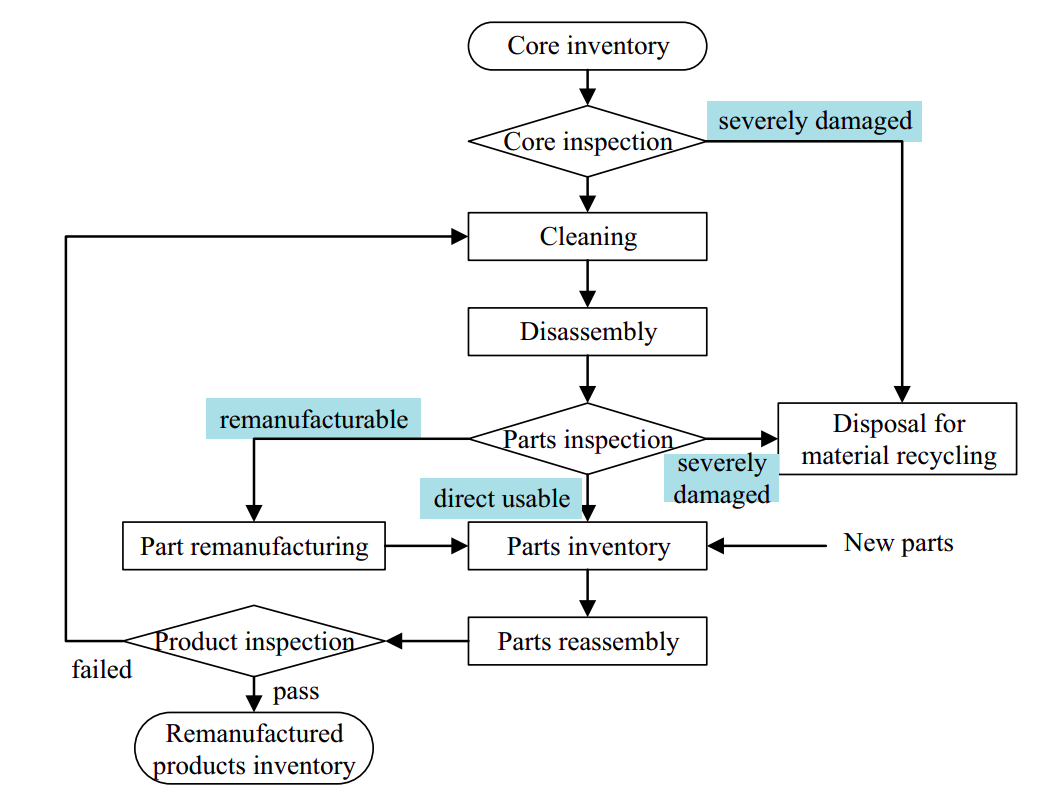
\includegraphics[width=\linewidth]{130quantification/internal/cei/zhao2021reman.png}
    \caption[An example of a generic remanufacturing process for vehicle components]{An example of a generic remanufacturing process for vehicle components~\cite{zhao2021reman}}
    \label{fig:remanufacturing}
\end{figure}
\FloatBarrier
\sectionEndlines
\clearpage


\subsubsection{Relevance of Remanufacturing and Refurbishing in FutuRaM's Waste Streams}

\wasteSubsubsecBATT
\begin{itemize}
    \item Electric Vehicle Batteries: Remanufacturing can involve replacing degraded cells or modules to extend their lifespan, thereby conserving lithium and cobalt.
    \item Laptop Batteries: Through remanufacturing, individual cells within the battery pack can be replaced or upgraded, enhancing the overall battery life and efficiency.
\end{itemize}

\wasteSubsubsecELV
\begin{itemize}
    \item Automotive Engines: Remanufacturing can include refurbishing engine components, such as pistons and bearings, to restore performance and efficiency.
    \item Transmission Systems: Rebuilding transmission systems with replaced or refurbished gears and bearings can significantly extend the life of the vehicle.
\end{itemize}

\wasteSubsubsecWEEE
\begin{itemize}
    \item Smartphones: Remanufacturing can involve replacing batteries, screens, and other components to restore them to like-new condition.
    \item Printers and Copiers: Components such as toner cartridges, drums, and fusers can be remanufactured to extend their service life and improve functionality.
\end{itemize}

\wasteSubsubsecCDW
\begin{itemize}
    \item Structural Steel Elements: In construction and demolition, steel beams and columns can be refurbished and reused in new construction projects.
    \item Wooden Beams and Flooring: Wooden elements can be remanufactured through processes like sanding, treating, and reinforcing for reuse in construction.
\end{itemize}


\sectionEndlines
\clearpage

\clearpage
\subsection{Remanufacturing: \textit{Scenarios}}

\boxws{This section will be filled out with the details of exactly how this parameter is incorporated into your stock and flow models}


\subsubsection{Global trends}


\subsubsection{Summary}

\boxreview{This summary will be compiled once the individual waste stream sections for each parameter are complete.}

\clearpage

\subsubsection[Scenario I: Business-as-usual]{\iconBAU Scenario I: Business-as-usual}

xx \\


\wasteSubsubsubsecBATT

\wasteSubsubsubsecCDW

\wasteSubsubsubsecELV

\wasteSubsubsubsecMIN

\wasteSubsubsubsecSLASH

\wasteSubsubsubsecWEEE

\subsectionEndline
\clearpage

\subsubsection[Scenario II: Recovery]{\iconREC Scenario II: Recovery}

xx \\


\wasteSubsubsubsecBATT

\wasteSubsubsubsecCDW

\wasteSubsubsubsecELV

\wasteSubsubsubsecMIN

\wasteSubsubsubsecSLASH

\wasteSubsubsubsecWEEE

\subsectionEndline
\clearpage


\subsubsection[Scenario III: Circularity]{\iconCIR Scenario III: Circularity}

xx \\


\wasteSubsubsubsecBATT

\wasteSubsubsubsecCDW

\wasteSubsubsubsecELV

\wasteSubsubsubsecMIN

\wasteSubsubsubsecSLASH

\wasteSubsubsubsecWEEE

\sectionEndlines
\clearpage
\clearpage

\subsection{The Sharing Economy: \textit{Description}}\cite{dabbous2021sharing, pwc2016sharing, dggrow2018sharing, dggrow2018sharingenv, dabbous2021sharing, ps2share2017sharing, zhu2021sharing}

\subsubsection{Definition}
The sharing economy is a socio-economic system that emphasizes the
collaborative sharing of goods and services via community-based online
platforms. It represents a shift from traditional ownership, where assets were
exclusively leased, to a flexible model allowing for both personal use and
lease. This flexibility is a hallmark of the sharing economy, which has grown
significantly in response to advancements in technology, such as e-commerce and
mobile connectivity, coupled with a societal push for more sustainable living
and efficient resource use.


\boxparameter{The sharing economy}{Stable}{Stable}{Strong increase}


\subsubsection{Context}
As the concept of ownership transforms, particularly among the younger
generation, the sharing economy has increasingly taken root in the EU market.
This shift towards more communal and cost-effective ways of accessing goods and
services is supported by a new wave of consumer behavior, underpinned by
technological innovation and a pressing need to reduce environmental waste and
resource duplication.

While the sharing economy is broad and its definition fluid, it is often
associated with collaborative consumption, though the two can differ in motives
and mechanisms. Collaborative consumption may span consumer-to-consumer and
business-to-consumer interactions, whereas the sharing economy typically
operates within the consumer-to-consumer sphere. The sharing economy is thereby
defined as an innovative marketplace where entities engage in the distribution
and utilization of products and resources, with scalability achieved through
technological means.

This socio-economic model has not only disrupted traditional business sectors
but has also brought new value to the global economy, with rapid and profound
market penetration. Financial forecasts have been bullish, with revenue for
sharing platform providers expected to increase from USD 18.6 billion in 2017
to an estimated USD 40.2 billion in 2022. Moreover, the overall value of the
global sharing economy is projected to expand significantly, from USD 14
billion in 2014 to USD 335 billion in 2025, reflecting an unprecedented growth
trajectory over a mere twelve years\cite{zhu2021sharing}. Such growth reflects
the substantial economic potential and transformative power of the sharing
economy in contemporary markets.

\subsubsection{Scope within the EU Economy}
The sharing economy has made a significant economic contribution to the EU,
with an estimated €26.5 billion added to the GDP in 2016~\cite{pwc2016sharing}.
This figure is expected to grow, indicating the sharing economy's increasing
importance within the EU's economic structure.

\subsubsection{Environmental Prospects}~\cite{dabbous2021sharing, pwc2016sharing, dggrow2018sharingenv}

See~\cite{zhu2021sharing} Table 2 for a summary of the studies on the
environmental impacts of the sharing economy.

The sharing economy has the potential to reshape consumption behaviors and
reduce environmental impacts by promoting the sustainable use of resources.
This economic paradigm encourages the efficient employment of underutilised
goods, which can lead to a decrease in the need for new products, thus
conserving resources and mitigating greenhouse gas emissions. It fosters a
lifestyle that lessens the adverse environmental effects of consumption while
improving quality of life.

Central to the sharing economy is the promotion of moderate consumption
patterns. This approach aims to reduce the excessive purchasing habits of
certain populations to alleviate ongoing environmental harm. The sharing
economy's alignment with green consumption practices encompasses waste
reduction, energy conservation, and the adoption of sustainable resources, all
while managing and moderating excessive consumption.

The impact on the fast fashion industry serves as a pertinent example, with the
sector's frequent turnover to keep pace with changing trends leading to
significant textile waste. Collaborative consumption through the sharing
economy can mitigate this waste by encouraging the reuse and extension of
clothing's service life. Clothing libraries are an example of how the sharing
economy can provide environmental benefits by prolonging the usable life of
garments.

Eco-efficiency is enhanced when environmental resources are utilised more
effectively, leading to an increased use of products with minimal environmental
burden. This is exemplified in collaborative fashion consumption, which could
reduce the prevalent overconsumption in the fashion industry. By facilitating
the exchange of underused clothing, the sharing economy can increase the
lifecycle of garments and encourage the production of more durable products.

Beyond the realm of fashion, car sharing and shared accommodation are other
aspects of the sharing economy with notable environmental benefits. Car sharing
can significantly reduce the number of vehicles needed, thereby lowering
exhaust emissions. Similarly, shared accommodations have been associated with
significantly lower carbon dioxide emissions compared to conventional hotel
stays.

However, the question of whether the sharing economy indeed delivers
environmental benefits remains contested.~\cite{zhu2021sharing,
  geissinger2019sharing} Detractors highlight the potential for an increase in
environmental burdens, particularly if the heightened usability of shared goods
escalates greenhouse gas emissions. The environmental and socio-economic
impacts engendered by the collaborative economy are intricate and highly
variable across different business models. Generally speaking, collaborative
consumption models that optimise the use of existing assets tend to exhibit a
lower environmental footprint compared to their traditional counterparts.
Nevertheless, there is a risk that the financial savings afforded by
collaborative consumption could spur additional spending and consumption, which
might negate the direct environmental savings. Despite such reservations, the
prevailing view is that the sharing economy, by transforming consumption from
ownership to communal use, can yield considerable environmental advantages.

\subsubsection{Implications for Waste Streams}

The adoption of sharing economy principles can influence various waste streams,
including:

\begin{itemize}
  \item \textbf{BATT (Waste Batteries):} As devices are shared and utilized more efficiently, the frequency of battery disposal could decline, mitigating the waste battery stream.
  \item \textbf{CDW (Construction and Demolition Waste):} The sharing of construction equipment and machinery could potentially slow down the turnover rate of these items, reducing associated waste.
  \item \textbf{WEEE (Waste Electrical and Electronic Equipment):} Sharing electronic devices extends their lifecycle and reduces the rate at which they are discarded, thereby impacting electronic waste volumes.
  \item \textbf{ELV (End-of-Life Vehicles):} A shift towards car-sharing services could reduce the demand for manufacturing new vehicles, potentially leading to a downturn in the generation of automotive waste.
\end{itemize}

The trajectory of the sharing economy indicates a shift towards collective
usage patterns. Its continuing evolution could play a critical role in the
future of critical raw material recovery systems by affecting demand and the
lifecycle of products, which, in turn, influences waste stream outputs. The
broader implications for the raw materials sector are significant, suggesting a
possible recalibration of recovery strategies for critical raw materials in
light of emerging consumption patterns.

\subsubsection{Challenges in Measuring Sharing Economy Growth}

Identifying a universal metric for the growth of the sharing economy is
challenging due to its diverse and dynamic nature. Current measures, such as
STOXX Global sharing economy indices, Solactive Sharing Economy Index and the
INDXX US Sharing Economy Index, largely revolve around the market sizes of
prominent sharing economy companies, such as Uber and Airbnb. These indices,
while useful, predominantly reflect the scalability of these businesses rather
than the sharing economy's broader impacts on production and waste reduction.

In the absence of a standardised metric, the assessment of the sharing
economy's expansion is often best approached through product-specific data.
This involves examining the adoption rates and usage trends of sharing services
at the product level to infer growth patterns. Such a detailed, product-centric
analysis allows for a closer inspection of the sharing economy's implications
on resource utilisation and waste generation, offering insights that aggregate
economic data may overlook.

\sectionEndlines
\clearpage
\clearpage
\subsection{The Sharing Economy: \textit{Scenarios}}

\boxws{This section will be filled out with the details of exactly how this parameter is incorporated into your stock and flow models}

\subsubsection{Summary}


\boxreview{This summary will be compiled once the individual waste stream sections for each parameter are complete.}

\clearpage

\subsubsection[Scenario I: Business-as-usual]{\iconBAU Scenario I: Business-as-usual}

xx \\


\wasteSubsubsubsecBATT

\wasteSubsubsubsecCDW

\wasteSubsubsubsecELV

\wasteSubsubsubsecMIN

\wasteSubsubsubsecSLASH

\wasteSubsubsubsecWEEE

\subsectionEndline
\clearpage

\subsubsection[Scenario II: Recovery]{\iconREC Scenario II: Recovery}

xx \\


\wasteSubsubsubsecBATT

\wasteSubsubsubsecCDW

\wasteSubsubsubsecELV

\wasteSubsubsubsecMIN

\wasteSubsubsubsecSLASH

\wasteSubsubsubsecWEEE

\subsectionEndline
\clearpage


\subsubsection[Scenario III: Circularity]{\iconCIR Scenario III: Circularity}

xx \\


\wasteSubsubsubsecBATT

\wasteSubsubsubsecCDW

\wasteSubsubsubsecELV

\wasteSubsubsubsecMIN

\wasteSubsubsubsecSLASH

\wasteSubsubsubsecWEEE

\sectionEndlines
\clearpage
\clearpage


\subsubsection{Conclusion}


\boxreview{This conclusion will be compiled once the individual waste stream sections for each parameter are complete.}


\sectionEndlines
\clearpage
\clearpage

\breaksection{Conclusion}

\boxreview{This conclusion will be compiled once the individual waste stream sections for each parameter are complete.}

% end of chapter
\chapterEndlines